%  ========================================================================
%  Copyright (c) 1985 The University of Washington
%
%  Licensed under the Apache License, Version 2.0 (the "License");
%  you may not use this file except in compliance with the License.
%  You may obtain a copy of the License at
%
%      http://www.apache.org/licenses/LICENSE-2.0
%
%  Unless required by applicable law or agreed to in writing, software
%  distributed under the License is distributed on an "AS IS" BASIS,
%  WITHOUT WARRANTIES OR CONDITIONS OF ANY KIND, either express or implied.
%  See the License for the specific language governing permissions and
%  limitations under the License.
%  ========================================================================
%

% Documentation for University of Washington thesis LaTeX document class
% by Jim Fox
% fox@washington.edu
%
%    Revised 2020/02/24, added \caption()[]{} option.  No ToC.
%
%    Revised for version 2015/03/03 of uwthesis.cls
%    Revised, 2016/11/22, for cleanup of sample copyright and title pages
%
%    This document is contained in a single file ONLY because
%    I wanted to be able to distribute it easily.  A real thesis ought
%    to be contained on many files (e.g., one for each chapter, at least).
%
%    To help you identify the files and sections in this large file
%    I use the string '==========' to identify new files.
%
%    To help you ignore the unusual things I do with this sample document
%    I try to use the notation
%       
%    % --- sample stuff only -----
%    special stuff for my document, but you don't need it in your thesis
%    % --- end-of-sample-stuff ---


%    Printed in twoside style now that that's allowed
%
 
\documentclass [11pt, proquest] {uwthesis}[2020/02/24]
 
%
% The following line would print the thesis in a postscript font 

% \usepackage{natbib}
% \def\bibpreamble{\protect\addcontentsline{toc}{chapter}{Bibliography}}

\setcounter{tocdepth}{1}  % Print the chapter and sections to the toc
 

% ==========   Local defs and mods
%

% --- sample stuff only -----
% These format the sample code in this document

\usepackage{alltt}  % 
\newenvironment{demo}
  {\begin{alltt}\leftskip3em
     \def\\{\ttfamily\char`\\}%
     \def\{{\ttfamily\char`\{}%
     \def\}{\ttfamily\char`\}}}
  {\end{alltt}}
 
% metafont font.  If logo not available, use the second form
%
% \font\mffont=logosl10 scaled\magstep1
\let\mffont=\sf
% --- end-of-sample-stuff ---
 

\usepackage{commands}

\begin{document}
 
% ==========   Preliminary pages
%
% ( revised 2012 for electronic submission )
%

\prelimpages
 
%
% ----- copyright and title pages
%
\Title{Projectivity of moduli spaces of complexes}
\Author{Tuomas Tajakka}
\Year{2021}
\Program{Mathematics}

\Chair{Jarod Alper}{Associate Professor}{Department of Mathematics}
\Signature{Max Lieblich}
\Signature{Bianca Viray}
%\Signature{etc}

\copyrightpage

\titlepage  

 
%
% ----- signature and quoteslip are gone
%

%
% ----- abstract
%


\setcounter{page}{-1}
\abstract{%
Determinantal line bundle techniques provide an alternative to using Geometric Invariant Theory in constructing moduli spaces as projective varieties -- Faltings, Kollar. Something about Bridgeland stability and no GIT. 
}
 
%
% ----- contents & etc.
%
\tableofcontents
%\listoffigures
%\listoftables  % I have no tables
 
%
% ----- glossary 
%
\iffalse
\chapter*{Glossary}      % starred form omits the `chapter x'
\addcontentsline{toc}{chapter}{Glossary}
\thispagestyle{plain}
%
\begin{glossary}
\item[argument] replacement text which customizes a \LaTeX\ macro for
each particular usage.
\item[back-up] a copy of a file to be used when catastrophe strikes
the original.  People who make no back-ups deserve
no sympathy.
\item[control sequence] the normal form of a command to \LaTeX.
\item[delimiter] something, often a character, that indicates
the beginning and ending of an argument.
More generally, a delimiter is a field separator.
\item[document class] a file of macros that tailors \LaTeX\ for
a particular document.  The macros described by this thesis
constitute a document class.
\item[document option] a macro or file of macros
that further modifies \LaTeX\ for
a particular document.  The option {\tt[chapternotes]}
constitutes a document option.
\item[figure] illustrated material, including graphs,
diagrams, drawings and photographs.
\item[font] a character set (the alphabet plus digits
and special symbols) of a particular size and style.  A couple of fonts
used in this thesis are twelve point roman and {\sl twelve point roman
slanted}.
\item[footnote] a note placed at the bottom of a page, end of a chapter,
or end of a thesis that comments on or cites a reference
for a designated part of the text.
\item[formatter] (as opposed to a word-processor) arranges printed
material according to instructions embedded in the text.
A word-processor, on the other hand, is normally controlled
by keyboard strokes that move text about on a display.
\item[\LaTeX] simply the ultimate in computerized typesetting.
\item[macro]  a complex control sequence composed of 
other control sequences.
\item[pica] an archaic unit of length.  One pica is twelve points and
six picas is about an inch.
\item[point] a unit of length.  72.27 points equals one inch.
\item[roman]  a conventional printing typestyle using serifs.
the decorations on the ends of letter strokes.
This thesis is set in roman type.
\item[rule] a straight printed line; e.g., \hrulefill.
\item[serif] the decoration at the ends of letter strokes.
\item[table] information placed in a columnar arrangement.
\item[thesis] either a master's thesis or a doctoral dissertation.
This document also refers to itself as a thesis, although it
really is not one.
 
\end{glossary}
\fi
%
% ----- acknowledgments
%
\acknowledgments{% \vskip2pc
  % {\narrower\noindent
  I want to thank mom, dad, friends, Jarod etc.
  % \par}
}

%
% ----- dedication
%
\dedication{\begin{center}In memoriam Dave DiMuro\end{center}}

%
% end of the preliminary pages
 
 
 
%
% ==========      Text pages
%

\textpages
 
% ========== Chapter 1
 
\chapter{Introduction}
May I introduce
\chapter{Background on sheaves and complexes and their moduli}\label{chapter:background}
In this chapter we collect and summarize several key notions and results needed in the main body of the work. We consider schemes over a fixed  algebraically closed field $k$.

\section{Local properties of sheaves}
Let $X$ be a regular, noetherian, integral scheme of dimension $n$. The dimension of a coherent sheaf $F$ on $X$ is the dimension of its support $\Supp(F)$. A $d$-dimensional sheaf $F$ is called \textbf{pure} if all its associated points have dimension $d$, or equivalently if $\Hom(G, F) = 0$ for all sheaves $G$ of dimension less than $d$. A coherent sheaf $F$ of dimension $d$ has a unique filtration
\[ F_0 \subs F_1 \subs \ldots \subs F_{d-1} \subs F_d = F \]
where $F_i$ is the union of all subsheaves of dimension at most $i$, so that $F_i/F_{i-1}$ is either zero or pure of dimension $i$ for each $i$. A \textbf{torsion-free} sheaf is a pure sheaf of dimension $n$. A torsion-free sheaf is locally free in codimension 1. The \textbf{rank} of $F$ is denote $\rk(F)$ and defined as the dimension of the stalk of $F$ at the generic point of $X$.

The \textbf{dual} of $F \in \Coh(X)$ is the sheaf $F^\vee = \sHom(F, \Oh_X)$. The canonical map $F \to F^\dd$ to the \textbf{double dual} of $F$ is injective whenever $F$ is torsion-free, and we say that $F$ is \textbf{reflexive} if this map is an isomorphism. A reflexive sheaf is locally free in codimension 2.

\tuomas{Lemmas about the behavior of reflexive sheaves here? Such as Ext groups with 0-dimensional sheaves etc. Where are they even needed?}

\section{Stability of sheaves}
Let $X$ be a smooth, projective variety of dimension $n$ with a very ample divisor $H \subs X$. We denote the Hilbert polynomial of a coherent sheaf $F$ by
\[ P(F, m) = \chi(X, F \otimes \Oh_X(mH)) = \sum_{i=0}^n (-1)^i \dim H^i(X, F \otimes \Oh_X(mH)), \]
and, if $\dim(F) = n$, define the \textbf{reduced Hilbert polynomial} of $F$ as
\[ p(F,m) = \frac{1}{\rk(F)} P(F, m). \]
A torsion-free sheaf $F$ is \textbf{Gieseker-stable} (resp. \textbf{Gieseker-semistable}) if for any proper, nonzero subsheaf $F' \subs F$ we have 
\[ p(F', m) < p(F, m) \qquad (\text{resp.} \quad p(F', m) \le p(F, m)), \]
where we compare polynomials by asymptotic inequality, or equivalently by lexicographically comparing their coefficients. Note that the first inequality holds automatically for subsheaves $F'$ with $\rk(F') = \rk(F)$, so we can assume $\rk(F') < \rk(F)$ in the definition.

By the Hirzebruch-Riemann-Roch formula, the coefficient of the degree $n-1$ term in $p(F, m)$ is the quantity
\[ \mu(F) = \frac{H^{n-1} \cdot c_1(F)}{\rk(F)}, \]
which we call the \textbf{$H$-slope}, or simply \textbf{slope}, of $F$. We say $F$ is \textbf{$\mu$-stable} (resp. \textbf{$\mu$-semistable}) if it is torsion-free and for any subsheaf $F' \subs F$ of smaller rank we have 
\[ \mu(F') < \mu(F) \qquad (\text{resp.} \quad \mu(F') \le \mu(F)). \]
We have the evident implications
\begin{center}
    $\mu$-stable $\implies$ Gieseker-stable $\implies$ Gieseker-semistable $\implies$ $\mu$-semistable.
\end{center}
Moreover, if $\gcd(\rk(F), H^{n-1}\cdot c_1(F)) = 1$, then all four notions are equivalent. To see this, let $F' \subs F$ be a subsheaf with $\mu(F') = \mu(F)$, or equivalently
\[ \rk(F) (H^{n-1} \cdot c_1(F')) = \rk(F') (H^{n-1}\cdot c_1(F)). \]
Since $\rk(F)$ divides the right hand side, it must divide $\rk(F')$, so that $\rk(F') = \rk(F)$. 

A torsion-free sheaf $F$ is called \textbf{$\mu$-polystable} if it is a direct sum $F = \oplus_i F_i$ of $\mu$-stable sheaves $F_i$ with $\mu(F_i) = \mu(F)$. Any $\mu$-semistable sheaf $F$ has a \textbf{Jordan-H\"older filtration}
\[ 0 = F_0 \subsetneq F_1 \subsetneq \ldots \subsetneq F_{m-1} \subsetneq F_m = F \]
where the successive quotients $\gr_i(F) \coloneqq F_i/F_{i-1}$ are $\mu$-stable with $\mu(\gr_i(F)) = \mu(E)$. The sheaf $\gr(F) \coloneqq \oplus_i \gr_i(F)$ is called the \textbf{associated graded} of $F$. The Jordan-H\"older filtration is not necessarily unique, but the associated graded is unique up to isomorphism. Two $\mu$-semistable sheaves $F_1$ and $F_2$ are called \textbf{S-equivalent} if $\gr(F_1) \cong \gr(F_2)$. Each equivalence class is represented by a unique polystable sheaf.

Any torsion-free sheaf $E$ admits a \textbf{Harder-Narasimhan filtration}
\[ 0 = E_0 \subsetneq E_1 \subsetneq \ldots \subsetneq E_{m-1} \subsetneq E_m = E \]
where the successive quotients $E_i/E_{i-1}$ are $\mu$-semistable with $\mu(E_1/E_0) > \mu(E_2/E_1) > \cdots > \mu(E_m/E_{m-1})$. The Harder-Narasimhan filtration is uniquely determined by $E$.

We define polystability, Jordan-H\"older filtrations, the associated graded, S-equivalence, and Harder-Narasimhan filtrations analogously for Gieseker-stability. It will be clear from context which type of stability we mean.

We recall the following. If $E$ and $F$ are either (a) Gieseker-stable sheaves with the same reduced Hilbert polynomial, or (b) $\mu$-stable reflexive sheaves with the same slope, then either $E \cong F$ or $\Hom(E, F) = 0$. As a consequence, if $E \cong \oplus_{i=1}^m E_i^{\oplus r_i}$ is either a Gieseker-polystable sheaf or $\mu$-polystable reflexive sheaf, with $E_i$ and $E_j$ nonisomorphic when $i \neq j$, then
\[ \Aut(E) \cong \GL_{r_1} \times \cdots \times \GL_{r_m} \]

As will be discussed below, moduli spaces of Gieseker-semistable sheaves can be constructed as projective schemes using GIT. While $\mu$-stability lacks this benefit, its utility comes from various permanence properties it enjoys. The most relevant for us is that $\mu$-stability is preserved under restriction to a general divisor. The following result is attributed to Mehta and Ramanathan.

\begin{thm}[\hspace{-0.3em} {\cite[Theorem 7.2.1, Theorem 7.2.8]{HL}}]\label{mehta-ramanathan}
    Let $X$ be a smooth, projective variety over an algebraically closed field with a very ample divisor $H$. Let $F$ be a $\mu$-semistable (resp. $\mu$-stable) sheaf on $X$. There exists an integer $a_0$ such that for $a \ge a_0$ and a general smooth divisor $D \in |a H|$, the restriction $F|_D$ is $\mu$-semistable (resp. $\mu$-stable).
\end{thm}

The integer $a_0$ in the theorem depends on the sheaf $F$. In characteristic 0, we get the following stronger result for restricting $\mu$-semistable sheaves to complete intersections of divisors, attributed to Flenner.

\begin{thm}[\hspace{-0.3em} {\cite[Theorem 7.1.1, Theorem 7.2.8]{HL}}]\label{flenner}
    Let $X$ be a smooth, projective variety of dimension $n \ge 2$ over an algebraically closed field of characteristic 0, and let $H \subs X$ be a very ample divisor. Let $r$ and $l$ be integers with $r > 0$ and $1 \le l \le n-1$. There exists an integer $a_0$, depending on $r$ and $l$, such that if $a \ge a_0$ and $F$ is a $\mu$-semistable sheaf on $X$, the restriction $F|_{D_1 \cap \cdots \cap D_l}$ to a complete intersection of general divisor $D_1, \ldots, D_l \in |a H|$ is again $\mu$-semistable.
\end{thm}


\section{Derived categories}
We now recall some basic notions of derived categories. Let $X$ be a scheme of finite type over $k$. If
\[ E: \quad \cdots \to E_{i-1} \xrightarrow{d_{i-1}} E_i \xrightarrow{d_i} E_{i+1} \to \cdots \]
is a complex of coherent sheaves on $X$, we denote by $\sH^i(E) = \ker d_i/\img d_{i-1}$ its $i$th cohomology sheaf. A map $E \to F$ of complexes is a \textbf{quasi-isomorphism} if it induces an isomorphism $\sH^i(E) \xrightarrow{\sim} \sH^i(F)$ for all $i$. We denote by $D^b(X)$ the derived category of $X$, which is a triangulated category whose objects are bounded complexes of coherent sheaves and whose morphisms are maps of chain complexes and formal inverses of quasi-isomorphisms. An exact triangle
\[ E \to F \to G \]
in $D^b(X)$ induces an exact sequence
\[ \cdots \to \sH^i(E) \to \sH^i(F) \to \sH^i(G) \to \sH^{i+1}(E) \to \cdots \]
in $\Coh(X)$. Any morphism $\phi: E \to F$ in $D^b(X)$ can be completed to an exact triangle
\[ E \xrightarrow{\phi} F \to \cone(\phi). \]

The category of coherent sheaves $\Coh(X)$ embeds as a full subcategory of $D^b(X)$ as complexes $E$ with $\sH^i(E) = 0$ for $i \neq 0$. For $E, F \in \Coh(X)$ we have identifications
\[ \Ext^i(E,F) = \Hom_{D^b(X)}(E, F[i]) = \Hom_{D^b(X)}(E[-i], F) \quad \text{for all\;} i. \]
We often use this notation even when $E$ and $F$ are not sheaves. Moreover, if $X$ is smooth and projective of pure dimension $n$, the canonical sheaf $\om_X$ induces a duality
\[ \Hom_{D^b(X)}(E, F) \cong \Hom_{D^b(X)}(F, E \otimes \om_X[n])^\vee, \]
functorial in $E, F \in D^b(X)$, extending the usual Serre duality.

A proper morphism $X \to Y$ of smooth varieties over $k$ induces an adjoint pair of exact functors
\[ L f^*: D^b(Y) \to D^b(X), \qquad R f_*: D^b(X) \to D^b(Y). \]
extending the pullback and pushforward along $f$. When $f$ is a closed embedding, we call $L f^*$ the derived restriction and denote $L f^*E = E|^\LL_X$. If on the other hand $f$ is the structure map $X \to \Spec k$, we denote $R f_* = R\Ga(X, -)$ and call the cohomology sheaves of $R\Ga(X, E)$ the hypercohomology groups of $E$ and denote them by $\Hh^i(X, E)$.

An object $E \in D^b(X)$ induces a derived tensor product $(-) \otimes^\LL E: D^b(X) \to D^b(X)$, derived local homs 
\[ R\sHom_X(E,-): D^b(X) \to D^b(X) \quad \text{and} \quad R\sHom(-, E): D^b(X)^{\text{op}} \to D^b(X), \]
as well as global homs 
\[ R\Hom_X(E,-): D^b(X) \to D^b(\Spec k) \quad  \text{and} \quad R\Hom(-, E): D^b(X)^{\text{op}} \to D^b(\Spec k), \]
each functorial in $E$.

\subsection{Hearts and tilting}
The subcategory $\Coh(X) \subs D^b(X)$ has the special feature that any object $E \in D^b(X)$ has a unique filtration
\[ 0 = E_0 \to E_1 \to \cdots \to E_{m-1} \to E_m = E \]
such that $\cone(E_{i-1} \to E_i)$ lies in $\Coh(X)[k_i]$ for some $k_i$, and $k_1 > k_2 > \cdots > k_m$ -- this is just the usual filtration of $E$ by its cohomology sheaves $\sH^i(E)$. Abstracting this property gives rise to the following definition.
\begin{defn}
    A {\bf heart of a bounded t-structure} is a full additive subcategory $\sA \subs D^b(X)$ such that
    \begin{enumerate}[(i)]
        \item $\Hom(A, B[i]) = 0$ for any $A, B \in \sA$ and $i < 0$,
        \item For any $E \in D^b(X)$, there exists a filtration
        \begin{center}
        \begin{tikzpicture}
        \matrix (m) [matrix of math nodes, row sep=3em, column sep=3em]
        { 0 = E_0 & E_1 & \cdots & E_{m-1} & E_m = E \\
        & A_1[k_1] & \cdots & A_{m-1}[k_{m-1}] & A_m[k_m] \\};
        \path[->] 
        (m-1-1) edge node[auto] {$ $} (m-1-2)
        (m-1-2) edge node[auto] {$ $} (m-1-3)
        (m-1-3) edge node[auto] {$ $} (m-1-4)
        (m-1-4) edge node[auto] {$ $} (m-1-5)
        (m-1-2) edge node[auto] {$ $} (m-2-2)
        (m-1-4) edge node[auto] {$ $} (m-2-4)
        (m-1-5) edge node[auto] {$ $} (m-2-5)
        ;
        \path[dashed,->]
        (m-2-5) edge node[auto,swap] {$ [1] $} (m-1-4)
        (m-2-2) edge node[auto,swap] {$ [1] $} (m-1-1)
        (m-2-4) edge node[auto,swap] {$ [1] $} (m-1-3)
        ;        
        \end{tikzpicture}
        \end{center}
        with $A_1, \ldots, A_m \in \sA$, and $k_1 > k_2 > \cdots > k_m$.
    \end{enumerate}
\end{defn}
It follows from (i) that the filtration in (ii) is unique. Moreover, a heart $\sA$ turns out to be abelian, a short exact sequence in $\sA$ begin simply an exact triangle in $D^b(X)$ whose three vertices lie in $\sA$.

A method for producing new hearts from old is provided by tilting with respect to a torsion pair.
\begin{defn}
    A {\bf torsion pair} on an abelian category $\sA$ is a pair $(\sT, \sF)$ of full additive subcategories of $\sA$, such that
    \begin{enumerate}[(i)]
        \item $\Hom(T, F) = 0$ for any $T \in \sT,$ and $F \in \sF$,
        \item for any $E \in \sA$, the exists a short exact sequence $0 \to T \to E \to F \to 0$ with $T \in \sT$ and $F \in \sF$.
    \end{enumerate}
\end{defn}
It follows again from (i) that the short exact sequence in (ii) is unique. The basic example of a torsion pair is $(\sT, \sF) \subs \Coh(X)$ where $\sT$ and $\sF$ are the full subcategory of torsion sheaves and torsion-free sheaves respectively.
\begin{defn}
    Given a torsion pair $(\sT, \sF)$ on a heart of a bounded t-structure $\sA \subs D^b(X)$, the {\bf tilt} of $\sA$ with respect $(\sT, \sF)$ is the full subcategory
    \[ \sA^\# = \langle \sF, \sT[-1] \rangle \]
    of $D^b(X)$ consisting of objects that fit in an exact triangle
    \[ F \to E \to T[-1] \]
    with $F \in \sF$ and $T \in \sT$.
\end{defn}
The tilt of a heart is again a heart, and in particular abelian.

\section{Good moduli spaces}
A good moduli space is a generalization to algebraic stacks of the usual coarse moduli space associated to a Deligne-Mumford stack or a gerbe. In a sense, a good moduli space is an algebraic space that most closely approximates the stack. Based on ideas from Geometric Invariant Theory, Alper gave the definition and developed the basic theory of good moduli spaces in \cite{AlperGMS}.

Let $\sM$ be an algebraic stack. A quasi-compact, quasi-separated morphism $\pi: \sM \to M$ to an algebraic space $M$ is called a {\bf good moduli space}, if 
\begin{itemize}
    \item the pushforward $\pi_*: \Qcoh(\sM) \to \Qcoh(M)$ is exact, and
    \item the natural map $\Oh_M \to \pi_*\Oh_\sM$ is an isomorphism.
\end{itemize}
We list a few basic properties of good moduli spaces.
\begin{prop}
    If $\pi: \sM \to M$ is a good moduli space, then the following hold. \begin{enumerate}[(i)]
        \item $\pi$ is surjective, universally closed, and induces a bijection on closed points.
        \item $\pi$ is universal for maps to algebraic spaces.
        \item For every geometric point $x: \Spec K \to \sM$ with closed image, the stabilizer group $G_x$ is linearly reductive.
        \item If $\sM$ is of finite type over a field, then so is $M$, and $\pi_*$ preserves coherence.
    \end{enumerate}
\end{prop}

We recall the following criterion \cite[Theorem 10.3]{AlperGMS} for a locally free sheaf on $\sM$ to descend to the good moduli space $M$. 
\begin{prop}\label{vbtogms}
    If $\pi: \sM \to M$ is a good moduli space and $\sM$ is locally noetherian, then the pullback morphism $\pi^*: \Coh(M) \to \Coh(\sM)$ induces an equivalence of categories between locally free sheaves on $M$ and those locally free sheaves $\sF$ on $\sM$ such that for every geometric point $x: \Spec k \to \sM$ with closed image, the induced representation $x^*\sF$ of the stabilizer $G_x$ is trivial.
\end{prop}

The existence of a good moduli space for a given algebraic stack is a subtle question. One answer is given in \cite{AHLH}, where for a large class of stacks the authors give necessary and sufficient conditions for existence of a good moduli space in terms of certain valuative criteria.

An important source of good moduli spaces is Geometric Invariant Theory. Let $X$ be a projective scheme, $G$ a linearly reductive algebraic group acting on $X$, and $L$ a $G$-linearized ample line bundle on $X$. Let $\sX = [X/G]$ denote the quotient stack. The invariant open subset $X^{\text{ss}}$ of semistable points with respect to $L$ gives an open substack $\sX^{\text{ss}}$, and the good GIT quotient $X^{\text{ss}}\sslash G$ is a good moduli space for $\sX^{\text{ss}}$. The closed points of $X^{\text{ss}}\sslash G$ are in bijection with the closed orbits of $X^{\text{ss}}$.

We will need the following in Chapters \ref{chapter:uhlenbeck} and \ref{chapter:pt}.
\begin{lem}\label{finitecurveextension}
    Let $\sM$ be an algebraic stack of finite type that admits a good moduli space $\pi: \sM \to M$ with $M$ proper. Let $C$ be a smooth, proper curve, and let $g: C \to M$ be a morphism. There exists a commutative diagram
    \begin{center}
    \begin{tikzpicture}
    \matrix (m) [matrix of math nodes, row sep=2em, column sep=2em]
    { C' & \sM  \\
    C & M \\};
    \path[->] 
    (m-1-1) edge node[auto] {$ f $} (m-1-2)
    (m-1-1) edge node[auto,swap] {$ \phi $} (m-2-1)
    (m-1-2) edge node[auto] {$ \pi $} (m-2-2)
    (m-2-1) edge node[auto,swap] {$ g $} (m-2-2)
    ;        
    \end{tikzpicture}
    \end{center}
    where $C'$ is smooth and proper and $\phi$ is finite.
\end{lem}
\begin{proof}
    Let $U \to \sM$ be a smooth surjection with $U$ a scheme of finite type. The fiber product $C \times_M U$ is also a scheme of finite type and $\pi_C: C \times_M U \to C$ is surjective. The scheme-theoretic fiber $\pi_C^{-1}(\eta)$ over the generic point $\eta \in C$ is of finite type over the function field of $C$, hence contains a closed point $\tau \in \pi_C^{-1}(\eta)$ whose residue field $K = \ka(\tau)$ is a finite extension of the function field $K(C) = \ka(\eta)$. Let $C_\tau$ denote the normalization of $C$ in the field $\ka(\tau)$. Since $U$ is of finite type, we can extend the map $\Spec K \to U$ over an open subscheme $V \subs C_\tau$ and obtain a commutative diagram
    \begin{center}
    \begin{tikzpicture}
    \matrix (m) [matrix of math nodes, row sep=2em, column sep=2em]
    { \Spec K & V & U & \sM \\
    & C_\tau & C & M \\};
    \path[right hook->] 
    (m-1-1) edge node[auto] {$ $} (m-1-2)
    (m-1-2) edge node[auto] {$ $} (m-2-2)
    ;
    \path[->]
    (m-1-2) edge node[auto] {$ $} (m-1-3)
    (m-1-3) edge node[auto] {$ $} (m-1-4)
    (m-1-4) edge node[auto] {$ \pi $} (m-2-4)
    (m-2-2) edge node[auto,swap] {$ $} (m-2-3)
    (m-2-3) edge node[auto] {$ g $} (m-2-4)
    ;        
    \end{tikzpicture}
    \end{center}
    By applying \cite[Theorem A.8]{AHLH} to the local rings of the finitely many points in the complement $C_\tau \setminus V$, we find a finite extension $K'$ of $K$ such that the normalization $C'$ of $C_\tau$ in $K'$ admits a map $C' \to \sM$.
\end{proof}

\section{Moduli stacks of sheaves and complexes}
Let $X$ be a smooth, projective variety over $k$. If $S$ is a $k$-scheme, a complex $E$ of quasi-coherent sheaves on $S \times X$ is called \textbf{perfect relative to $S$} or \textbf{$S$-perfect} if \'etale-locally on $S \times X$, it is quasi-isomorphic to a bounded complex of coherent sheaves flat over $S$. A complex on $X$ is \textbf{perfect} if it is perfect relative to the identity morphism, or in other words locally quasi-isomorphic to a bounded complex of locally free sheaf of finite rank. The \textbf{rank} of a perfect complex $E$ is the alternating sum of the ranks of the terms in a complex of locally free sheaves representing $E$.

An $S$-perfect complex is called \textbf{universally gluable} if for every geometric point $\Spec K \to S$, the complex $E_K = E|^\LL_{X_K} \in D^b(X_K)$ satisfies
\[ \Ext^i(E_K, E_K) = 0 \quad \text{for} \; i < 0. \]
We let $\sMom_X$ denote the stack on the big \'etale site of $k$-schemes that to a scheme $S$ associates the groupoid of universally gluable complexes on $S \times X$. On $\sMom_X \times X$ there is a universal $\sMom_X$-perfect complex.
\begin{thm}[\hspace{-0.3em} {\cite[Theorem 4.2.1]{lie06}}]\label{motherofallmoduli}
    The stack $\sMom_X$ is an algebraic stack locally of finite type over $k$.
\end{thm}
The stack $\sMom_X$ contains many useful open substacks.
For example, if $S$ is a scheme of finite type over $k$ and $E$ is an $S$-perfect complex on $S \times X$ such that for every $k$-point $s \in S$, the restriction $E_s \in D^b(X)$ lies in the heart of a bounded t-structure, then $E$ is universally gluable. In particular, any flat family of sheaves on $X$ is universally gluable. As another example, we say that a complex $E \in D^b(X)$ is \textbf{simple} if $\Hom(E,E) = k$ and $\Ext^i(E,E) = 0$ for $i < 0$. The substack $\sS pl \subs \sMom$ of simple complexes is a $\G_m$-gerbe over an algebraic space locally of finite presentation over $k$, see \cite{inaba}, \cite[Corollary 4.3.3]{lie06}.

\subsection{Moduli stacks of semistable sheaves}
Let $X$ be a smooth, projective variety of dimension $n$ over $k$ with a very ample divisor $H$. We let $K(X)$ denote the Grothendieck group of coherent sheaves on $X$. It has the structure of a filtered ring, where the product is induced by tensor product on locally free sheaves and the filtration is given by the codimension of the support of a coherent sheaf. We denote by $\Kn(X)$ the quotient of the Grothendieck group of coherent sheaves $K(X)$ by the kernel of the Euler pairing
\[ \chi: K(X) \times K(X) \to \Z, \quad \chi(E, F) = \sum_{i=0}^n (-1)^i \dim \Ext^i(E, F). \]
The group $\Kn(X)$ is a finitely generated free abelian group. For a class $v \in \Kn(X)$ with $\rk(v) > 0$, we obtain a sequence of open substacks
\[ \sM^{\mu-\text{s}}_X(v) \;\subs\; \sM^{\text{G-s}}_X(v) \;\subs\; \sM^{\text{G}}_X(v) \;\subs\; \sM^{\mu}_X(v) \qquad \subs \qquad \sMom \]
parameterizing, from left to right, $\mu$-stable, Gieseker-stable, Gieseker-semistable, and $\mu$-se\-mi\-stable torsion-free sheaves of class $v$. All four stacks are quasicompact and the first two are substacks of the stack $\sS pl$ of simple complexes and hence $\G_m$-gerbes over an algebraic space. If $\rk(v)$ and $H^{n-1}\cdot c_1(v)$ are coprime, then all four substacks coincide. In the stacks $\sM^{\text{G}}_X(v)$ and $\sM^{\mu}_X(v)$, two $k$-valued points representing S-equivalent sheaves have intersecting closures, which implies that a moduli variety of semistable sheaves can parameterize sheaves only up to S-equivalence.


\subsection{Projective moduli spaces of semistable sheaves}
A good moduli space for the stack $\sM^{\text{G}}_X(v)$ of Gieseker-semistable sheaves is obtained as a GIT quotient as follows. Since the family of semistable sheaves of class $v$ is bounded, there exist integers $n, m$ such for every semistable sheaf $F$, there exists a surjection $E \coloneqq \Oh_X(-m)^{\oplus n} \twoheadrightarrow F$ that induces an isomorphism on global sections $k^{\oplus n} = H^0(X, \Oh_X^{\oplus n}) \to H^0(X, F(m))$. Thus, if $P$ denotes the Hilbert polynomial of the class $v$, the semistable sheaves of class $v$ are represented by the points of an open subset $U$ of the Quot scheme $Q = \Quot(\Oh_X(-m)^{\oplus n}, P)$, giving rise to a surjective morphism
\[ \phi: U \to \sM^{\text{G}}_X(v). \]
The group $G = \SL(n)$ acts on the closure $\overline{U}$ by precomposing a quotient $E \twoheadrightarrow F$ with an automorphism of $E$, and the map $\phi$ is invariant under this action. Moreover, there is a natural linearized ample line bundle $L$ on $\overline{U}$ such that the semistable locus $\overline{U}^{\text{ss}}$ is precisely $U$, and we obtain a projective good moduli space 
\[ \sM^{\text{G}}_X(v) \to M^{\text{G}}_X(v) = U\sslash G \]
as the good GIT quotient. The closed points of $M^{\text{G}}_X(v)$ are in bijection with S-equivalence classes of Gieseker-semistable sheaves, and the open substack $\sM^{\text{G-s}}_X(v) \subs \sM^{\text{G}}_X(v)$ of stable sheaves induces an open subscheme $M^{\text{G-s}}_X(v) \subs M^{\text{G}}_X(v)$ parameterizing isomorphism classes of stable sheaves.

The situation is not as favorable with $\mu$-stability. In fact, the stack $\sM^{\mu}_X(v)$ of $\mu$-semistable sheaves does not have a good moduli space in general. For example if $I_p$ is the ideal sheaf of a closed point $p \in X$, then the sheaf $I_p \oplus \Oh_X$ is $\mu$-semistable, but its automorphism group is not linearly reductive. However, when $X$ is a surface, Jun Li \cite{li} constructed a projective scheme $M^{\text{Uhl}}_X(v)$, called the \textbf{Uhlenbeck compactification}, and a map $\pi: \sM^\mu_X(v) \to M^{\text{Uhl}}_X(v)$ giving rise to commutative diagram
\begin{center}
    \begin{tikzpicture}
    \matrix (m) [matrix of math nodes, row sep=4em, column sep=4em]
    { \sM^{\mathrm{G}}(v) & \sM^{\mu}(v) \\
    M^{\mathrm{G}}(v) & M^{\mathrm{Uhl}}(v) \\};
    \path[right hook->] 
    (m-1-1) edge node[auto] {$ _\mathrm{open\, emb.} $} (m-1-2)
    ;
    \path[->]
    (m-1-1) edge node[auto] {$ _\mathrm{gms} $} (m-2-1)
    (m-1-2) edge node[auto] {$ \pi $} (m-2-2)
    (m-2-1) edge node[auto] {$  $} (m-2-2)
    ;
    \end{tikzpicture}
\end{center}
To explain the set-theoretic behavior of $\pi$, recall that if $F$ is a $\mu$-semistable sheaf, the associated graded sheaf $\gr(F)$ is the direct sum of its Jordan-H\"older factors. Since $X$ is a surface, the double dual $\gr(F)^\dd$ is locally free and the quotient $\gr(F)^\dd/\gr(F)$ is supported at finitely many closed points of $X$. Two $\mu$-semistable sheaves $F_1$ and $F_2$ are identified by $\pi$ if and only if $\gr(F_1)^\dd$ and $\gr(F_2)^\dd$ are isomorphic and the quotients $\gr(F_1)^\dd/\gr(F_1)$ and $\gr(F_2)^\dd/\gr(F_2)$ are supported at the same points with the same lengths.

The goal of Chapter \ref{chapter:uhlenbeck} is to find a certain stack open substack $\sM^\si_X(v) \subs \sMom$ containing $\sM^\mu_X(v)$ whose good moduli space $M^\si_X(v)$ is identified with $M^{\text{Uhl}}_X(v)$. Unfortunately we only obtain a bijective morphism $M^{\text{Uhl}}_X(v) \to M^\si_X(v)$, and it remains open whether this map is an isomorphism.

In Chapter \ref{chapter:pt} we study a certain stack $\sM^{\text{PT}}_X(v)$ of complexes on a 3-fold $X$. We construct a morphism $\sM^{\text{PT}}_X(v) \to \overline{M}$ to a projective scheme $\overline{M}$ and show that the set-theoretic behavior of this map is closely analogous to that of the map to the Uhlenbeck compactification. In both chapters we heavily employ the technology of determinantal line bundles, which we now turn to.


\section{Determinantal line bundles}\label{section:determinantal}
Material for this section follows \cite[\href{https://stacks.math.columbia.edu/tag/0FJI}{Tag 0FJI}]{stacks-project}, \cite[\href{https://stacks.math.columbia.edu/tag/0FJW}{Tag 0FJW}]{stacks-project}, and \cite[Section 8.1]{HL}. The original exposition is \cite{KM76}.

Let $S$ be a scheme. The rule that sends a locally free sheaf $F$ to its determinant line bundle $\det(F) = \bigwedge^{\rk(F)} F$ extends to a functor
\[ \det: \{\mathrm{perfect\, complexes\, on\,} S\} \to \{\mathrm{invertible\,} \mathrm{sheaves\, on}\, S \}. \]
Moreover, for any short exact sequence
\[ 0 \to F' \to F \to F'' \to 0 \]
of locally free sheaves, there is a canonical isomorphism $\det(F) \to \det(F') \otimes \det(F'')$, so in particular we obtain an induced homomorphism of abelian groups
\[ \det: K_0(S) \to \Pic(S), \]
where $K_0(S)$ denotes the Grothendieck group of locally free sheaves on $S$. These constructions commute with pullbacks in the sense that if $\pi: S' \to S$ is a morphism of schemes and $F$ is a locally free sheaf or a perfect complex on $S$, then canonically $\det(\pi^* F) \cong \pi^*\det(F)$.

Let now $X$ be a smooth, projective variety over $k$, $S$ a scheme of finite type over $k$, and $\sE \in D^b(S \times X)$ an $S$-perfect complex. Note that since $X$ is smooth, we have $K_0(X) \cong K(X)$. Consider the diagram:
\begin{center}
    \begin{tikzpicture}
    \matrix (m) [matrix of math nodes, row sep=1em, column sep=1em]
    { & S \times X & \\
    S & & X \\};
    \path[->] 
    (m-1-2) edge node[auto,swap] {$ p $} (m-2-1)
    (m-1-2) edge node[auto] {$ q $} (m-2-3)
    ;
    \end{tikzpicture}
\end{center}
Any coherent sheaf $F$ on $X$ is perfect as an object of $D^b(X)$, and so the complex $\sE \otimes q^*F$ on $S \times X$ is again $S$-perfect. Thus, by \cite[\href{https://stacks.math.columbia.edu/tag/0B91}{Tag 0B91}]{stacks-project}, the derived pushforward $R p_* (\sE \otimes q^* F)$ is perfect on $S$. Composing with the determinant map gives a homomorphism of abelian groups
\[ \la_\sE: K(X) \to \Pic(S), \quad [F] \mapsto \det R p_*(\sE \otimes q^* F) \]
called the {\bf Donaldson morphism}. Moreover, since the formation of the pushforward $R p_*(\sE \otimes q^* F)$ commutes with base change, so does the formation of $\la_\sE$ in the sense that if $\pi: S' \to S$ is a morphism of schemes, then the composition
\[ K(X) \xrightarrow{\la_\sE} \Pic(S) \xrightarrow{\pi^*} \Pic(S') \]
equals $\la_{(\pi \times \id_X)^* \sE}$. In particular, the fiber of $\la_\sE(F)$ at a $k$-point $t \in S$ is identified with the 1-dimensional vector space
\[ \det R \Ga(X, \sE_t \otimes^\LL F) = \bigotimes_{i \in \Z} (\det \Hh^i(X, \sE_t \otimes^\LL F))^{(-1)^i}, \]
where $\sE_t$ denotes the restriction $\sE|^\LL_{\{t\} \times X} \in D^b(X)$.

We collect some of the basic properties of the Donaldson morphism in the following.
\begin{lem}\label{Donaldsonproperties}
    Let $w \in K(X)$.
    \begin{enumerate}[(i)]
        \item If $\sE \to \sF \to \sG$ is an exact triangle of $S$-perfect complexes on $S \times X$, then
        \[ \la_\sF(w) \cong \la_\sE(w) \otimes \la_\sG(w). \]
        
        \item If $F$ is a perfect complex on $X$, then
        \[ \la_{q^*F}(w) \cong \Oh_S. \]
        
        \item If $\sE$ is an $S$-perfect family of complexes of class $c \in K(X)$ on $S \times X$ and $G$ is a perfect complex on $S$, then
        \[ \la_{p^*G \otimes \sE}(w) = \la_\sE(w)^{\rk G} \otimes \det(G)^{\otimes \chi(c\cdot w)}. \]
    \end{enumerate}
\end{lem}

The Donaldson morphism respects numerical equivalence and hence a induces homomorphism
\[ \la_\sE: \Kn(X) \to \Num(S), \]
where $\Num(S)$ denotes $\Pic(S)$ modulo numerical equivalence, and furthermore extends to a linear map
\[ \la_\sE: \Kn(X)_\R \to \Num(S)_\R \]
of real vector spaces, where $\Kn(X)_\R = \Kn(X) \otimes \R$, and $\Num(S)_\R = \Num(S) \otimes \R$ is the group of real divisor classes.

This construction readily generalizes to algebraic stacks, and in particular, the Donaldson morphism lets us construct line bundles on the stack $\sMom_X$ and its open substacks. Let $\sM \subs \sMom_X$ be an open substack and $\sE$ the universal $\sM$-perfect complex on $\sM \times X$, and consider the diagram:
\begin{center}
    \begin{tikzpicture}
    \matrix (m) [matrix of math nodes, row sep=1em, column sep=1em]
    { & \sM \times X & \\
    \sM & & X \\};
    \path[->] 
    (m-1-2) edge node[auto,swap] {$ p $} (m-2-1)
    (m-1-2) edge node[auto] {$ q $} (m-2-3)
    ;
    \end{tikzpicture}
\end{center}
If $F$ is a coherent sheaf on $X$, we obtain the line bundle
\[ \la_\sE(F) \coloneqq \det(R p_*(\sE \otimes q^*F)) \]
on $\sM$, and this induces a group homomorphism
\[ \la_\sE: K(X) \to \Pic(\sM). \]


\subsection{Sections of determinantal line bundles}
In special situations the above construction of a determinantal line bundle also yields a canonical section of the dual of the line bundle. Namely, if $E \in D^b(S)$ is a perfect complex of rank 0 whose cohomology sheaves $\sH^i(E)$ vanish whenever $i \neq 0, 1$, then locally on $S$ the complex $E$ can be represented by a two-term complex of locally free sheaves
\[ \cdots \to 0 \to E_0 \xrightarrow{f} E_1 \to 0 \to \cdots, \quad \rk(E_0) = \rk(E_1). \]
The map $f$ induces a section $\det(f): \Oh_S \to \det(E_0)^\vee \otimes \det(E_1)$, and these local sections glue to a global section $\de_E \in \Ga(S, \det(E)^\vee)$. Moreover, the formation of this section commutes with pullbacks in the sense that if $\pi: S' \to S$ is a morphism of schemes, then the sections $\de_{\pi^*E}$ and $\pi^*\de_E$ are identified under the canonical isomorphism $\det(\pi^* E)^\vee \cong \pi^*(\det(E)^\vee)$. See \cite[\href{https://stacks.math.columbia.edu/tag/0FJX}{Tag 0FJX}]{stacks-project}. The following lemma gives a useful criterion for the existence and non-vanishing of a section.
\begin{lem}\label{detsection}
    Let $X$ be a smooth, projective variety and $S$ a scheme or an algebraic stack of finite type over $k$. Let $\sE \in D^b(S \times X)$ be an $S$-perfect complex, and let $F$ be a coherent sheaf on $X$.
    \begin{enumerate}[(a)]
        \item If for all $k$-points $t \in S$, we have $\Hh^i(X, \sE_t \otimes F) = 0$ whenever $i \neq 0, 1$, and 
        \[ \chi(X, \sE_t \otimes^\LL F) = \dim \Hh^0(X, \sE_t \otimes^\LL F) - \dim \Hh^1(X, \sE_t \otimes^\LL F) = 0, \]
        then the line bundle $\la_\sE(F)^\vee$ on $S$ has a canonical section $\de_F$.
        \item In addition, if for some $t \in S$ we have 
        \[ \Hh^0(X, \sE_t \otimes^\LL F) = \Hh^1(X, \sE_t \otimes^\LL F) = 0, \]
        then the section $\de_F$ is nonzero at $t$.
    \end{enumerate}
\end{lem}
\begin{proof}
    For (a), cohomology and base change implies that $R^i p_*(\sE \otimes q^* F) = 0$ for $i \neq 0,1$, and thus locally on $S$, the object $R p_*(\sE \otimes q^*F)$ can be represented by a complex
    \[ \cdots \to 0 \to \sG_0 \xrightarrow{f} \sG_1 \to 0 \to \cdots \]
    where $\sG_0$ and $\sG_1$ are locally free of finite rank. By \cite[\href{https://stacks.math.columbia.edu/tag/0B91}{Tag 0B91}]{stacks-project}, forming $R p_*(\sE \otimes q^*F)$ commutes with base change, and so for any $t \in S$, we have 
    \[ \sum_i (-1)^i \rk(\sG_i) = \sum_i (-1)^i \rk(\sG_i|_t) = \sum_i (-1) \dim \Hh^i(X, \sE_t \otimes F) = 0, \]
    so $\rk \sG_0 = \rk \sG_1$.
    
    For (b), if moreover $\Hh^1(X, \sE_t \otimes F) = 0$, by cohomology and base change $R^1 p_*(\sE \otimes q^*F) = 0$ in a neighborhood of $t$, so the map $f: \sE_0 \to \sE_1$ is surjective in a neighborhood of $t$, hence an isomorphism, and so its determinant is nonzero at $t$.
\end{proof}

\subsection{Stabilizer action}
We now compute how the stabilizer of certain objects in $\sMom_X$ acts on a determinantal line bundle $\la_\sE(F)$. Let $X$ be a smooth, projective variety and let $E$ be a direct sum of simple objects in $D^b(X)$. If $F$ is a locally free sheaf on $X$, we want to know how $g \in \Aut(E)$ acts on the 1-dimensional vector space
\[ \det R \Ga(X, E \otimes F) = \bigotimes_{i \in \Z} (\det \Hh^i(X, E \otimes F))^{(-1)^i}. \]
First consider the case $E \cong S^{\oplus r}$ where $S$ is a simple object and $r \ge 1$, so that $\Aut(E) \cong \GL_r$, and we can view an element $g \in \Aut(E)$ as an invertible matrix $g = (g_{kl})$. Thus, $g$ acts on $\Hh^i(X, E \otimes F) \cong \Hh^i(X, S \otimes F)^{\oplus r}$ by a block diagonal matrix consisting of $\dim \Hh^i(X, S \otimes F)$ diagonal copies of $g$, and hence on
\[ \det \Hh^i(X, E \otimes F) \cong (\det \Hh^i(X, S \otimes F))^{\otimes r} \]
by multiplication by $\det(g)^{\dim \Hh^i(X, S \otimes F)}$, and on $\det R \Ga(X, E \otimes F)$ by
\[ \prod_{i=0}^n \left((\det(g)^{\dim \Hh^i(X, S \otimes F)}\right)^{(-1)^i} = \det(g)^{\chi(X, S \otimes F)}. \]
Next, consider the case $E \cong S_1^{\oplus r_1} \oplus \cdots \oplus S_m^{\oplus r_m}$ where $S_1, \ldots, S_m \in D^b(X)$ are simple objects and $\Hom(S_i, S_j) = 0$ for $i \neq j$. For example the $S_j$ could be nonisomorphic $\mu$-stable locally free sheaves with the same slope. Now
\[ \Aut(E) \cong \GL_{r_1} \times \cdots \times \GL_{r_m}, \]
and an element $g = (g_1, \ldots, g_m) \in \Aut(E)$ acts on
\[ \Hh^i(X, E \otimes F) \cong \Hh^i(X, S_1 \otimes F)^{\oplus r_1} \oplus \cdots \oplus \Hh^i(X, S_m \otimes F)^{\oplus r_m} \]
by a block diagonal matrix with the matrix $g_j$ on the diagonal $ \dim \Hh^i(X, S_j \otimes F)$ times. Thus, $g$ acts on $\det \Hh^i(X, E \otimes F)$ by multiplication by
\[ \det(g_1)^{\dim \Hh^i(X, S_1 \otimes F)} \cdots \det(g_m)^{\dim \Hh^i(X, S_m \otimes F)}, \]
and hence on $\det R \Ga(X, E \otimes F)$ by
\[ \det(g_1)^{\chi(X, S_1 \otimes F)} \cdots \det(g_m)^{\chi(X, S_m \otimes F)}. \]
The same analysis extends to the case where we replace $F$ by an element $u \in K(X)$, and so we have the following.
\begin{prop}\label{lbtogms}
    Let $\sE$ denote the universal complex on $\sMom_X \times X$, let $u \in K(X)$ be a class, and let $t \in \sMom_X$ be a $k$-point corresponding to an object $E \cong S_1^{\oplus r_1} \oplus \cdots \oplus S_m^{\oplus r_m}$ where each $S_i$ is simple and $\Hom(S_i, S_j) = 0$ for $i \neq j$. An element $g = (g_1,\ldots,g_m) \in \Aut(E)$ acts on the fiber of $\la_\sE(u)$ on $\sMom$ at $t$ by multiplication by
    \[ \det(g_1)^{\chi(X, [S_1] \cdot u)} \cdots \det(g_m)^{\chi(X, [S_m] \cdot u)}. \]
    In particular, if $\chi(X, [S_i] \cdot u) = 0$ for each $i$, then $\Aut(E)$ acts trivially on the fiber.
\end{prop}

\section{Moduli of vector bundles on a curve}
In this section we recall elements of the construction of the moduli of vector bundles on a curve via determinantal line bundles. This approach was developed by Faltings in the more general context of Higgs bundles \cite{faltings} and specialized to $\mu$-semistable bundles by Seshadri \cite{seshadri}.

Let $C$ be a smooth, projective, connected curve of genus $g \ge 2$. We have canonical isomorphisms
\[ K(C) \xrightarrow{\sim} \Z \times \Pic(C), \qquad \Kn(C) \xrightarrow{\sim} \Z \times \Z \]
given by $[F] \mapsto (\rk(F), \det(F))$ and $[F] \mapsto (\rk(F), \deg(F))$ respectively. Since the Hilbert polynomial of any coherent sheaf $E$ on $C$ has degree at most 1, Gieseker- and $\mu$-stability coincide, and the slope of a coherent sheaf $E$ now has the simple form
\[ \mu(E) = \frac{\deg(E)}{\rk(E)}. \]
Let $r$ and $d$ be integers with $r > 0$ and let $\sM^\mu_C(r,d)$ denote the stack of $\mu$-semistable locally free sheaves of rank $r$ and degree $d$ with universal locally free sheaf $\sE$. Consider the diagram
\begin{center}
    \begin{tikzpicture}
    \matrix (m) [matrix of math nodes, row sep=1.5em, column sep=1.5em]
    { & \sE &  \\
    & \sM^\mu_C(r,d) \times C & \\
    \sM^\mu_C(r,d) & & C \\};
    \path[dotted]
    (m-1-2) edge node[auto,swap] {$ $} (m-2-2)
    ;
    \path[->] 
    (m-2-2) edge node[auto,swap] {$ p $} (m-3-1)
    (m-2-2) edge node[auto] {$ q $} (m-3-3)
    ;
    \end{tikzpicture}
\end{center}
Recall that the Donaldson morphism
\[ \la_\sE: K(C) \to \Pic(\sM^\mu_C(r,d)) \]
is induced by sending a locally free sheaf $G$ to the line bundle $\la_\sE(G) = \det(R p_*(\sE \otimes q^*G))$. Since $C$ is 1-dimensional, we have $H^i(C, \sE_t \otimes G) = 0$ for $i \neq 0, 1$ and for all $k$-points $t \in \sM^\mu_C(r,d)$, implying that $R p_*(\sE \otimes q^*G)$ is locally represented by a two-term complex of locally free sheaves $\sG_0 \to \sG_1$. 

Choose now an integer $r' > 0$ and a line bundle $L \in \Pic(C)$ such that
\[ r \deg L + (d + r(1-g)) r' = 0. \]
Denote $-w = (r', L) \in K(C) \cong \Z \times \Pic(C)$. If $G$ is a locally free sheaf on $C$ with $[G] = -w$, it follows from the Riemann-Roch theorem that $\chi(X, \sE_t \otimes G) = 0$ for any $t \in \sM^\mu_C(r,d)$, so by Lemma \ref{detsection}, the line bundle $\la_\sE(w)$ acquires a section 
\[ \de_G \in \Ga(\sM^\mu_C(r,d), \la_\sE(w)). \]
We emphasize that the line bundle $\la_\sE(w)$ only depends on the class $w \in K(C)$, but the section $\de_G$ depends on the sheaf $G$.

The strategry of Faltings and Seshadri is to (i) show that for large enough $r' \gg 0$, the sections $\de_G$ generate the line bundle $\la_\sE(w)$ inducing a map from $\sM^\mu_C(r,d)$ to a projective space, (ii) prove that the only curves this map contracts are those parameterizing families of S-equivalent sheaves, and (iii) identify the normalization of the image of this map with the good moduli space $M^\mu_C(r,d)$ obtained from GIT. Key ingredients in the construction are the following two results.

\begin{lem}[\hspace{-0.45em} {\cite[Lemma 3.1, ``First Main Lemma"]{seshadri}}]\label{seshadrimainlemma1}
    Let $C$ be a smooth, projective, connected curve of genus $g \ge 2$, and let $E$ be a semistable locally free sheaf on $C$. There exists an integer $r_0$ such that if $r' \ge r_0$ and $L \in \Pic(C)$ is a line bundle such that
    \[ \rk E \deg L + (\deg E + \rk E (1-g)) r' = 0. \]
    then there exists a locally free sheaf $G$ with $\rk G = r'$ and $\det G \cong L$, and
    \[ H^0(C, E \otimes G) = H^1(C, E \otimes G) = 0. \]
\end{lem}
\begin{rmk}\label{seshadri1converse}
    The converse of Lemma \ref{seshadrimainlemma1} also holds. More precisely, if $E$ is a coherent sheaf on a smooth, projective, connected curve $C$ and there exists a locally free sheaf $G$ such that
    \[ H^0(C, E \otimes G) = H^1(C, E \otimes G) = 0, \]
    then $E$ is semistable. See \cite[Theorem 2.13]{MS} for a proof.
\end{rmk}
Lemma \ref{seshadrimainlemma1} implies that the section $\de_G \in \Ga(\sM^\mu_C(r,d), \la_\sE(w))$ is nonvanishing at the point representing $E$, and since we can choose such a $G$ for any $E$, we see that the line bundle $\la_\sE(w)$ is globally generated.

\begin{lem}[\hspace{-0.45em} {\cite[Lemma 4.2, ``Second Main Lemma"]{seshadri}}]\label{seshadrimainlemma2}
    Let $C$ and $S$ be two smooth, projective, connected curves, and let $\sE \in \Coh(S \times C)$ be a family of semistable locally free sheaves on $C$ of rank $r > 0$ and degree $d$. Let $G \in \Coh(C)$ be a locally free sheaf such that
    \[ r \deg G + (d + r(1-g)) \rk G = 0. \]
    The line bundle $\la_{\sE}(G) \in \Pic(S)$ has degree 0 if and only if the semistable sheaves $\sE_s$ are all S-equivalent.
\end{lem}
\begin{proof}
For the forward implication we refer to \cite{seshadri}. For the converse, the condition on the rank and degree of $G$ together with Lemma \ref{lbtogms} shows that $\la_\sE(G)$ descends to a line bundle $L$ on the good moduli space $M^\mu_C(r,d)$. If $\sE \in \Coh(S \times X)$ is a family of S-equivalent semistable sheaves, the induced map
\[ S \to \sM^\mu_C(r,d) \to M^\mu_C(r,d) \]
must be constant, so the pullback of $L$, and hence of $\la_\sE(G)$, to $S$ is trivial.
\end{proof}

\iffalse
From a contemporary perspective, the construction of $M^{\text{ss}}_C(r,d)$ as a projective variety can be broken up into the following steps.
\begin{enumerate}
    \item Show that the substack $\sM^{\text{ss}}_C(r,d) \subs \sMom_C$ is quasicompact and open.
    \begin{itemize}
        \item Quasicompactness follows from the embedding into Quot. \tuomas{Openness of $\Coh$??}
    \end{itemize}
    \item Show that $\sM^{\text{ss}}_C(r,d)$ admits a good moduli space $M^{\text{ss}}_C(r,d)$ as an algebraic space.
    \begin{itemize}
        \item \tuomas{S-completeness and $\Theta$-reductivity}
    \end{itemize}
    \item Show that $\sM^{\text{ss}}_C(r,d)$ satisfies the valuative criterion for universal closedness, and conclude that $M^{\text{ss}}_C(r,d)$ is proper.
    \begin{itemize}
        \item \tuomas{Langton}
    \end{itemize}
    \item Show that the line bundle $\la_\sE(w)$ descends to a line bundle $L_w$ on $M^{\text{ss}}_C(r,d)$.
    \begin{itemize}
        \item \tuomas{Criterion above}
    \end{itemize}
    \item Show that $\la_\sE(w)$, and hence $L_w$, is globally generated when $\rk(-w)$ is sufficiently large.
    \begin{itemize}
        \item \tuomas{First main lemma}
    \end{itemize}
    \item Show that the map $M^{\text{ss}}_C(r,d) \to |L_w|$ is finite and conclude that $M^{\text{ss}}_C(r,d)$ is projective.
    \begin{itemize}
        \item \tuomas{Second main lemma}
    \end{itemize}
\end{enumerate}
\fi


\chapter{Uhlenbeck compactification as a Bridgeland moduli space}\label{chapter:uhlenbeck}


%%%%%%%%%%%%%%%%%%%%%%%%%%%%%%%%%%%%%%%%%%%%%
%%%%%%%%%%%%%%  INTRODUCTION  %%%%%%%%%%%%%%%
%%%%%%%%%%%%%%%%%%%%%%%%%%%%%%%%%%%%%%%%%%%%%


%%%%%%%%%%%%%%%%%%%%%%%%%%%%%%%%%%%%%%%%%%%%%
%%%%%%%%%%  BRIDGELAND STABILITY %%%%%%%%%%%%
%%%%%%%%%%%%%%%%%%%%%%%%%%%%%%%%%%%%%%%%%%%%%

\section{Bridgeland stability}
In this section we recall definitions and basic notions concerning Bridgeland stability. An excellent exposition of the material is \cite{MS}. 

Let $X$ be a smooth, projective variety, and let $\Kn(X)$ denote its numerical Grothendieck group, that is, the quotient of $K(X)$ by the kernel of the Euler pairing $\chi(-,-)$. A \textbf{(numerical) stability condition} on $X$ is a pair $\si = (\sA, Z)$, where \begin{itemize}
    \item $\sA \subs D^b(X)$ is the heart of a bounded t-structure, and
    \item $Z: \Kn(X) \to \C$ is a {\bf stability function} on $\sA$, that is, a group homomorphism such that for every nonzero object $A \in \sA$, we have 
    \[ Z(A) \in \Hb = \Hh \cup \R_{<0} = \{ r e^{i\pi\phi} \in \C \;|\; r > 0, \; 0 < \phi \le 1 \}. \]
\end{itemize} 
This lets us define a notion of stability in the abelian category $\sA$: we say $A \in \sA$ is \textbf{stable} (resp. \textbf{semistable}) if for every proper nonzero subobject $A' \subs A$, we have
\[ \nu_Z(A') < \nu_Z(A) \qquad (\mathrm{resp.} \quad \nu_Z(A') \leq \nu_Z(A)), \]
where 
\[ \nu_Z(A) = \begin{cases} -\frac{\re Z(A)}{\im Z(A)} & \mathrm{if} \quad \im Z(A) > 0 \\ +\infty & \mathrm{if} \quad \im Z(A) = 0. \end{cases} \]
With this notion of stability, the pair $\si = (\sA, Z)$ must satisfy the following conditions:
\begin{enumerate}[(i)]
    \item Every nonzero $A \in \sA$ has a {\bf Harder-Narasimhan filtration}
    \[ 0 = A_0 \subsetneq A_1 \subsetneq \cdots \subsetneq A_{m-1} \subsetneq A_m = A, \]
    where each quotient $F_i = A_i/A_{i-1}$ is semistable and
    \[ \nu_Z(F_1) > \cdots > \nu_Z(F_m).  \]
    \item {\bf Support property}: there is a symmetric bilinear form $Q$ on $\Kn(X) \otimes \R$ that is negative definite on the kernel of $Z$, and $Q(A, A) \ge 0$ for every semistable object $A \in \sA$.
\end{enumerate}

The set $\Stab(X)$ of stability conditions on $X$ has a natural topology with respect to which the map 
\[ \Stab(X) \to \Hom(\Kn(X), \C), \quad (\sA, Z) \mapsto Z \]
is a local homeomorphism. Moreover, for a given numerical class $v \in \Kn(X)$ there is a locally finite collection of real codimension 1 walls inside $\Stab(X)$ such that the sets of stable and semistable objects remains constant when $\si$ varies within a connected component of the complement of the walls. 

If $C$ is a curve, an example of a stability condition on $C$ is given by $\si = (\Coh(C), Z)$ with $Z(E) = -\deg(E) + i \rk(E)$, giving rise to the classical slope-stability. However, if $\dim X \ge 2$, the standard heart $\Coh(X) \subs D^b(X)$ can never be the heart of a stability condition, see \cite[Lemma 2.7]{toda-limitstable}. 

%%%%%%%%%%%%%%%%%%%%%%%%%%%%%%%%%%%%%%%%

\subsection{Stability conditions on surfaces}\label{section:stabcondsurf}
We now recall a construction of stability conditions on the derived category of a smooth, projective surface $X$ equipped with a very ample divisor $H$. This is achieved by tilting the standard heart $\Coh(X) \subs D^b(X)$ with respect to $\mu$-stability. 

Fix a real divisor class $B \in N^1(X)_\R$. The {\bf $B$-twisted Chern character} is defined by
\[ \ch^B = e^{-B}\cdot \ch, \]
with graded pieces
\[ \ch^B_0 = \ch_0 = \rk, \quad \ch^B_1 = \ch_1 - B \cdot \ch_0, \quad \ch^B_2 = \ch_2 - B \cdot \ch_1 + \frac{B^2}{2} \ch_0. \]
Define the {\bf $B$-twisted slope function} on $\Coh(X)$ by
\[ \mu_B(E) = \frac{H \cdot \ch^B_1(E)}{H^2 \cdot \ch^B_0(E)} = \frac{H \cdot \ch_1(E)}{H^2 \cdot \ch_0(E)} - \frac{H \cdot B}{H^2} \]
if $\rk(E) > 0$, and $\mu_B(E) = \infty$ if $\rk(E) = 0$, i.e. $E$ is a torsion sheaf. Note that this differs from the usual slope function $\mu$ only by the additive constant $-H\cdot B/H^2$ and hence defines the same notion of stability on $\Coh(X)$. 

Since Harder-Narasimhan filtrations into $\mu$-semistable factors exist, for every real number $\be$ we obtain a torsion pair on $\Coh(X)$ by setting
\begin{align*}
    \sT_\be & = \{ E \in \Coh(X) \;|\; \mu_B(F) > \be \mathrm{\;for\;every\;semistable\;factor\;} F \mathrm{\;of\;} E \}, \\
    \sF_\be & = \{ E \in \Coh(X) \;|\; \mu_B(F) \le \be \mathrm{\;for\;every\;semistable\;factor\;} F \mathrm{\;of\;} E \}.
\end{align*}
Thus, we obtain a heart $\Coh^\be(X) = \langle \sF_\be[1], \sT_\be \rangle \subs D^b(X)$ as the full subcategory whose objects are precisely those $E \in D^b(X)$ fitting in an exact triangle
\[ F[1] \to E \to T, \]
where $F \in \sF_\be, T \in \sT_\be$. 

For any $\al \in \R_{>0}$ we define a map $Z_{\al,\be}: \Kn(X) \to \C$ by setting
\begin{align*}
    Z_{\al, \be}(E) & = -\int_X e^{-(\be + i \al)H} \ch^B(E) \\
    & = \frac{\al^2 - \be^2}{2} H^2 \ch^B_0(E) + \be H\cdot\ch^B_1(E) - \ch^B_2(E) \\
    & \quad  + i\al(H \cdot \ch^B_1(E) - \be H^2 \ch^B_0(E)).
\end{align*}
We denote the associated slope function on $\Coh^\be(X)$ by $\nu_{\al,\be}$. It is shown in \cite{bridgelandK3} and \cite{ABL13} that the pair $\si_{\al,\be} = (\Coh^\be(X), Z_{\al,\be})$ is a stability condition on $X$. 

An object $E \in \Coh^\be(X)$ is called \textbf{polystable} with respect to $\si_{\al,\be}$ if 
\[ E \cong \bigoplus_i E_i \] 
where $E_i \in \Coh^\be(X)$ is $\si_{\al,\be}$-stable and $\nu_{\al,\be}(E_i) = \nu_{\al,\be}(E)$ for each $i$. Every $\si_{\al,\be}$-semistable object $E \in \Coh^\be(X)$ has a \textbf{Jordan-H\"older filtration}
\[ 0 = E_0 \subsetneq E_1 \subsetneq \ldots \subsetneq E_{m-1} \subsetneq E_m = E \]
where the successive quotients $E_i/E_{i-1}$ are $\si_{\al,\be}$-stable with 
\[ \nu_{\al,\be}(E_i/E_{i-1}) = \nu_{\al,\be}(E) \] 
for $i = 1,\ldots,m$. The \textbf{associated graded object} of $E$ is the direct sum 
\[ \gr(E) = \bigoplus_i E_i/E_{i-1}, \] 
unique up to noncanonical isomorphism, and two semistable objects $E$ and $E'$ are \textbf{S-equivalent} if $\gr(E) \cong \gr(E')$.

We will need the following observation. 
\begin{lem}\label{ss-ses}
    If $E \in \Coh^\be(X)$ and $\im Z_{\al,\be}(E) = 0$, then in the above triangle 
    \[ F[1] \to E \to T, \]
    $T$ has 0-dimensional support, and $F$ is a $\mu$-semistable sheaf with $\mu_B(F) \\ = \be$.
\end{lem}
\begin{proof}
    Note that for a coherent sheaf $G$, we have $\im Z_{\al,\be}(G) > 0$ (resp. $= 0$) if and only if $\mu_B(G) > \be$ (resp. $= \be$). It follows from the construction that for any $E \in \Coh^\be(X)$,
    \[ \im Z_{\al,\be}(E) = \im Z_{\al,\be}(T) - \im Z_{\al,\be}(F) \]
    and $\im Z_{\al,\be}(T), -\im Z_{\al,\be}(F) \ge 0$. 
    
    First, if $T$ has positive rank, then by assumption $\mu_B(T) > \be$, and so $\im Z_{\al,\be}(E) > 0$. Hence $T$ must have rank 0. If the support of $T$ is 1-dimensional, then \[ \im Z_{\al,\be}(T) = \al H \cdot \ch^B_1(E) = \al H \cdot \ch_1(E) > 0 \]
    since $H$ is ample. This means that $T$ must have 0-dimensional support.
    
    Second, if $F$ is not $\mu$-semistable, then it has a Harder-Narasimhan filtration
    \[ 0 \neq F_1 \subset F_2 \subset \cdots \subset F_{m-1} \subset F_m = F \]
    with respect to $\mu$ with $m \ge 2$, and 
    \[ \im Z_{\al,\be}(F_i/F_{i-1}) \le 0 \quad \mathrm{for\;all}\; i, \quad \mathrm{and} \quad \im Z_{\al,\be}(F_m/F_{m-1}) < 0. \] 
    But then
    \[ - \im Z_{\al,\be}(F) = - \sum_{i=1}^m \im Z_{\al,\be}(F_i/F_{i-1}) > 0. \]
    Thus, $F$ must be $\mu$-semistable.
\end{proof}

\iffalse
We recall why $Z_{\al,\be}$ is a stability function on $\Coh^\be(X)$. That $\im Z_{\al,\be}(E) \ge 0$ for $E \in \Coh^\be(X)$ follows from the construction of the heart $\Coh^\be(X)$. If in the above triangle $T \in \sT_\be$ has 1-dimensional support, then $\ch^B_0(T) = 0$ while $H \cdot \ch^B_1(T) = H \cdot \ch_1(T) > 0$ and in particular $\im Z_{\al,\be}(E) > 0$. Thus, if $\im Z_{\al,\be}(E) = 0$, we have a triangle 
\[ F[1] \to E \to T, \]
where $T$ has 0-dimensional support, and $F$ is a $\mu$-semistable sheaf with $\mu_B(F) = \be$. To verify that $\re Z_{\al,\be}(E) < 0$, we write
\begin{align*} 
    -\re Z_{\al,\be}(E) & = \ch^B_2(T) + \frac{\al^2 - \be^2}{2} H^2 \ch^B_0(F) + \be H\cdot\ch^B_1(F) - \ch^B_2(F) \\
    & = \ch^B_2(T) + \frac{\al^2}{2} H^2 \ch^B_0(F) - \frac{1}{2}\left(\frac{H\cdot \ch^B_1(F)}{H^2 \ch^B_0(F)}\right)^2 H^2 \ch^B_0(F) \\
    & \;\; + \frac{H \cdot \ch^B_1(F)}{H^2 \ch^B_0(F)} H \cdot \ch^B_1(F) - \ch^B_2(F) \\
    & = \ch^B_2(T) + \frac{\al^2}{2} H^2 \ch^B_0(F) + \frac{(H\cdot \ch^B_1(F))^2}{2 H^2 \ch^B_0(F)} - \ch^B_2(F).
\end{align*}
Now $\ch^B_2(T) = \ch_2(T) \ge 0$ since $T$ has 0-dimensional support, and $\frac{\al^2}{2}H^2 \ch^B_0(F) > 0$ since $\ch^B_0(F) = \rk F > 0$. Thus, we must show that
\begin{equation}\label{bogomolovB}
    (H \cdot \ch^B_1(F))^2 - 2 H^2 \ch^B_0(F) \ch^B_2(F) \ge 0.
\end{equation} 
For this, since $H$ is ample, a consequence of the Hodge index theorem is that
\[ H^2 \ch^B_1(F)^2 \le (H \cdot \ch^B_1(F))^2, \]
and so
\begin{align*}
    (H \cdot \ch^B_1(F))^2 - 2 H^2 \ch^B_0(F) \ch^B_2(F) & \ge H^2 \ch^B_1(F)^2 - 2 H^2 \ch^B_0(F) \ch^B_2(F) \\
    & = H^2 (\ch^B_1(F)^2 - 2 \ch^B_0(F) \ch^B_2(F)) \\
    & = H^2 (\ch_1(F)^2 - 2 \ch_0(F) \ch_2(F)),
\end{align*}
where the last line is a direct computation. But $H^2 > 0$ since $H$ is ample, and since $F$ is $\mu$-semistable, the Bogomolov inequality states 
\[ \ch_1(F)^2 - 2 \ch_0(F) \ch_2(F) \ge 0. \]
\fi

\subsection{Wall-and-chamber structure}\label{subsection:wallandchamber}
We visualize the stability conditions $\si_{\al,\be} = (\Coh^\be(X), Z_{\al,\be})$ as living in the upper half-plane with horizontal $\be$-axis and vertical $\al$-axis. The wall-and-chamber structure in the $(\al,\be)$-plane was analyzed in \cite{maciocia} and turns out to be rather simple. If $v \in \Kn(X)$ is a class of positive rank, then there is a unique vertical wall at 
\[ \be_0 = \frac{H \cdot \ch_1^B(v)}{H^2 \ch_0(v)}, \] and on each side of the vertical wall, there is a nested sequence of semicircles with center on the $\be$-axis and contained in a largest semicircle. In particular, on either side of the vertical wall, there is an unbounded open chamber. The walls in the $(\al,\be)$-plane are pairwise disjoint, and so there is no further wall-and-chamber decomposition within each wall. In the unbounded open chamber left of the vertical wall, $\si$-stability coincides with Gieseker stability.
\begin{center}
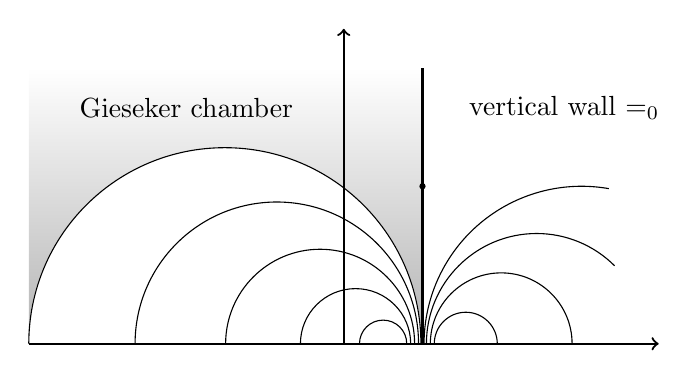
\begin{tikzpicture}

\shadedraw[bottom color=black!30!white,top color=white,draw=white] (-4,0) arc (180:0:2.49) -- (0,0) -- (1,0) -- (1,3.5) -- (-4,3.5);

\draw[thick,->] (-4,0) -- (4,0) node[anchor=south east] {$\be$};
\draw[thick,->] (0,0) -- (0,4) node[anchor=north west] {$\al$};

\draw[thick] (1,0) -- (1,3.5);


\draw[] (0.98,0) arc (0:180:2.49);
\draw[] (0.95,0) arc (0:180:1.8);
\draw[] (0.9,0) arc (0:180:1.2);
\draw[] (0.85,0) arc (0:180:0.7);
\draw[] (0.8,0) arc (0:180:0.3);

\draw[] (1.02,0) arc (180:80:2);
\draw[] (1.05,0) arc (180:45:1.4);
\draw[] (1.1,0) arc (180:0:0.9);
\draw[] (1.15,0) arc (180:0:0.4);

\draw (-2,3) node {Gieseker chamber};
\draw (2.8,3) node {vertical wall $\be = \be_0$};
\fill (1,2) circle (0.04) node[anchor=east] {$\si$};

\end{tikzpicture}
\end{center}
Our goal is to study the moduli space of semistable objects when $\si$ lies on the vertical wall.

\subsection{Stability on the vertical wall}\label{section:stabvertwall}
In this subsection we classify stable and semistable objects on the vertical wall. Let $v \in \Kn(X)$ be a class of positive rank, and let 
\[ (\Coh^{\be_0}(X), Z_{\al,\be_0}) \in \Stab(X) \] 
be the stability condition constructed in the previous section with 
\[ \be_0 = \frac{H \cdot \ch_1^B(v)}{H^2 \ch_0(v)} \quad \mathrm{and} \quad \al > 0. \] Note that since other walls do not intersect the vertical wall, the sets of stable and semistable objects are independent of $\al$.

We first note that there are no nonzero objects in $\Coh^{\be_0}(X)$ with numerical class $v$. Namely, by Lemma \ref{ss-ses}, any object $E \in \Coh^{\be_0}(X)$ with $\im Z_{\al,\be_0}(E) = 0$ fits in a triangle
\[ F[1] \to E \to T, \]
where $T$ has 0-dimensional support and $F$ is $\mu$-semistable. But $\rk(E) = \rk(T) + \rk(F[1]) = -\rk(F) \le 0$, while $\rk(v) > 0$ by assumption. Therefore, it is convenient to instead consider the stability condition 
\[ \si = (\sA, Z), \quad \mathrm{where} \quad \sA = \Coh^{\be_0}(X)[-1], \quad Z = -Z_{\al,\be_0}. \] 
Note that this does not change the slope function $\nu = -\re Z/\im Z$. By definition, the heart $\sA$ consists of objects $E$ with fitting in a triangle
\[ F \to E \to T[-1] \]
where $F \in \sF_{\be_0}, T \in \sT_{\be_0}$.

The next proposition gives a description of stable and semistable objects in $\sA$ of slope $\nu = \infty$ with respect to $\si$. This includes objects of class $v \in \Kn(X)$. Part (i) will be crucial in the proof that the moduli space $M^\si(v)$ of semistable objects of class $v$ is projective, and part (iii) will let us identify $M^\si(v)$ with the Uhlenbeck compactification of the moduli of $\mu$-stable vector bundles, at least on the level of points.
\begin{prop}\label{ss-object-vertical-classification}
    Let 
    \[ \si = (\sA, Z), \quad \mathrm{where} \quad \sA = \Coh^{\be_0}(X)[-1], \quad Z = -Z_{\al,\be_0}. \]
    \begin{enumerate}[(i)]
        \item Any object $E \in \sA$ with $\nu(E) = \infty$ is $\si$-{\bf semistable} and fits in a triangle
        \[ F \to E \to T[-1] \]
        where $T$ is a sheaf supported in dimension 0, and $F$ is a $\mu$-semistable sheaf of slope $\mu_B(F) = \be_0$. 
        \item An object $E \in \sA$ with $\nu(E) = \infty$ is $\si$-{\bf stable} if and only if in the above triangle either $F$ is a $\mu$-stable locally free sheaf and $T = 0$, or $T = \Oh_p$ is the structure sheaf of a closed point $p \in X$ and $F = 0$.
        \item An object $E \in \sA$ of class $v$ is $\si$-{\bf polystable} if and only if
        \[ E \cong \left(\bigoplus_i F_i\right) \oplus \left(\bigoplus_j \Oh_{p_j}[-1]\right), \]
        where each $F_i$ is a $\mu$-stable locally free sheaf of slope $\mu = \mu_B(v)$, and each $p_j \in X$ is a closed point.
    \end{enumerate}
\end{prop}
Part (i) of Proposition \ref{ss-object-vertical-classification} follows from Lemma \ref{ss-ses} and the constructions, while part (iii) follows from part (ii) by the definition of polystability. We prove part (ii)
in a series of lemmas below. Lemmas \ref{muStableLfIsSigmaStable} and \ref{skyscraperIsSigmaStable} show that $\mu$-stable locally free sheaves and shifted skyscraper sheaves are $\si$-stable, and Lemmas \ref{sigmaStablePosRkIsMuStable} and \ref{sigmaStableRk0isSkyscraper} show the converse.
\begin{lem}\label{muStableLfIsSigmaStable}
    A $\mu$-stable locally free sheaf $E$ with $\rk(E) > 0$ and $\mu_B(E) = \be_0$ is $\si$-stable.
\end{lem}
\begin{proof}
    Let $F \hookrightarrow E$ be an inclusion in $\sA$ with $\nu(F) = \infty$. We must show $F = 0$ or $F = E$. The induced short exact sequence
    \[ 0 \to F \to E \to G \to 0 \]
    is by definition an exact triangle in $D^b(X)$ with each vertex in $\sA$. Cohomology with respect to the standard t-structure leads to an exact sequence
    \[ 0 \to \sH^0(F) \to E \to \sH^0(G) \to \sH^1(F) \to 0 \to \sH^1(G) \to 0 \]
    of sheaves. This immediately implies that $\sH^1(G) = 0$, i.e. $G = \sH^0(G)$, and that $\sH^0(F)$ is a subsheaf of $E$.
    
    We have three cases.
    \begin{itemize}
        \item If $\sH^0(F) \xrightarrow{\sim} E$, then $G \xrightarrow{\sim} \sH^1(F)$. But $G \in \sF_{\be_0}, \sH^1(F) \in \sT_{\be_0}$, so we must have $G = \sH^1(F) = 0$, hence $F = \sH^0(F) = E$.
        
        \item If $\sH^0(F)$ is a proper, nonzero subsheaf of $E$, then by the assumption on $E$ we have $\mu_B(\sH^0(F)) < \mu_B(E) = \be_0$. Let $N$ denote the image of the map $E \to G$, so that we have the short exact sequences
        \[ 0 \to \sH^0(F) \to E \to N \to 0 \]
        and 
        \[ 0 \to N \to G \to \sH^1(F) \to 0. \]
        By assumption, $\nu(G) = \infty$ so $G$ is $\mu$-semistable, and thus $\mu_B(N) \le \mu_B(G)$. This gives the absurd inequality 
        \[ \be_0 = \mu_B(E) < \mu_B(N) \le \mu_B(G) \le \mu_B(\sH^1(F)) \le \be_0. \]
        Thus, this case is impossible.
        
        \item If $\sH^0(F) = 0$, then $F = \sH^1(F)[-1]$. Denote $F' = \sH^1(F)$. The short exact sequence
        \[ 0 \to E \to G \to F' \to 0 \]
        implies 
        \[ H\cdot \ch^B_1(G) = H\cdot \ch^B_1(E) + H\cdot \ch^B_1(F'). \]
        Assume for contradiction that $\rk(F') > 0$. Since $\rk(G) \ge \rk(E) > 0$ by assumption, from the above equality and the definition of $\mu_B$ we obtain
        \begin{align*} \be_0 \rk(E) + \mu_B(F') \rk(F') & = \mu_B(E) \rk(E) + \mu_B(F') \rk(F') \\
        & = \mu_B(G) \rk(G) \\
        & \le \be_0 \rk(G), \end{align*}
        so that
        \[ \mu_B(F') \rk(F') \le \be_0(\rk(G) -  \rk(E)) = \be_0 \rk(F'). \]
        However, since $\mu_B(F') > \be_0$, this inequality is impossible. Thus, $\rk(F') = 0$, which also implies $\rk(E) = \rk(G)$ and $\ch^B_1(F') = \ch_1(F')$. 
        
        Next, assume for contradiction that $F'$ has 1-dimensional support. Since $H$ is ample, this implies $H \cdot \ch^B_1(F') > 0$. But on the other hand, 
        \[ \mu_B(G) H^2 \rk(G) = \mu_B(E) H^2 \rk(E) + H \cdot \ch^B_1(F'), \]
        so that
        \[ H \cdot \ch^B_1(F') = H^2 (\mu_B(G) - \be_0)\rk(E) \le 0 \]
        since by assumption $\mu_B(G) \le \be_0$, again a contradiction. Thus, $F'$ has 0-dimensional support. Now if $F' \neq 0$, then we have a locally free subsheaf $E$ of a torsion-free sheaf $G$ with 0-di\-men\-sion\-al quotient $F'$. But as mentioned in \cite[Example 1.1.16]{HL}, the quotient $G/E$ has no 0-dimensional associated points. Thus, we must have $F' = 0$.
    \end{itemize} 
\end{proof}

\begin{lem}\label{skyscraperIsSigmaStable}
    The shifted skyscraper sheaf $\Oh_p[-1]$ is $\si$-stable for every closed point $p \in X$.
\end{lem}
\begin{proof}
    Let $F \hookrightarrow \Oh_p[-1]$ be an inclusion in $\sA$ with $\nu(F) = \infty$. We must show $F = 0$ or $F = \Oh_p[-1]$. Like above, the induced short exact sequence
    \[ 0 \to F \to \Oh_p[-1] \to G \to 0 \]
    in $\sA$ yields the exact sequence
    \[ 0 \to \sH^0(G) \to F \to \Oh_p \to \sH^1(G) \to 0 \]
    of sheaves, and $F = \sH^1(F)$. If $\Oh_p \xrightarrow{\sim} \sH^1(G)$, then $\sH^0(G) \cong F$, and since $\sH^0(G) \in \sF_\be, F \in \sT_\be$, we have $F = 0$.
    
    If on the other hand $\sH^1(G) = 0$, then $G = \sH^0(G)$, and the short exact sequence
    \[ 0 \to G \to F \to \Oh_p \to 0 \]
    implies that $\mu_B(G) = \mu_B(F)$, and we once again see that $G = F = 0$, a contradiction.
\end{proof}

%mmmmmme....................rrrrrrrrrrrrrrrr        <------ Fennel, July 8, 2020. (Fennel is a two-month old kitten.)

\begin{lem}\label{sigmaStablePosRkIsMuStable}
    If $E \in \sA$ is a $\si$-stable object with $\rk(E) > 0$ and $\nu(E) = \infty$, then $E$ is a $\mu$-stable locally free sheaf.
\end{lem}
\begin{proof}
    The object $E$ fits in an exact triangle
    \[ F \to E \to T[-1] \]
    where $F$ is a $\mu$-semistable torsion-free sheaf with $\mu_B(F) = \be_0$ and $T$ is a 0-dimensional sheaf. If $T \neq 0$, then $F$ is a destabilizing subobject of $E$ in $\sA$ unless $F = 0$, in which case $\rk(E) = -\rk(T) = 0$, contrary to the assumption. Thus, $T = 0$ and $E$ is a $\mu$-semistable sheaf.
    
    We next show that $E$ is locally free. Since $E$ is torsion-free, the canonical evaluation map $E \to E^{\vee \vee}$ is injective with cokernel $Q$ supported in dimension 0. Now $E^{\vee\vee}$ and $Q[-1]$ both lie in the heart $\sA$, so the short exact sequence 
    \[ 0 \to E \to E^{\vee \vee} \to Q \to 0 \]
    of coherent sheaves gives an exact sequence
    \[ 0 \to Q[-1] \to E \to E^{\vee \vee} \to 0 \]
    in $\sA$. Since $\nu(Q[-1]) = \nu(E) = \infty$ and $E$ is stable, we must have $Q = 0$, and so $E \cong E^{\vee\vee}$ is locally free.
    
    To show that $E$ is $\mu$-stable, let
    \[ 0 \subset E_1 \subset \cdots \subset E_r = E \]
    be a Jordan-H\"older filtration into $\mu$-stable factors. If $r > 1$, then $E/E_1$ is a $\mu$-semistable sheaf with $\mu_B(E/E_1) = \be_0$, so the short exact sequence of sheaves
    \[ 0 \to E_1 \to E \to E/E_1 \to 0 \]
    is also a short exact sequence in $\sA$ of objects with $\nu = \infty$, which contradicts the $\si$-stability of $E$. Thus, $E = E_1$ is $\mu$-stable.
\end{proof}

\begin{lem}\label{sigmaStableRk0isSkyscraper}
    If $E \in \sA$ is $\si$-stable with $\rk(E) = 0$ and $\nu(E) = \infty$, then $E = \Oh_p[-1]$ for some closed point $p \in X$.
\end{lem}
\begin{proof}
    From the triangle
    \[ F \to E \to T[-1] \]
    as above, we get 
    \[ 0 = \rk(E) = \rk(F) - \rk(T) = \rk(F), \]
    so since $F$ is torsion-free, we must have $F = 0$, and $E = T[-1]$ is the shift of a 0-dimensional sheaf. But any proper subsheaf $T' \subs T$ is also 0-dimensional, so $T'[-1] \in \sA$ is a destabilizing subobject of $E$ with respect to $\si$. Thus, $T$ must have length 1, and so $T = \Oh_p$ for some $p \in X$.
\end{proof}

\begin{rmk}
Proposition \ref{ss-object-vertical-classification} can also be deduced from \cite[Proposition 2.2]{huy} as follows. Any stable object $E \in \sA$ is minimal, since a nonzero surjection $E \twoheadrightarrow E'$ in $\sA$ implies $\nu(E') > \nu(E)$ unless $E' = E$. Conversely any minimal object is automatically stable. Although \cite[Proposition 2.2]{huy} is stated in the case when $X$ is a K3 surface, the proof works for any surface.
\end{rmk}

%%%%%%%%%%%%%%%%%%%%%%%%%%%%%%%%%%%%%%%%%%%%%
%%%%%%  MODULI OF SEMISTABLE OBJECTS  %%%%%%%
%%%%%%%%%%%%%%%%%%%%%%%%%%%%%%%%%%%%%%%%%%%%%

\section{Moduli of semistable objects}\label{section:moduliofbridgeland}
In this section we overview some definitions and results regarding moduli spaces of Bridgeland semistable objects. 

\subsection{Moduli stacks}
Let $X$ be a smooth, projective surface over $\C$ with a very ample divisor $H$, let $v \in \Kn(X)$ be a numerical class, and let $\si = (\sA, Z) \in \Stab(X)$ be a Bridgeland stability condition on $X$. Define a category fibered in groupoids $\sM^\si(v)$ over the big \'etale site of $\C$-schemes as follows. The objects of $\sM^\si(v)$ are pairs $(S, \sE)$, where $S$ is a scheme over $\C$, and $\sE \in D^b(S \times X)$ is a complex of coherent sheaves relatively perfect over $S$, and whenever $S$ is of finite type over $\C$, for every closed point $s \in S$, the derived restriction of $E$ to the fiber $\{s\} \times X \cong X$ lies in $\sA$, is $\si$-semistable, and has numerical class $v$. A morphism $(S', \sE') \to (S, \sE)$ in $\sM^\si(v)$ is a pair $(f, f^\sharp)$, where $f: S' \to S$ is a morphism of $\C$-schemes, and $f^\sharp: \sE \to f_* \sE'$ is a morphism in $D^b(S \times X)$ whose adjoint is an isomorphism $f^* \sE \xrightarrow{\sim} \sE'$ in $D^b(S' \times X)$.

If $\si$ is obtained by tilting with respect to $\mu$-stability as in Section \ref{section:stabcondsurf}, then based on work in \cite{lie06}, \cite{ABL13}, and \cite{AP06}, it is proved in \cite{toda08} that $\sM^\si(v)$ is an algebraic stack of finite type over $\C$. 

\subsection{Good moduli spaces}
Recall that if $\sM$ is an algebraic stack, a quasi-compact, quasi-separated morphism $\pi: \sM \to M$ to an algebraic space $M$ is called a {\bf good moduli space}, if the pushforward functor $\pi_*: \Qcoh(\sM) \to \Qcoh(M)$ is exact, and the natural map $\Oh_M \to \pi_*\Oh_\sM$ is an isomorphism.

In \cite{AHLH}, the authors give necessary and sufficient conditions for the existence of a good moduli space in terms of certain valuative criteria. As an application, the authors construct proper good moduli spaces for various moduli stacks $\sM^{\mathrm{ss}}_\sA$ parameterizing objects in an abelian category $\sA$ that are semistable with respect to a rather general notion of stability on $\sA$. This construction includes stacks of Bridgeland semistable objects on a smooth, projective variety $X$ with respect to a numerical stability condition $\si = (\sA, Z) \in \Stab(X)$ whose heart $\sA$ is noetherian and satisfies the ``generic flatness property'', and for which the moduli stacks $\sM^\si(v)$ are of finite type. See \cite[Section 7]{AHLH} for details, especially Theorem 7.25 and Example 7.27. In particular, we have the following.
\begin{thm}\label{gmsexists}
    Let $X$ be a smooth, projective surface over $\C$, let $v \in \Kn(X)$ be a numerical class, and let $\si \in \Stab(X)$ be a stability condition constructed by tilting with respect to slope-stability as in Section \ref{section:stabcondsurf}. The moduli stack $\sM^\si(v)$ of $\si$-semistable objects of class $v$ admits a good moduli space map $\sM^\si(v) \to M^\si(v)$, where $M^\si(v)$ is a proper algebraic space over $\C$. The closed points of $M^\si(v)$ are in bijection with S-equivalence classes of $\si$-semistable objects of class $v$.
\end{thm}



%%%%%%%%%%%%%%%%%%%%%%%%%%%%%%%%%%%%%%%%%%%%%
%%%%%%%%%%%%%  NEF LINE BUNDLE  %%%%%%%%%%%%%
%%%%%%%%%%%%%%%%%%%%%%%%%%%%%%%%%%%%%%%%%%%%%

\section{The nef line bundle}
In \cite{BM}, the authors construct a natural numerical class of line bundles with strong positivity properties on a Bridgeland moduli space $\sM^\si(v)$ that varies with the stability condition $\si$. We recall here the construction and basic properties of the line bundle, as well as identify the line bundle on the vertical wall.

\subsection{Definition and positivity properties}\label{positiveLBdefandprops}
Let $(X,H)$ be a smooth, projective, polarized surface, let $\si = (\sA, Z) \in \Stab(X)$ be a stability condition, and let $v \in \Kn(X)$ be a numerical class. Assume that the moduli stack $\sM^\si(v)$ of $\si$-semistable objects in $\sA$ of class $v$ is algebraic, and denote by $\sE$ the universal complex on $\sM^\si(v) \times X$. Consider the following diagram:
\begin{center}
    \begin{tikzpicture}
    \matrix (m) [matrix of math nodes, row sep=1.5em, column sep=1em]
    { & \sM^\si(v) \times X & \\
    \sM^\si(v) & & X \\};
    \path[->] 
    (m-1-2) edge node[auto,swap] {$ p $} (m-2-1)
    (m-1-2) edge node[auto] {$ q $} (m-2-3)
    ;
    \end{tikzpicture}
\end{center}
The Donaldson morphism
\[ \la_\sE: K_0(X) \to \Pic(\sM^\si(v)), \quad [F] \mapsto \det R p_*(\sE \otimes q^* F) \]
from Section \ref{section:determinantal} induces a map 
\[ \la_\sE: \Kn(X)_\R \to \Num(\sM^\si(v))_\R. \]
Define a real divisor class on $\sM^\si(v)$ by applying the Donaldson morphism to the unique class $w_Z \in \Kn(X)_\R$ determined by the condition
\[ \chi(w_Z, -) = \im\left(-\frac{Z(-)}{Z(v)}\right). \]
This condition indeed defines a unique class since the Euler pairing $\chi(-,-)$ induces a perfect pairing on $\Kn(X)_\R$. Denote this numerical class by $\sL_\si \coloneqq \la_\sE(w_Z)$. The following is \cite[Lemma 3.3]{BM}, and it is the main result of the paper.
\begin{thm}\label{BMpositivity}
    Let $C$ be a projective, integral curve over $\C$, and let $f: C \to \sM^\si(v)$ be a morphism.
    \begin{enumerate}[(1)]
        \item $\deg f^* \sL_\si \ge 0$.
        \item If $\deg f^* \sL_\si = 0$, then for any two closed points $s, t \in C$, the objects \\ $(f \times \id_X)^*\sE|_{\{s\} \times X}$ and $(f\times \id_X)^*\sE|_{\{t\} \times X}$ are S-equivalent.
    \end{enumerate}
\end{thm}
In \cite{BM}, part (2) is stated so that the objects $(f \times \id_X)^*\sE|_{\{t\} \times X}$ are S-equivalent for points $t$ in some nonempty open subscheme $U \subs C$. We deduce the above statement from Theorem \ref{gmsexists} as follows. If $\sM^\si(v) \to M^\si(v)$ denotes the good moduli space map, then the composition $C \to \sM^\si(v) \to M^\si(v)$ maps the dense open set $U$ to a point, hence must be constant, and so the objects $(f\times \id_X)^*\sE|_{\{t\} \times X}$ are all S-equivalent. 

We would like to know that the real divisor class $\sL_\si$ descends to the good moduli space $M^\si(v)$. In \cite{BM} and \cite{nuer} this is done using a so-called quasi-universal family on the stable locus of the moduli space. However, we can achieve this on all of $M^\si(v)$ as follows.
\begin{lem}\label{nefdescendtogms}
    If $w \in K(X)$ is a class whose image in $\Kn(X)_\R$ is a multiple of $w_Z$, then $\la_\sE(w)$ descends to the good moduli space $M^\si(v)$.
\end{lem} 
\begin{proof}
    Write $w = b w_Z$ in $\Kn(X)_\R$ with $b \in \R$. We check the condition in Proposition \ref{lbtogms}. If $E \cong E_1^{\oplus r_1} \oplus \cdots \oplus E_m^{\oplus r_m}$ is a $\si$-polystable object of class $v$, then for each $i$, the complex number $Z(E_i)$ lies on the same ray as $Z(E)$, so that $Z(E_i)/Z(v)$ is real, and so
    \[ \chi(w, E_i) = b\,\chi(w_Z, E_i) = b\,\im\left(-\frac{Z(E_i)}{Z(v)}\right) = 0. \]
    Thus, $\la_\sE(w)$ descends to a line bundle on the good moduli space.    
\end{proof}
This lets us define a numerical class $L_\si$ on $M^\si(v)$ by setting $L_\si = \frac{1}{b}[\sN]$ where $\pi^*\sN = \la_\sE(w)$ such that $w \in K(X)$ satisfies $w \equiv b w_Z$ in $\Kn(X)$ and $b > 0$. The class $L_\si$ is independent of the choice of $w$. We would like to know that $L_\si$ enjoys the same positivity properties as $\sL_\si$.
\begin{lem}\label{gmsnef}
    Let $C$ be a smooth, projective, integral curve over $\C$, and let $g: C \to M^\si(v)$ be a morphism.
    \begin{enumerate}[(1')]
        \item $\deg g^* L_\si \ge 0$.
        \item If $\deg g^* L_\si = 0$, then $g$ is constant.
    \end{enumerate}
\end{lem}
\begin{proof}
    By Lemma \ref{finitecurveextension}, we can find a commutative diagram
    \begin{center}
    \begin{tikzpicture}
    \matrix (m) [matrix of math nodes, row sep=2em, column sep=2em]
    { C' & \sM^\si(v)  \\
    C & M^\si(v) \\};
    \path[->] 
    (m-1-1) edge node[auto] {$ f $} (m-1-2)
    (m-1-1) edge node[auto,swap] {$ \phi $} (m-2-1)
    (m-1-2) edge node[auto] {$ \pi $} (m-2-2)
    (m-2-1) edge node[auto,swap] {$ g $} (m-2-2)
    ;        
    \end{tikzpicture}
    \end{center}
    where $C'$ is a smooth, projective curve, $\phi$ is a finite morphism, and $\pi$ is the good moduli space map. To prove (1') we note that
    \[ \deg(\phi) \deg g^* L_\si = \deg (g \circ \phi)^* L_\si = \deg(\pi \circ f)^* L_\si = \deg f^*\sL_\si \ge 0, \]
    so since $\deg(\phi) > 0$, we get $\deg g^* L_\si \ge 0$.
    
    To prove (2'), assume that $\deg g^*L_\si = 0$. Then also $f^* \sL_\si = 0$, so by part (2) of Theorem \ref{BMpositivity}, the family parameterized by $C'$ consists of S-equivalent objects, so the composition $\pi \circ f: C' \to M^\si(v)$ maps every closed point of $C'$ to the same point $p_0 \in |M^\si(v)|$, and the same holds for $g: C \to M^\si(v)$, and so the scheme-theoretic image of $g$ is a closed point of $M^\si(v)$.
\end{proof}


\subsection{The nef line bundle on the vertical wall}
We can describe the class $w_Z \in \Kn(X)$ more explicitly in the case of the stability condition 
\[ \si = (\sA, Z) = (\Coh^{\be_0}(X)[-1], -Z_{\al, \be_0}), \quad \mathrm{where} \quad \be_0 = \frac{H \cdot \ch_B^1(v)}{H^2 \ch_B^0}, \; \al > 0, \] that is, when $\si$ lies on the vertical wall for $v$. Recall that $H \subs X$ denotes a fixed very ample divisor. Denote $h = [\Oh_H] \in K(X)$.
\begin{propdef}\label{nefclassonverticalwall}
    Let $(X,H)$ be a smooth, projective, polarized surface, let $v \in \Kn(X)$ be a class of positive rank, and let $\si \in \Stab(X)$ lie on the vertical wall for $v$ as in Section \ref{section:stabvertwall}. Define 
    \[ u = -\chi(v \cdot h^2) h + \chi(v \cdot h) h^2 \in K(X). \]
    We have 
    \[ w_Z = -\frac{\al}{\rk(v) Z(v) \deg X} u. \]
\end{propdef}
Note that $Z(v)$ is a negative real number, so $w_Z$ is indeed a positive multiple of $u$. Thus, $\la_\sE(u)$ enjoys the same positivity properties as $\sL_\si = \la_\sE(w_Z)$.
\begin{proof}
    Fix a closed point $p \in X$, and denote the numerical Todd class of $X$ by
    \[ \td_X = 1 - \frac{1}{2} K_X + \chi(\Oh_X) [p]. \]
    We will use the Hirzebruch-Riemann-Roch formula:
    \[ \chi(a \cdot b) = \int_X \ch(a) \ch(b) \td_X \]
    for $a, b \in \Kn(X)$.
    
    Let $a \in K(X)$ be arbitrary. To compute $\chi(a \cdot u)$, we may replace $u$ with something numerically equivalent. Now $h^2 \equiv \deg(X) [\Oh_p]$ by Bertini, and $v \cdot [\Oh_p] = \rk(v)$, so if we set
    \[ u' = - \rk(v) h + \chi(v \cdot h) [\Oh_p] \]
    we can consider the class $\deg(X) u'$ instead of $u$. Moreover, 
    \[ \ch(\Oh_H) = \ch(\Oh_X) - \ch(\Oh_X(-H)) = H - \frac{1}{2} H^2, \quad \ch(\Oh_p) = [p], \]
    so by Hirzebruch-Riemann-Roch,
    \begin{align*}
        \chi(v \cdot h) & = \int_X (\rk(v) + \ch_1(v))\left(H - \frac{1}{2}H^2\right)\left(1 - \frac{1}{2}K_X\right) \\
        & = \ch_1(v) \cdot H - \frac{\rk(v)}{2} H\cdot(H + K_X),
    \end{align*}
    and hence
    \begin{align*}
        \ch(u') & = -\rk(v) \ch(\Oh_H) + \chi(v \cdot [\Oh_H]) \ch(\Oh_p) \\
        & = -\rk(v)\left(H - \frac{1}{2}H^2\right) + \left(\ch_1(v) \cdot H - \frac{\rk(v)}{2} H(H + K_X)\right)[p] \\
        & = -\rk(v) H + \left(\ch_1(v) \cdot H - \frac{\rk(v)}{2} H \cdot K_X\right)[p]
    \end{align*}
    Since $\ch(u')$ is in $A^{\ge 1}(X)$, we only need to know the $A^{\le 1}(X)$-part of $\ch(a)\td_X$, which is
    \[ \ch(a) \td_X = (\ch_0(a) + \ch_1(a)) (1 - \frac{1}{2} K_X) \equiv \ch_0(a) - \frac{1}{2} \ch_0(a) K_X + \ch_1(a). \]
    Putting everything together, we now calculate
    \begin{align*}
        \chi(a \cdot u') & = \int_X \ch(a) \ch(u') \td_X \\
        & = \int_X \left(\ch_0(a) - \frac{1}{2} \ch_0(a) K_X + \ch_1(a)\right)\cdot  \\
        & \quad\left(-\ch_0(v) H + \ch_1(v) H - \frac{1}{2} \ch_0(v) H \cdot K_X\right) \\
        & = H \cdot (\ch_0(a) \ch_1(v) - \ch_0(v) \ch_1(a)) \\
        & = H \cdot (\ch^B_0(a) \ch^B_1(v) - \ch^B_0(v) \ch^B_1(a))
    \end{align*}
    Thus,
    \[ \chi(a \cdot u) = \deg X \cdot \chi(a \cdot u') = \deg X \cdot H (\ch^B_0(a) \ch^B_1(v) - \ch^B_0(v) \ch^B_1(a)). \]
    
    Next we calculate $\im(-Z(a)/Z(v))$. Recall that since $\si$ is on the vertical wall for $v$, the quantity $Z(v)$ is a negative real number, and so 
    \[ \im\left(-\frac{Z(a)}{Z(v)}\right) = -\frac{1}{Z(v)} \im Z(a). \]
    Now 
    \begin{align*}
        \im Z(a) & = \al(\be_0 H^2 \ch^B_0(a) - H \cdot \ch^B_1(a)) \\
        & = \al \left( \frac{H \cdot \ch^B_1(v)}{H^2 \ch^B_0(v)} H^2 \ch^B_0(a) - H \cdot \ch^B_1(a) \right) \\
        & = \frac{\al}{\ch^B_0(v)} H (\ch^B_0(a) \ch^B_1(v) - \ch^B_0(v) \ch^B_1(u)).
    \end{align*}
    Thus, we see that
    \[ \im\left(-\frac{Z(a)}{Z(v)}\right) = -\frac{\al}{\rk(v) Z(v) \deg X} \chi(a \cdot u). \]
\end{proof}

\begin{rmk}
    The calculation of $w_Z$ as in Proposition \ref{nefclassonverticalwall} appears in \cite{liuwanmin} using a dual version of the Donaldson morphism. See in particular \cite[Theorem 4.13(b)]{liuwanmin}
\end{rmk}



%%%%%%%%%%%%%%%%%%%%%%%%%%%%%%%%%%%%%%%%%%%%%
%  PROJECTIVITY OF THE GOOD MODULI SPACE  %%
%%%%%%%%%%%%%%%%%%%%%%%%%%%%%%%%%%%%%%%%%%%%%
\section{Projectivity of the good moduli space}

Let $(X, H)$ be a smooth, projective, polarized surface over $\C$, let $v \in \Kn(X)$ be a nu\-mer\-i\-cal class with $\rk(v) > 0$, and let $\si$ be a stability condition lying on the vertical wall for $\si$ considered in Section \ref{section:stabvertwall}, that is,
\[ \si = (\sA, Z) = (\Coh^{\be_0}(X)[-1], -Z_{\al, \be_0}), \quad \mathrm{where} \quad \be_0 = \frac{H \cdot \ch_B^1(v)}{H^2 \ch_B^0}, \; \al > 0. \]
Let $\sM^\si(v)$ be the stack of $\si$-semistable objects of class $v$ in $\sA$, and let $\sE$ be the universal complex on $\sM^\si(v) \times X$. In this section we prove that the good moduli space $M^\si(v)$ of the stack $\sM^\si(v)$ is projective. 

Recall from Section \ref{positiveLBdefandprops} that $\sL_\si$ denotes the natural nef line bundle on $\sM^\si(v)$ and $L_\si$ the corresponding line bundle on $M^\si(v)$. We will show that $L_\si$ is ample. Since by Lemma \ref{nefdescendtogms}, $L_\si$ is strictly positive on any proper curve in $M^\si(v)$, it suffices to show that $L_\si$ is semiample, meaning that some tensor power is globally generated. Moreover, since by Proposition \ref{vbtogms}, sections of $\sL_\si$ descend to sections of $L_\si$, it suffices to show that $\sL_\si$ is semiample. To produce sections of $\sL_\si$, we expand on techniques used in \cite{li} for constructing a scheme structure on the Uhlenbeck compactification, and in \cite{seshadri} for constructing moduli spaces of vector bundles on a curve. 

The idea is as follows. First, we explain how to obtain a diagram
\begin{center}
    \begin{tikzpicture}
    \matrix (m) [matrix of math nodes, row sep=3em, column sep=0.5em]
    { & \sM^\si(v) \times X & & \sM^\si(v) \times C & \\
    \sM^\si(v) & & X & & C \\};
    \path[left hook->] 
    (m-1-4) edge node[auto,swap] {$ j $} (m-1-2)
    (m-2-5) edge node[auto] {$ i $} (m-2-3)
    ;
    \path[->]
    (m-1-2) edge node[auto,swap] {$ p $} (m-2-1)
    (m-1-2) edge node[pos=0.9,yshift=10pt] {$ q $} (m-2-3)
    (m-1-4) edge node[pos=0.7,yshift=-8pt] {$ p_C $} (m-2-1)
    (m-1-4) edge node[auto] {$ q_C $} (m-2-5)
    ;        
    \end{tikzpicture}
\end{center}
where $C$ is a smooth curve in the linear system $|a H|$ for $a > 0$, together with a locally free sheaf $G$ on $C$, with the property that the determinantal line bundle
\[ \la_{j^* \sE}(G)^\vee = \det(R p_{C*}(j^*\sE \otimes q_C^*G))^\vee \]
is a positive multiple of $\sL_\si$ on $\sM^\si(v)$. 

Next, by analyzing restrictions of $\si$-semistable objects $E$ to $C$, we apply Lemma \ref{detsection}(a) to show that $\la_{j^* \sE}(G)^\vee$ has a canonical global section $\de_G$ on $\sM^\si(v)$. Moreover, we show that for a given $\C$-point $t \in \sM^\si(v)$, we can choose the curve $C$ and the sheaf $G$ so that the section $\de_G$ is nonvanishing at $t$. To do this, recall from Proposition \ref{ss-object-vertical-classification} that the complex $\sE_t$ on $\{t\} \times X = X$ fits in an exact triangle
\[ F \to \sE_t \to T[-1] \]
in $D^b(X)$, where $F$ is a $\mu$-semistable torsion-free sheaf and $T$ is a torsion sheaf with 0-dimensional support. Using a restriction theorem for $\mu$-stability, we show that we can choose $a \gg 0$ and $C \in |a H|$ so that
\begin{enumerate}[(1)]
    \item $C$ avoids the support of $T$, and
    \item the restriction $\sE_t|_C = F|_C$ to $C$ is slope-semistable.
\end{enumerate}
Using a characterization of semistability on a curve due to Faltings and Seshadri, we find a locally free sheaf $G$ on $C$ with the property that 
\[ H^0(C, F|_C \otimes G) = H^1(C, F|_C \otimes G) = 0, \]
and apply Lemma \ref{detsection}(b) to translate this into the nonvanishing of $\de_G$ at $t$.

Finally, by varying $C$ and $G$, we produce a generating set of sections of some power of $\sL_\si$, or equivalently $L_\si$, and use Theorem \ref{gmsexists} and Lemma \ref{gmsnef} to show that the morphism $M^\si(v) \to \p^N$ induced by the sections is finite. From this we conclude that $M^\si(v)$ is projective.

\subsection{Sheaves on curves and the nef line bundle}
We begin to carry out the plan outlined above. To set up some notation, let $C \subs X$ be a smooth, connected curve in the linear system $|a H|$ for some $a > 0$, and consider the diagram:
\begin{center}
    \begin{tikzpicture}
    \matrix (m) [matrix of math nodes, row sep=3em, column sep=0.5em]
    { & \sM^\si(v) \times X & & \sM^\si(v) \times C & \\
    \sM^\si(v) & & X & & C \\};
    \path[left hook->] 
    (m-1-4) edge node[auto,swap] {$ j $} (m-1-2)
    (m-2-5) edge node[auto] {$ i $} (m-2-3)
    ;
    \path[->]
    (m-1-2) edge node[auto,swap] {$ p $} (m-2-1)
    (m-1-2) edge node[pos=0.9,yshift=10pt] {$ q $} (m-2-3)
    (m-1-4) edge node[pos=0.7,yshift=-8pt] {$ p_C $} (m-2-1)
    (m-1-4) edge node[auto] {$ q_C $} (m-2-5)
    ;        
    \end{tikzpicture}
\end{center}
where $p, q, p_C, q_C$ denote the projections, and $i$ and $j$ are closed embeddings. Let $\sE_C \coloneqq j^*\sE$ be the restriction of $\sE$ to $\sM^\si(v) \times C$, which is perfect relative to $\sM^\si(v)$. We have the Donaldson homomorphisms
\[ \la_\sE: K(X) \to \Pic(\sM^\si(v)), \quad \la_{\sE_C}: K(C) \to \Pic(\sM^\si(v)). \]
In addition, for any $n \in \Z$, we have a map $K(X) \to K(X), w \mapsto w(n)$ induced by the map on locally free sheaves $F \mapsto F(n) = F \otimes \Oh_X(n)$. Similarly we have a map $K(X) \to K(C), w \mapsto w|_C$ induced by $F \mapsto F|_C = i^*F$. We denote $h = [\Oh_H] \in K(X)$ as before.

Recall from Proposition \ref{nefclassonverticalwall} that for the class 
\[ u = -\chi(v \cdot h^2) h + \chi(v \cdot h) h^2 \in K(X), \]
the line bundle $\la_\sE(u)$ on $\sM^\si(v)$ is a positive multiple of the natural nef line bundle $\sL_\si$. We first establish the following.
\begin{propdef}\label{nefpowerfromcurves}
    Given an integer $a > 0$ and a smooth, connected curve $C \in |a H|$, define the class
    \[ w \coloneqq -\chi(v \cdot h \cdot [\Oh_C]) \cdot 1 + \chi(v \cdot [\Oh_C]) \cdot h \in K(X). \]
    We have an isomorphism
    \[ \la_{\sE_C}(w|_C) \cong \la_\sE(u)^{a^2}. \]
    Moreover, the class $-w|_C \in K(C)$ has positive rank, and so can be represented by a locally free sheaf $G$ on $C$.
\end{propdef}

The proof of the following simple lemma as well as part of the proof of Proposition \ref{nefpowerfromcurves} below are essentially included in the proof of \cite[Proposition 8.2.3]{HL}.

\begin{lem}\label{Ktheorylemma}
    If $C \in |a H|$ is a curve and $w' \in K(X)$ is arbitrary, then
    \[ \la_\sE(w' - w'(-a)) = \la_{\sE_C}(w'|_C). \]
\end{lem}
\begin{proof}
    Both sides of the equation are linear in $w'$, so it suffices to consider the class $w' = [F]$ for a locally free sheaf $F$ on $X$. On the one hand, we have
    \begin{align*}
        \la_{\sE_C}(F|_C) & = \det R p_{C*}(\sE_C \otimes q_C^* i^* F) \\
        & = \det R p_* j_*(\sE_C \otimes j^* q^* F) \\
        & = \det R p_* (j_*\sE_C \otimes q^* F). \qquad \mathrm{(projection\;formula)}
    \end{align*}
    On the other hand, pulling back the short exact sequence 
    \[ 0 \to \Oh_X(-a) \to \Oh_X \to j_* \Oh_C \to 0 \]
    along $q$, tensoring with $\sE \otimes q^* F$, and applying $R p_*$ gives the exact triangle
    \[ R p_* (\sE \otimes q^*(F \otimes \Oh_X(-a))) \to R p_* (\sE \otimes q^*F) \to R p_* (j_* \sE_C \otimes q^*F) \]
    in $D^b(\sM^\si(v))$, and so we obtain an isomorphism
    \[ \det R p_* (j_* \sE_C \otimes q^*F) \cong \la_\sE(F) \otimes \la_\sE(F(-a))^\vee = \la_\sE(w - w(-a)). \]
\end{proof}

\begin{proof}[Proof of Proposition \ref{nefpowerfromcurves}]
    By Lemma \ref{Ktheorylemma}, for the first statement it is enough to show that
    \[ w - w(-a) = a^2 u. \]
    Since $[\Oh_X(-1)] = 1 - h \in K(X)$, we have
    \[ [\Oh_X(-a)] = [\Oh_X(-1)]^a = (1 - h)^a = 1 - a h + \binom{a}{2} h^2, \]
    so the short exact sequence
    \[ 0 \to \Oh_X(-a) \to \Oh_X \to \Oh_C \to 0 \]
    gives $[\Oh_C] = 1 - [\Oh_X(-a)] = a h - \binom{a}{2} h^2$. In particular, $h \cdot [\Oh_C] = a h^2$. We now calculate
    \begin{align*}
        w - w(-a) & = w \cdot [\Oh_C] \\
        & = (-\chi(v \cdot h \cdot [\Oh_C]) \cdot 1 + \chi(v \cdot [\Oh_C]) \cdot h) (a h - \binom{a}{2} h^2) \\
        & = - \chi(v \cdot ah^2) (a h - \binom{a}{2} h^2) + \chi\left(v \cdot (a h - \binom{a}{2} h^2)\right) a h^2 \\
        & = a^2 ( - \chi(v \cdot h^2) h + \chi(v \cdot h) h^2) = a^2 u.
    \end{align*}
    For the second claim, we note that 
    \[ -w|_C = \chi(v|_C \cdot h|_C) \cdot 1 - \chi(v|_C) \cdot h|_C = a \rk(v) \deg X \cdot 1 - \chi(v|_C) \cdot h|_C, \]
    and so 
    \[ \rk(w|_C) = a \rk(v) \deg X \rk(1) - \chi(v|_C) \rk(h|_C) = a \rk(v) \deg(X) > 0. \] 
    Since $C$ is smooth, projective, and connected, the natural map 
    \[ K(C) \to \Z \oplus \Pic(C), \quad [F] \mapsto (\rk F, \det F) \] 
    is an isomorphism. Moreover, any class $(m, L) \in \Z \oplus K(C)$ with $m > 0$ can be represented by a locally free sheaf: take for instance $G = \Oh_C^{\oplus m-1} \oplus L$. In particular, there exist locally free sheaves $G$ of class $- w|_C$ on $C$.
\end{proof}

\subsection{Producing sections}
Our next task is to show that the construction of Proposition \ref{nefpowerfromcurves} yields a canonical section $\de_G$ of the line bundle $\la_{\sE_C}(G)^\vee \cong \la_\sE(u)^{m a^2}$ on $\sM^\si(v)$, and that by choosing $C$ and $G$ carefully, this section is nonzero at a given point $t \in \sM^\si(v)$. After some preparations, we prove this in Proposition \ref{globalgen}. In the proof, Lemmas \ref{restsingle} and \ref{hypercohovanishing} will be used to apply Lemma \ref{detsection}(a), and Lemmas \ref{restsemistable} and \ref{seshadrimainlemma1} to apply Lemma \ref{detsection}(b).

\begin{lem}\label{restsingle} 
    Let $X$ be a smooth, projective surface and $C \subs X$ a smooth, projective curve. Assume $E \in D^b(X)$ fits in a triangle
    \[ F \to E \to T[-1], \]
    where $F$ is a torsion-free sheaf and $T$ is a torsion sheaf with 0-di\-men\-sion\-al support. The derived restriction $E|_C^\LL$ fits in a triangle
    \[ \sH^0(E|_C^\LL) \to E|_C^\LL \to \sH^1(E|_C^\LL)[-1] \]
    in $D^b(C)$, where $\sH^1(E|_C^\LL)$ is a torsion sheaf.
\end{lem}
\begin{proof}
Derived restriction to $C$ is a functor of triangulated categories, so we obtain a triangle
\[ F|_C^\LL \to E|_C^\LL \to T|_C^\LL[-1], \]
which yields a long exact sequence of cohomology sheaves
\[ \cdots \to \sH^i(F|_C^\LL) \to \sH^i(E|_C^\LL) \to \sH^i(T|_C^\LL[-1]) \to \sH^{i+1}(F|_C^\LL) \to \cdots. \]
To understand the terms in this sequence, we study the derived restrictions $F|_C^\LL$ and $T|_C^\LL$. Since pushforward of coherent sheaves along the inclusion $C \hookrightarrow X$ is exact, we may as well study the derived tensor products $F \otimes^\LL \Oh_C$ and $T \otimes^\LL \Oh_C$, where $\Oh_C$ is the structure sheaf of $C$ viewed as an $\Oh_X$-module. 

Since $C \subs X$ is a Cartier divisor, $\Oh_C$ has a resolution by line bundles
\[ 0 \to \Oh_X(-C) \xrightarrow{f} \Oh_X \to \Oh_C \to 0. \]
Thus, the objects $F \otimes^\LL \Oh_C$ and $T \otimes^\LL \Oh_C$ are represented by the complexes
\[ \sF = [F(-C) \xrightarrow{f} F] \qquad \mathrm{and} \qquad \sT = [T(-C) \xrightarrow{f} T] \]
respectively, where $F$ and $T$ are placed in degree 0. 


Since $F$ is by assumption torsion-free, the map $f: F(-C) \to F$ is injective. Thus, we see that $\sH^0(F|_C^\LL) = \sH^0(\sF) = F|_C$ agrees with the ordinary restriction, and $\sH^i(F|_C^\LL) = \sH^i(\sF) = 0$ for $i \neq 0$. Moreover, from $\sT$ we see that $\sH^{-1}(T|_C^\LL) = \sH^{-1}(\sT)$ is a subsheaf of $T(-C) \cong T$, and $\sH^0(T|_C^\LL) = \sH^0(\sT)$ is a quotient of $T$, hence both are 0-dimensional, and $\sH^i(T|_C^\LL) = 0$ for $i \neq -1, 0$.

We now return to the triangle
\[ F|_C^\LL \to E|_C^\LL \to T|_C^\LL[-1] \]
at the beginning of the proof. Taking into account the shift in the last term, we obtain an exact sequence of cohomology sheaves
\[ 0 \to F|_C \to \sH^0(E|_C^\LL) \to \sH^{-1}(T|_C^\LL) \to 0 \to \sH^1(E|_C^\LL) \to \sH^0(T|_C^\LL) \to 0, \]
and also see that $\sH^i(E|_C^\LL) = 0$ if $i \neq 0,1$. In particular, $E|_C^\LL$ is supported in degrees $0$ and $1$, and $\sH^1(E|_C^\LL) \cong \sH^0(T|_C^\LL)$ is a torsion sheaf on $C$.
\end{proof}

\begin{lem}\label{hypercohovanishing}
    If $C$ is a projective curve and $E \in D^b(C)$ fits into a triangle
    \[ F \to E \to T[-1], \]
    with $F, T \in \Coh(C)$ and $T$ has 0-dimensional support, then the hypercohomology groups of $E$ satisfy
    \[ \Hh^i(C, E) = 0 \qquad \mathrm{for} \; i \neq 0, 1. \]
\end{lem}
\begin{proof}
    We have a long exact sequence of hypercohomology groups
    \[ \cdots \to \Hh^i(C, F) \to \Hh^i(C, E) \to \Hh^i(C, T[-1]) \to \Hh^{i+1}(C, F) \to \cdots. \]
    Since $\Hh^i(C, F) = 0$ whenever $i \neq 0, 1$, and 
    \[ \Hh^i(C, T[-1]) = \Hh^{i-1}(C, T) = 0 \] 
    whenever $i \neq 1$, the group $\Hh^i(C, E)$ can be nonzero only if $i = 0,1$.
\end{proof}

We pause to recall that $\si = (\sA, Z)$ denotes a stability condition on the vertical wall for the class $v \in \Kn(X)$, and that by Proposition \ref{ss-object-vertical-classification}, any $\si$-semistable object $E \in \sA$ of class $v$ fits in a triangle
\[ F \to E \to T[-1] \]
where $F$ is a $\mu$-semistable torsion-free sheaf and $T$ is a torsion sheaf with 0-dimensional support. 

\begin{lem}\label{restsemistable}
    If $E \in \sA \subs D^b(X)$ is a $\si$-semistable object of class $v$, there exists a smooth, projective, connected curve $C \subs X$ in the linear system $|a H|$ for $a \gg 0$ such that the derived restriction of $E$ to $C$ is a slope-semistable locally free sheaf.    
\end{lem}
\begin{proof} 
We use Flenner's restriction theorem, \cite[Theorem 7.1.1]{HL}. Specialized to the case at hand, it states the following. Let $a$ be an integer satisfying
\[ \frac{\binom{a+2}{a} - a - 1}{a} = \frac{a+1}{2} > \deg(X) \cdot \max\left\{\frac{r^2 - 1}{4}, 1\right\}. \]
If $F$ is a $\mu$-semistable sheaf of rank $r = \rk(v)$, then there is a nonempty open subset $U$ in the complete linear system $|aH|$, such that every $C \in U$ is smooth and the restriction of $F$ to $C$ is semistable. Note that since $F$ is torsion-free, its derived and ordinary restriction to $C$ agree.

Now let $E \in \sA$ be a $\si$-semistable object of class $v$ fitting in an exact triangle
\[ F \to E \to T[-1] \]
as above. For any smooth curve $C \subs X$, derived restriction to $C$ gives an exact triangle
\[ F|_C^\LL \to E|_C^\LL \to T|_C^\LL[-1]. \]
If $C$ does not pass through the finitely many closed points $p_1,\ldots,p_m$ in the support of $T$, then $T|_C^\LL = 0$, and thus $F|_C^\LL \cong E|_C^\LL$. Now for each point $p_i$, the subset in $|a H|$ of curves not passing through $p_i$ is a nonempty open subset $U_i \subs |a H|$. Since $|a H|$ is irreducible, the intersection $U' = U \cap U_1 \cap \cdots \cap U_m$ is also nonempty, and any curve $C \in U'$ has the desired property. 
\end{proof}

With these preparations, we are ready to prove that for each $\C$-point $t \in \sM^\si(v)$, some power of $\la_\sE(u)$ has a global section not vanishing at $t$. 

\begin{prop}\label{globalgen}
    Let $u \in K(X)$ be as in Proposition \ref{nefclassonverticalwall}. For every $\C$-point $t_0 \in \sM^\si(v)$, there exist integers $a, m > 0$ and a global section of the line bundle $\la_\sE(u)^{m a^2}$ on $\sM^\si(v)$ that does not vanish at $t_0$.
\end{prop}
\begin{proof}
    Let $E_0 \in \sA$ be the $\si$-semistable object corresponding to $t_0$. By Lemma \ref{restsemistable}, for some $a > 0$, there exists a smooth, connected curve $C \in |a H|$ such that the derived restriction $E_0|_C^\LL$ is a slope-semistable torsion-free sheaf on $C$.
    
    Recall from Proposition \ref{nefpowerfromcurves} that associated to $C \subs X$ is the class $w \in K(X)$, and that the class 
    \[ -w|_C = \chi(v|_C \cdot h|_C) \cdot 1 - \chi(v|_C) \cdot h|_C \in K(C) \] 
    has positive rank. For any integer $m > 0$, the class $-m w|_C \in K(C)$ is determined by its rank and determinant, and so it follows from Lemma \ref{seshadrimainlemma1} that for sufficiently large $m$, there exists a locally free sheaf $G$ on $C$ of class $-m w|_C$ with the property that
    \[ H^0(C, G \otimes E_0|_C^\LL) = H^1(C, G \otimes E_0|_C^\LL) = 0. \]
    
    Now consider the diagram:
    \begin{center}
    \begin{tikzpicture}
    \matrix (m) [matrix of math nodes, row sep=4em, column sep=0.5em]
    { & \sM^\si(v) \times X & & \sM^\si(v) \times C & \\
    \sM^\si(v) & & X & & C \\};
    \path[left hook->] 
    (m-1-4) edge node[auto,swap] {$ j $} (m-1-2)
    (m-2-5) edge node[auto] {$ i $} (m-2-3)
    ;
    \path[->]
    (m-1-2) edge node[auto,swap] {$ p $} (m-2-1)
    (m-1-2) edge node[pos=0.9,yshift=10pt] {$ q $} (m-2-3)
    (m-1-4) edge node[pos=0.7,yshift=-8pt] {$ p_C $} (m-2-1)
    (m-1-4) edge node[auto] {$ q_C $} (m-2-5)
    ;        
    \end{tikzpicture}
    \end{center}
    As before, let $\sE$ denote the universal complex on $\sM^\si(v) \times X$ and $\sE_C$ its restriction to $\sM^\si(v) \times C$. By Lemma \ref{nefpowerfromcurves}, we have
    \[ \la_{\sE_C}(G)^\vee = \la_{\sE_C}(-m w|_C)^\vee = \la_{\sE_C}(m w|_C) = \la_{\sE_C}(w|_C)^m = \la_\sE(u)^{m a^2}. \]
    We will apply Lemma \ref{detsection} to the complex $\sE_C$ and the sheaf $G$ to obtain a global section $\de_G$ of $\la_\sE(u)^{m a^2}$ that is nonvanishing at $t_0 \in \sM^\si(v)$. Notice that the condition of Lemma \ref{detsection}(b) holds at $t_0$ by the choice of $G$, so to conclude the proof we only have to verify the conditions of Lemma \ref{detsection}(a).
    
    Fix a $\C$-point $t \in \sM^\si(v)$, and let $E_C = \sE_C|_{\{t\} \times C}^\LL$ denote the restriction to the fiber $\{t\} \times C$. Since $G$ is locally free, we have
    \begin{equation}\label{tensorcoho}
    \sH^i(E_C \otimes G) = \sH^i(E_C) \otimes G \quad \mathrm{for\;all\;} i.
    \end{equation}
    Since $E_C$ is the restriction of $\sE|_{\{t\}\times X}^\LL$ to $C \subs X$, by Lemma \ref{restsingle}, $E_C$ fits in a triangle
    \[ \sH^0(E_C) \to E_C \to \sH^1(E_C)[-1], \]
    where $\sH^1(E_C)$ is a torsion sheaf, and by (\ref{tensorcoho}) the same is true for $E_C \otimes G$. Thus, by Lemma \ref{hypercohovanishing}, we have $\Hh^i(C, E_C \otimes G) = 0$ if $i \neq 0, 1$. Moreover, by assumption $E_C$ has class $v|_C \in K(C)$, and so we obtain
    \begin{align*} 
        \chi(v|_C \cdot [G]) & = \chi(v|_C \cdot (-m w|_C)) \\
        & = m \chi(v|_C \cdot(\chi(v|_C \cdot h|_C) \cdot 1 - \chi(v|_C) \cdot h|_C)) \\
        & = m (\chi(v|_C \cdot h|_C) \chi(v|_C)  - \chi(v|_C) \chi(v|_C \cdot h|_C)) = 0.
    \end{align*}
    Thus, the conditions of Lemma \ref{detsection}(a) hold.
\end{proof}

\subsection{Proof of projectivity}
We will now use Proposition \ref{globalgen} to prove that the line bundle $\la_\sE(u)$ on $\sM^\si(v)$ descends to a semiample line bundle on the good moduli space $M^\si(v)$ and deduce that $M^\si(v)$ is projective.

\begin{thm}\label{projectivity}
    Let $(X, H)$ be a smooth, projective, polarized surface, $v \in \Kn(X)$ a class of positive rank, and $\si = (\sA, Z)$ a stability condition on the vertical wall for $v$ as in Section \ref{section:stabvertwall}. Let $\sM^\si(v)$ be the moduli stack of $\si$-semistable objects of class $v$ in $\sA$. The good moduli space $M^\si(v)$ of $\sM^\si(v)$ is projective, and the natural nef class $L_\si$ is ample.
\end{thm}
\begin{proof}
    Let $\sE$ denote the universal complex on $\sM^\si(v) \times X$, and let $u \in K(X)$ be as in Proposition \ref{nefclassonverticalwall}. By Proposition \ref{globalgen}, for each $\C$-point $t \in \sM^\si(v)$, there exists an integer $N_t > 0$ and a global section $\de_t$ of $\la_\sE(u)^{N_t}$ that does not vanish at $t$. Since $\sM^\si(v)$ is quasicompact, there exists a single $N$ such that the line bundle $\la_\sE(u)^N$ is generated by finitely many global sections $\de_0,\ldots,\de_n \in \Ga(\sM^\si(v), \la_\sE(u)^N)$. 
    
    By Lemma \ref{nefdescendtogms} and the equivalence of categories of Proposition \ref{vbtogms}, the line bundle $\la_\sE(u)^N$ and the sections $\de_0,\ldots,\de_n$ descend to a line bundle $L$ and generating sections $\si_0,\ldots,\si_n \in \Ga(M^\si(v), L)$ on the good moduli space $M^\si(v)$ and induce a morphism $\pi: M^\si(v) \to \p^n$.
    
    We claim that $\pi$ has finite fibers. If not, there is a smooth, projective curve $C$ and a nonconstant morphism $g: C \to M^\si(v)$ such that the composition 
    \[ C \xrightarrow{g} M^\si(v) \xrightarrow{\pi} \p^n \]
    is constant. This implies that one of the sections $g^*\si_i$ is nowhere vanishing, implying that $g^*L \cong \Oh_C$. But by Proposition \ref{nefclassonverticalwall}, the line bundle $L$ is a positive multiple of the nef class $L_\si$ as an element of $\Num(M^\si(v))$ and so enjoys the positivity properties of Lemma \ref{gmsnef}. Thus, the line bundle $g^*L$ has positive degree since $g$ is nonconstant, a contradiction.
    
    Now $M^\si(v)$ is proper by Theorem \ref{gmsexists}, hence the map $\pi$ is proper. Thus, by Zariski's Main Theorem, $\pi$ is in particular quasi-finite, hence representable by schemes, see \cite[Chapter II, Theorem 6.15]{knutson} or \cite[\href{https://stacks.math.columbia.edu/tag/082J}{Tag 082J}]{stacks-project}. Thus, $M^\si(v)$ is in particular a scheme. Moreover, $\pi: M^\si(v) \to \p^n$ is finite, hence $L$ is ample, and we conclude that $M^\si(v)$ is projective.
\end{proof}

%%%%%%%%%%%%%%%%%%%%%%%%%%%%%%%%%%%%%%%%%%%%%
%  RELATIONSHIP TO GIESEKER AND UHLENBECK  %%
%%%%%%%%%%%%%%%%%%%%%%%%%%%%%%%%%%%%%%%%%%%%%

\section{Relationship to the Uhlenbeck compactification}
In this section we describe a bijective morphism $\Phi: M^{\mathrm{Uhl}}(v) \to M^\si(v)$ from the Uhlenbeck compactification of $\mu$-stable locally free sheaves to the good moduli space of $\si$-semistable objects, where $v \in \Kn(X)$ is a class of positive rank and $\si \in \Stab(X)$ lies on the vertical wall for $v$. To describe some context, let us consider the following diagram.

\begin{center}
    \begin{tikzpicture}
    \matrix (m) [matrix of math nodes, row sep=4em, column sep=4em]
    { \sM^{\mathrm{G}}(v) & \sM^{\mu}(v) & \sM^\si(v) \\
    M^{\mathrm{G}}(v) & M^{\mathrm{Uhl}}(v) & M^\si(v) \\};
    \path[right hook->] 
    (m-1-1) edge node[auto] {$ _\mathrm{open\, emb.} $} (m-1-2)
    (m-1-2) edge node[auto] {$ _\mathrm{open\, emb.} $} (m-1-3)
    ;
    \path[->]
    (m-1-1) edge node[auto] {$ _\mathrm{gms} $} (m-2-1)
    (m-1-2) edge node[auto] {$  $} (m-2-2)
    (m-1-3) edge node[auto] {$ _\mathrm{gms} $} (m-2-3)
    (m-2-1) edge node[auto] {$  $} (m-2-2)
    ;
    \path[->,dashed]
    (m-2-2) edge node[auto] {$ \Phi $} (m-2-3)
    ;
    \end{tikzpicture}
\end{center}
The top row consists of open embeddings of algebraic stacks, where from left to right the stacks are respectively that of Gieseker-semistable sheaves, $\mu$-semistable sheaves, and $\si$-semistable complexes, each of numerical class $v$ of positive rank. They all contain the stack $\sM^{\mu\mhyphen\mathrm{s}, \mathrm{lf}}(v)$ of $\mu$-stable locally free sheaves of class $v$ as an open substack, which moreover coincides with the stack of $\si$-stable objects of class $v$. We denote by $\sE$ the universal complex on $\sM^\si(v)$, and by $\sE_\mu$ its restriction to $\sM^{\mu}(v)$; this restriction is the universal sheaf. The vertical maps $\sM^{\mathrm{G}}(v) \to M^{\mathrm{G}}(v)$ and $\sM^\si(v) \to M^\si(v)$ are good moduli spaces.

The scheme $M^{\mathrm{Uhl}}(v)$ together with the middle vertical map was constructed by Li in \cite{li}, and stack-theoretically can be described as the projective spectrum 
\[ M^{\mathrm{Uhl}}(v) = \Proj \left(\bigoplus_{n \ge 0} \Ga(\sM^\mu(v), \la_{\sE_\mu}(u)^{\otimes n}) \right) \]
of the section ring of the line bundle $\la_{\sE_\mu}(u)$ on $\sM^\mu(v)$, where $u$ is as in Proposition \ref{nefclassonverticalwall}. It is not a good moduli space of $\sM^\mu(v)$, but its closed points naturally parameterize $\mu$-semistable sheaves up to the following equivalence relation. If $F$ is a torsion-free sheaf on $X$, it embeds into its double dual with cokernel $T$ supported in dimension 0:
\[ 0 \to F \to F^{\vee\vee} \to T \to 0. \]
Let $l_p(T)$ denote the length of the stalk $T_p$ as an $\Oh_{X,p}$-module at a closed point $p \in X$. Recall that if $F$ is $\mu$-semistable, we denote by $\gr(F)$ the direct sum of its Jordan-H\"older factors. Two $\mu$-semistable sheaves $F_1$ and $F_2$ correspond to the same point in $M^{\mathrm{Uhl}}(v)$ if and only if 
\begin{itemize}
    \item $\gr(F_1)^{\vee \vee}$ and $\gr(F_2)^{\vee \vee}$ are isomorphic, and
    \item $l_p(\gr(F_1)^{\vee\vee}/\gr(F_1)) = l_p(\gr(F_2)^{\vee\vee}/\gr(F_2))$ for all closed points $p \in X$.
\end{itemize}
As observed in \cite{LQ}, it follows from the classification of polystable objects in Proposition \ref{ss-object-vertical-classification} that the closed points of $M^{\mathrm{Uhl}}(v)$ and $M^\si(v)$ are in a set-theoretic bijection. In the next result we upgrade this bijection to a morphism of schemes.

\begin{thm}\label{uhlenbeck}
    There exists a morphism $\Phi: M^{\mathrm{Uhl}}(v) \to M^\si(v)$ that makes the above diagram commute and is bijective on points.
\end{thm}
\begin{proof}
    From Theorem \ref{projectivity} we see that the good moduli space $M^\si(v)$ is the projective spectrum
    \[ M^{\si}(v) = \Proj \left(\bigoplus_{n \ge 0} \Ga(\sM^{\si}(v), \la_\sE(u)^{\otimes n}) \right). \]
    The restriction maps
    \[ \Ga(\sM^{\si}(v), \la_\sE(u)^{\otimes n}) \to \Ga(\sM^\mu(v), \la_{\sE_\mu}(u)^{\otimes n}) \]
    give a homomorphism of graded rings
    \[ \bigoplus_{n \ge 0} \Ga(\sM^{\si}(v), \la_\sE(u)^{\otimes n}) \to \bigoplus_{n \ge 0} \Ga(\sM^\mu(v), \la_{\sE_\mu}(u)^{\otimes n}). \]
    Since the restrictions of sections of $\la_\sE(u)^{\otimes n}$ to $\sM^\mu(v)$ have no base points, this ring map induces the morphism $\Phi: M^{\mathrm{Uhl}}(v) \to M^\si(v)$. 
    
    To prove that $\Phi$ is surjective, it is enough to show that the composition $\sM^\mu(v) \hookrightarrow \sM^{\si}(v) \to M^\si(v)$ is surjective on $\C$-valued points. So let 
    \[ E = \left(\bigoplus_i F_i\right) \oplus \left(\bigoplus_j \Oh_{p_j}^{\oplus n_j}[-1]\right) \]
    be a $\si$-polystable object corresponding to a closed point of $M^\si(v)$, where the points $p_j \in X$ are distinct. Let $R_j$ be an Artinian quotient of the local ring $\Oh_{X, p_j}$ of length $n_j$. Note that the object
    \[ E' = \left(\bigoplus_i F_i\right) \oplus \left(\bigoplus_j R_j [-1]\right) \]
    is $\si$-semistable whose stable factors are the direct summands of $E$, and so $E'$ corresponds to the same closed point of $M^\si(v)$ as $E$. Let $F$ denote the polystable locally free sheaf $\oplus_i F_i$, choose a surjective map
    \[ F \twoheadrightarrow \bigoplus_j R_j, \]
    and let $E''$ denote the kernel of this surjection. The sheaf $E''$ is $\mu$-semistable of class $v$, and in the heart $\sA$ fits in the triangle
    \[ \bigoplus_j R_j[-1] \to E'' \to F. \]
    Thus, the stable factors of $E''$ with respect to $\si$ are again the direct summands of $E$, and so $E''$ corresponds to a $\C$-point of $\sM^\mu(v)$ that maps to the point corresponding to $E$ in $M^\si(v)$.
    
    To prove that $\Phi$ is injective, let $F$ be a $\mu$-polystable sheaf. Letting $T$ denote the quotient $F^{\vee\vee}/F$, we get a short exact sequence
    \[ 0 \to T[-1] \to F \to F^{\vee\vee} \to 0 \]
    in $\sA$. Now $F^{\vee\vee}$ is a $\mu$-polystable locally free sheaf, and in the Jordan-H\"older filtration of $T[-1]$ with respect to $\si$, the object $\Oh_p[-1]$ appears as a factor exactly $l_p(T)$ times for each $p \in X$. Thus, the $\si$-polystable object corresponding to $F$ is
    \[ F^{\vee\vee} \oplus \left(\bigoplus_{p \in X} \Oh_p^{\oplus l_p(T)}[-1] \right). \]
    From this description it is clear that two $\mu$-polystable sheaves map to the same point in $M^\si(v)$ if and only if they map to the same point in $M^{\mathrm{Uhl}}(v)$.
\end{proof} 



%%%%%%%%%%%%%%%%%%%%%%%%%%%%%%%%%%%%%%%%%%%%%
% Projectivity of the Gieseker moduli space %
%%%%%%%%%%%%%%%%%%%%%%%%%%%%%%%%%%%%%%%%%%%%%


\section{Projectivity of the Gieseker moduli space}\label{section:gieseker}
In this section, we deduce projectivity of the moduli space of Gieseker-stable sheaves on a surface in a special case. Let $(X, H)$ be a smooth, projective, polarized surface, and let $v \in \Kn(X)$ be a class of rank $r = \rk(v) > 0$. We make the assumption that $\gcd(\rk(v), H\cdot c_1(v)) = 1$, which implies that for a torsion-free sheaf $F \in \Coh(X)$ of class $v$, the conditions of being $\mu$-stable, $\mu$-semistable, Gieseker-stable, and Gieseker-semistable are all equivalent.

Recall the wall-and-chamber structure from Section \ref{subsection:wallandchamber}. Let $\si_+, \si_0 \in \Stab(X)$ be stability conditions in the Gieseker chamber and on the vertical wall of the $(\al,\be)$-plane respectively. Recall from Section \ref{section:moduliofbridgeland} that the moduli stacks $\sM^{\si_+}(v)$ and $\sM^{\si_0}(v)$ are algebraic and admit proper good moduli spaces $M^{\si_+}(v)$ and $M^{\si_0}(v)$. Since every $\si_+$-semistable object is also $\si_0$-semistable, the inclusion $\sM^{\si_+}(v) \subs \sM^{\si_0}(v)$ induces a morphism
\[ f: M^{\si_+}(v) \to M^{\si_0}(v). \]
We saw above in Theorem \ref{projectivity} that the moduli space $M^{\si_0}(v)$ is projective and the line bundle $L_{\si_0} \in \Pic(M^{\si_0}(v))$ is ample. As an application we prove the following.
\begin{thm}\label{giesproj}
    The line bundle $L_{\si_+} \in \Pic(M^{\si_+}(v))$ is ample relative to the morphism $f: M^{\si_+}(v) \to M^{\si_0}(v)$. In particular, the moduli space $M^{\si_+}(v)$ is a projective scheme.
\end{thm}
The proof of Theorem \ref{giesproj} occupies the rest of the section. Our strategy is as follows. Since we know that $M^{\si_0}(v)$ is a projective variety, by \cite[\href{https://stacks.math.columbia.edu/tag/0D3A}{Tag 0D3A}]{stacks-project} it suffices to show that the restriction of $L_{\si_+}$ to each fiber of $f$ is ample. For a given closed point $s \in M^{\si_0}(v)$, we will construct a projective scheme $S$ and a family $\sE$ of $\si_+$-stable sheaves of class $v$ parameterized by $S$ such that the induced morphism
\[ S \to \sM^{\si_+}(v) \to M^{\si_+}(v) \]
maps $S$ bijectively onto the fiber $f^{-1}(s)$. In fact, we will construct $S$ as a product of Quot schemes. Since the map $S \to f^{-1}(s)$ is a homeomorphism, it follows from \cite[\href{https://stacks.math.columbia.edu/tag/07VN}{Tag 07VN}]{stacks-project} that the algebraic space $f^{-1}(s)$ is a scheme. Using properties of the universal quotient parameterized by Quot, we will show that the pullback of the line bundle $L_{\si_+}$ to $S$ is ample. It then follows from \cite[\href{https://stacks.math.columbia.edu/tag/0B5V}{Tag 0B5V}]{stacks-project} that $L_{\si_+}|_{f^{-1}(s)}$ is ample on $f^{-1}(s)$.

To carry out this strategy, we begin by a quick lemma.
\begin{lem}\label{killedbymn}
    Let $k$ be a field and let $(R,\frm,k)$ be a local $k$-algebra. If $Q$ is an $R$-module whose dimension over $k$ is $n < \infty$, then the ideal $\frm^n \subs R$ acts by zero on $Q$. In particular, $Q$ is naturally a $R/\frm^n$-module.
\end{lem}
\begin{proof}
Since $Q$ is finite-dimensional over $k$, the descending sequence
\[ Q \supset \frm Q \supset \frm^2 Q \cdots \]
must terminate at some $\frm^d Q = \frm^{d+1} Q = \ldots$. By Nakayama's lemma each containment until $d$ is strict and $\frm^d Q = 0$. Thus,
\[ n = \dim Q = \sum_{i=0}^{d-1} \frm^i Q/\frm^{i+1} Q \ge d. \]
\end{proof}

Now suppose that the point $s \in M^{\si_0}(v)$ corresponds to the object
\[ F \oplus \bigoplus_{i=1}^m \Oh_{x_i}^{\oplus n_i}[-1] \in D^b(X), \]
where $F \in \Coh(X)$ is a $\mu$-stable locally free sheaf, the $x_i \in X$ are distinct closed points, and $n_i \in \N$. The points of the fiber $f^{-1}(s) \subs M^{\si_+}(v)$ are in bijection with torsion-free sheaves $E \in \Coh(X)$ such that 
\begin{itemize}
    \item $E^{\vee\vee} \cong F$, 
    \item the quotient $E^{\vee\vee}/E$ has length $n_i$ at $x_i$.
\end{itemize}
Said differently, the fiber parameterizes isomorphism classes of quotients of $F$ supported at the points $x_i$ with length $n_i$. Let $\frm_i$ denote the maximal ideal of the local ring $\Oh_{X,x_i}$. By Lemma \ref{killedbymn}, any quotient of $q: F \twoheadrightarrow Q$ where $Q$ is supported at the points $x_i$ with lengths $n_i$ must factor as
\[ F \twoheadrightarrow \bigoplus_{i=1}^m F/\frm_i^{n_i} F \twoheadrightarrow Q. \]
Thus, denoting $F_i = F/\frm_i^{n_i}F$, the fiber $f^{-1}(s)$ parameterizes quotients $Q$ of $\oplus_i F_i$ that have length $n_i$ at $x_i$. 

Let $S_i$ denote the Quot scheme parameterizing quotients of $F_i$ of length $n_i$, and let $S = S_1 \times \cdots \times S_m$. Consider the diagram of projections
\begin{center}
    \begin{tikzpicture}
    \matrix (m) [matrix of math nodes, row sep=3em, column sep=3em]
    { S & S \times X & \\
    S_i & S_i \times X & X \\};
    \path[->] 
    (m-1-2) edge node[auto,swap] {$ p $} (m-1-1)
    (m-1-2) edge node[auto] {$ q $} (m-2-3)
    (m-1-1) edge node[auto,swap] {$ \rho_i $} (m-2-1)
    (m-1-2) edge node[auto,swap] {$ \pi_i $} (m-2-2)
    (m-1-2) edge node[auto] {$ q $} (m-2-3)
    (m-2-2) edge node[auto] {$ p_i $} (m-2-1)
    (m-2-2) edge node[auto,swap] {$ q_i $} (m-2-3)
    ;
    \end{tikzpicture}
\end{center}
Let $q_i^*F_i \to \sQ_i$ denote the universal quotient parameterized by $S_i$. We pull back each universal quotient along $\pi_i$, and the surjections $F \to F_i$ along $q$, to obtain surjections
\[ q^*F \to q^*F_i = \pi_i^* q_i^* F_i \to \pi_i^* \sQ_i. \]
Now $\pi_i^*\sQ_i$ is set-theoretically supported on the closed subset $S \times \{x_i\}$, so the supports of the $\pi_i^* \sQ_i$ for $i = 1,\ldots,m$ are disjoint, and so the induced map
\[ q^*F \to \bigoplus_{i=1}^m \pi_i^*\sQ_i \]
is also surjective. Let $\sE$ denote the kernel of this map, so that we have a short exact sequence
\begin{equation}\label{bigses}
    0 \to \sE \to q^*F \to \bigoplus_{i=1}^m \pi_i^*\sQ_i \to 0
\end{equation} 
of coherent sheaves on $S \times X$ flat over $S$. By construction, the sheaf $\sE$ parameterizes all kernels of quotients of $F$ supported at the points $x_i$ with lengths $n_i$. On the other hand since for each $t \in S$, the inclusion $\sE_t \hookrightarrow F$ is given by the double dual, any automorphism of $\sE_t$ extends to an automorphism of $F$, and so if for $t_1, t_2 \in S$, the sheaves $\sE_{t_1}$ and $\sE_{t_2}$ are isomorphic, they are identified as subsheaves of $F$. Thus, the induced map $g: S \to M^{\si_+}(v)$ takes $S$ bijectively onto the fiber $f^{-1}(s)$.

We now show that the line bundle $g^*L_{\si_+}$ is ample on $S$ by relating it to an ample line bundle on a Quot scheme. Using Lemma \ref{Donaldsonproperties} and the short exact sequence \eqref{bigses}, we have
\begin{align*}
    g^*L_{\si_+} & = \la_\sE(w_{\si_+}) \\
    & = \la_{q^*F}(w_{\si_+}) \otimes \la_{\bigoplus_{i=1}^m \pi_i^*\sQ_i}(w_{\si_+})^\vee \\
    & = \bigotimes_{i=1^m} \la_{\pi_i^*\sQ_i}(w_{\si_+})^\vee.
\end{align*}
By flat base change, for any vector bundle $V$ on $X$, we have
\begin{align*}
    \la_{\pi_i^*\sQ_i}(V) & = \det(R p_*(\pi_i^*\sQ_i \otimes q^*V)) = \det(R p_*(\pi_i^*(\sQ_i \otimes q_i^*V))) \\
    & = \det(\rho_i^* R p_{i,*}(\sQ_i \otimes q_i^*V)) = \rho_i^*\det(R p_{i,*}(\sQ_i \otimes q_i^*V)) \\
    & = \rho_i^*\la_{\sQ_i}(V)
\end{align*}
so extending by linearity to $K(X)$, we have
\[ \la_{\pi_i^*\sQ_i}(u) = \rho_i^*\la_{\sQ_i}(u) \quad \text{for all} \quad u \in K(X), \]
and so
\[ g^*L_{\si_+} = \bigotimes_{i=1^m} \rho_i^*\la_{\sQ_i}(w_{\si_+})^\vee. \]

We next observe that if $V$ is a vector bundle on $X$, then since $\sQ_i$ is supported on a closed subscheme with underlying set $S_i \times \{x_i\}$, the sheaf $q_i^*V$ is trivial in a neighborhood of the support of $\sQ_i$, and so
\[ \sQ_i \otimes q_i^*V \cong \sQ_i^{\oplus \rk(V)}, \]
hence
\[ \det(R p_{i,*}(\sQ_i \otimes q_i^*V)) = \det(R p_{i,*}(\sQ_i^{\oplus \rk(V)})) = \det(R p_{i,*}\sQ_i)^{\otimes \rk(V)}. \]
Extending by linearity to $K(X)$, we conclude that
\[ \la_{\sQ_i}(u) = \det(R p_{i,*}\sQ_i)^{\otimes \rk(u)} \quad \text{for all} \quad u \in K(X), \]
and in particular
\[ g^*L_{\si_+} = \bigotimes_{i=1^m} \rho_i^*\la_{\sQ_i}(w_{\si_+})^\vee = \bigotimes_{i=1^m} \rho_i^*\det(R p_{i,*}\sQ_i)^{\otimes (-\rk(w_{\si_+}))} \]
Moreover, it follows from the general construction of Quot schemes that the line bundle $\la_{\sQ_i}(\Oh_X(N))$ is ample on $S_i$ for $N \gg 0$, see for example \cite[Part 2]{FGA-explained}. But by what we have just seen,
\[ \la_{\sQ_i}(\Oh_X(N)) = \det(R p_{i,*}\sQ_i) \]
so we conclude that $\det(R p_{i,*}\sQ_i)$ is ample on $S_i$. Thus, the proof will be complete once we show that $\rk(w_+) < 0$. But for any closed point $x \in X$,
\[ \rk(w_+) = \chi(\Oh_x \otimes w_+) = \im\left(-\frac{Z_{\si_+}(\Oh_x)}{Z_{\si_+(v)}}\right). \]
Now $Z_{\si_+}(\Oh_x) \in \R_{<0}$ while $\im Z_{\si_+}(v) > 0$, and so
\[ \im\left(-\frac{Z_{\si_+}(\Oh_x)}{Z_{\si_+(v)}}\right) < 0. \]

\chapter{Projective moduli space for higher rank PT-stable objects}\label{chapter:pt}


%%%%%%%%%%%%%%%%%%%%%%%%%%%%%%%%%%%%%%%%%%%%%%%%%%%%%
%%%%%%%%%%%%%%%%%%%%%%%%%%%%%%%%%%%%%%%%%%%%%%%%%%%%%
%%%%%%%%%%%%%%%%%%%%%%%%%%%%%%%%%%%%%%%%%%%%%%%%%%%%%
%\section{Introduction}
%%%%%%%%%%%%%%%%%%%%%%%%%%%%%%%%%%%%%%%%%%%%%%%%%%%%%
%%%%%%%%%%%%%%%%%%%%%%%%%%%%%%%%%%%%%%%%%%%%%%%%%%%%%
%%%%%%%%%%%%%%%%%%%%%%%%%%%%%%%%%%%%%%%%%%%%%%%%%%%%%


%%%%%%%%%%%%%%%%%%%%%%%%%%%%%%%%%%%%%%%%%%%%%%%%%%%%%
%%%%%%%%%%%%%%%%%%%%%%%%%%%%%%%%%%%%%%%%%%%%%%%%%%%%%
%%%%%%%%%%%%%%%%%%%%%%%%%%%%%%%%%%%%%%%%%%%%%%%%%%%%%
\section{PT-stability}
%%%%%%%%%%%%%%%%%%%%%%%%%%%%%%%%%%%%%%%%%%%%%%%%%%%%%
%%%%%%%%%%%%%%%%%%%%%%%%%%%%%%%%%%%%%%%%%%%%%%%%%%%%%
%%%%%%%%%%%%%%%%%%%%%%%%%%%%%%%%%%%%%%%%%%%%%%%%%%%%%
In this section we recall definitions and basic properties of PT-stability conditions. They are examples of polynomial stability conditions defined in \cite{bayer-polynomial} as a generalization of Bridgeland stability conditions in order to understand the large volume limit of Bridgeland stability, as well as to study relations between various curve counting invariants. We largely follow \cite{lo-PT1} and \cite{lo-PT2} in our presentation, except that we use a slightly different convention for the heart that in the definition of a PT-stability condition.

Let $(X, H)$ be a smooth, projective, polarized 3-fold, where $H \subs X$ is a very ample divisor. Polynomial stability on $X$ will be defined as a type of stability condition on a heart $\sA^p \subs D^b(X)$ which is obtained by tilting as follows. Define full subcategories
\[ \Coh_{\le 1}(X) = \{ E \in \Coh(X) \;|\; \dim(\Supp(X)) \le 1 \} \]
and
\[ \Coh_{\ge 2}(X) = \{ E \in \Coh(X) \;|\; \Hom(T,E) = 0 \quad \forall \; T \in \Coh_{\le 1}(X) \}. \]
For any coherent sheaf $E$ on $X$ there exists a unique short exact sequence
\[ 0 \to T \to E \to F \to 0 \]
where $T \in \Coh_{\le 1}(X)$ and $F \in \Coh_{\ge 2}(X)$. Here the subsheaf $T \subs E$ is the union of all subsheaves $T' \subs E$ with $\dim(\Supp(T')) \le 1$. This shows that the pair $(\Coh_{\le 1}(X), \Coh_{\ge 2}(X))$ is a torsion pair on $\Coh(X)$. We define the heart $\sA^p \subs D^b(X)$ as the tilt with respect to this torsion pair, that is,
\begin{align}\label{perverseheart}
    \sA^p & = \langle \Coh_{\ge 2}(X), \Coh_{\le 1}(X)[-1] \rangle \\
    & = \{ E \in D^b(X) \;|\; \sH^0(E) \in \Coh_{\ge 2}(X), \sH^1(E) \in \Coh_{\le 1}(X), \sH^i(E) = 0 \;\forall i \neq 0,1 \}. \nonumber
\end{align}
Equivalently, $\sA^p$ is the full subcategory of $D^b(X)$ consisting of objects $E$ that fit into an exact triangle
\[ F \to E \to T[-1], \]
where $F \in \Coh_{\ge 2}(X), T \in \Coh_{\le 1}(X)$.

\begin{rmk}
    The heart $\sA^p$ is not noetherian. Consider the increasing sequence of 2-dimensional sheaves
    \[ \Oh_H \hookrightarrow \Oh_H(1) \hookrightarrow \Oh_H(2) \hookrightarrow ... \]
    The cokernels $Q_i = \Oh_H(i)/\Oh_H$ form an increasing sequence of 1-dimensional sheaves
    \[ Q_1 \hookrightarrow Q_2 \hookrightarrow Q_3 \hookrightarrow ... \]
    By rotating the triangle $\Oh_H \to \Oh_H(i) \to Q_i$, we see that in $\sA^p$, we have an increasing sequence of subobjects
    \[ Q_1[-1] \hookrightarrow Q_2[-1] \hookrightarrow Q_3[-1] \hookrightarrow ... \hookrightarrow \Oh_H. \]
    However, by \cite[Lemma 2.16]{toda-limitstable}, $\sA^p$ contains a torsion pair $(\sA^p_1, \sA^p_{1/2})$ defined by
    \begin{align*}
        \sA^p_1 & \coloneqq \langle F, \Oh_x[-1] \,|\, F \text{ is a sheaf of pure dimension 2, } x \in X \rangle, \\
        \sA^p_{1/2} & \coloneqq \{ E \in \sA^p \;|\; \Hom(F, E) = 0 \text{ for any } F \in \sA^p_1 \},
    \end{align*}
    and both categories $\sA^p_1, \sA^p_{1/2}$ have finite length in the sense that any sequence of strict monomorphisms or strict epimorhpisms terminates \cite[Lemma 2.19]{toda-limitstable}.
\end{rmk}

For the following definition, we let $\Hh \subs \C$ denote the open upper half-plane and 
\[ \Hb = \Hh \cup \R_{<0} = \{ r e^{i\phi} \in \C \;|\; r > 0, \; 0 < \phi \le \pi \} \]
the extended upper half-plane. For $z \in \Hb$, we denote by $\phi(z) \in (0, \pi]$ the argument of $z$.
\begin{defn}\label{defn:PTstab}
    A \textbf{PT-stability condition} on $X$ consists of the data of
    \begin{enumerate}[(1)]
        \item the heart $\sA^p = \langle \Coh_{\ge 2}(X), \Coh_{\le 1}(X) \rangle$, and
        \item a group homomorphism $Z: \Kn(X) \to \C[m]$, called the \emph{central charge}, of the form
        \[ Z(E)(m) = \sum_{d=0}^3 \rho_d \left(\int_X H^d \cdot \ch(E) \cdot U\right) m^d, \]
        where
        \begin{enumerate}[(a)]
            \item the $\rho_d \in \C^*$ are nonzero complex numbers such that $-\rho_0, -\rho_1, \rho_2, \rho_3 \in \Hh$, and whose phases satisfy
            \[ \phi(\rho_2) > \phi(-\rho_0) > \phi(\rho_3) > \phi(-\rho_1). \]
            %\tuomas{Add a picture!!}
            \item $U = 1 + U_1 + U_2 + U_3 \in A^*(X)$ is a class with $U_i \in A^i(X)$ for $i = 1, 2, 3$.
        \end{enumerate}
    \end{enumerate}
\end{defn}
The configuration of the complex numbers $\rho_i$ is compatible with the heart $\sA^p$ in the sense that for any nonzero $E \in \sA^p$, we have $Z(E)(m) \in \Hh$ for $m \gg 0$. This allows us to define a notion of stability on $\sA^p$: an object $E \in \sA^p$ is called Z-\textbf{stable} (resp. Z-\textbf{semistable}) if for every proper nonzero subobject $F \subs E$, we have 
\[ \phi(Z(F)(m)) < \phi(Z(E)(m) \quad (\mathrm{resp.} \quad \phi(Z(F)(m)) \le \phi(Z(E)(m)) \quad \mathrm{for} \quad m \gg 0. \]

\begin{rmk}
    Our definition of the heart $\sA^p$ differs from that in \cite{lo-PT1}, \cite{lo-PT2}, and \cite{bayer-polynomial} by a shift: the nonzero cohomology sheaves are in degrees $0$ and $1$ rather than $-1$ and $0$. To account for this, also our definition of the charge $Z$ differs in that $-\rho_0, -\rho_1, \rho_2, \rho_3$, rather than $\rho_0, \rho_1, -\rho_2, -\rho_3$, are in the open upper half plane $\Hh$. The reason for this choice is purely psychological: if $E \in \Coh(X)$ is a torsion-free sheaf, then $E$, rather than $E[1]$, is contained in $\sA^p$. This will let us view the moduli of PT-semistable objects as an enlargement of the moduli of $\mu$-stable vector bundles without having to perform a shift.
\end{rmk} 

A convenient way to rephrase the stability condition given by $Z$ is as follows. Notice that for complex numbers $z, w \in \Hb$ lying in the extended upper half plane, we have
\[ \phi(z) > \phi(w) \quad \Leftrightarrow \quad  \im(z) \re(w) - \re(z) \im(w) > 0. \]
Thus, if we define
\begin{equation}\label{realvaluedcharge}
    p_v: \Kn(X) \to \R[m], \quad p_v(F) = \im Z(v) \re Z(F) - \re Z(v) \im Z(F),
\end{equation}
and give the polynomial ring $\R[m]$ the natural ordering by asymptotic inequality, then an object $E \in \sA^p$ of class $v$ is semistable if and only if for every subobject $F \subs E$, we have $p_v(F) \le 0$.

In \cite{PT}, Pandharipande and Thomas define a \emph{stable pair} on $X$ to be a map of the form
\[ \Oh_X \xrightarrow{s} F, \]
where $F$ is a sheaf of pure dimension 1 and $s$ has $0$-dimensional kernel. In \cite[Proposition 6.1.1]{bayer-polynomial}, Bayer shows that for any PT-stability condition, the stable objects in $\sA^p$ with numerical invariants $\ch = (1, 0, -\be, -n)$ and trivial determinant coincide precisely with these stable pairs. The following partial characterization of PT-semistable objects generalizes this fact to higher rank. 

\begin{prop}[\hspace{-0.01em}{\cite[Lemma 3.3]{lo-PT1},\cite[Proposition 2.24]{lo-PT2}}]
    If $v \in \Kn(X)$ is class of rank $\rk(v) > 0$, then any PT-semistable object $E \in \sA^p$ of class $v$ satisfies the following conditions:
    \begin{enumerate}[(i)]
        \item $\sH^0(E)$ is torsion-free and $\mu$-semistable,
        \item $\sH^1(E)$ is 0-dimensional,
        \item $\Hom_{D^b(X)}(T[-1], E) = 0$ for any 0-dimensional sheaf $T$.
    \end{enumerate}
    If moreover $\gcd(\rk(v), H^2 \cdot \ch_1(v)) = 1$, then any object of class $v$ in $\sA^p$ satisfying these conditions is PT-stable and there are no strictly semistable objects.
\end{prop}
Note that $\ch_i(E) = \ch_i(\sH^0(E))$ for $i = 0, 1$ when $E \in \sA^p$, so if $\gcd(\rk(v), H^2 \cdot \ch_1(v)) = 1$ and $E \in \sA^p$ is PT-stable of class $v$, then $\sH^0(E)$ is $\mu$-stable.

We make some observations regarding PT-semistable objects.
\begin{lem}\label{Qpure1dim-suppT}
Let $E \in \sA^p$ be a PT-semistable object fitting in a triangle
\[ F \to E \to T[-1] \]
where $F$ is $\mu$-semistable and $T$ is 0-dimensional.
\begin{enumerate}[(i)]
    \item The sheaf $Q = F^\dd/F$ is pure of dimension 1.
    \item The support of $T$ is contained in the union of $\Supp(Q)$ and the finitely many points where $F^\dd$ is not locally free.
\end{enumerate}
\end{lem}
\begin{proof}
\begin{enumerate}[(i)]
    \item Since $F$ is torsion-free, it embeds into its double dual $F^\dd$ and the quotient $Q \coloneqq F^\dd/F$ is 1-dimensional. If $Q$ is not pure, the maximal 0-dimensional subsheaf $Q_0 \subs Q$ is nonzero. We have exact sequences
    \[ 0 \to Q[-1] \to F \to F^\dd \to 0 \qquad \text{and} \qquad 0 \to Q_0[-1] \to Q[-1] \to Q/Q_0[-1] \to 0 \]
    in $\sA^p$. Thus, we get a nonzero map
    \[ Q_0[-1] \to Q[-1] \to F \to E \]
    as a composition of inclusions $\sA^p$. But $\Hom(Q_0[-1], E) = 0$ since $E$ is PT-semistable, a contradiction.
    
    \item The object $E$ is represented by class in
    \[ \Ext^1(T[-1], F) = \bigoplus_{p \in X} \Ext^1(T_p[-1], F), \]
    where $T_p$ denotes the stalk of $T$ at $p \in X$. If $p \notin \Supp(Q)$, then $\Ext^i(T_p[-1], Q) = 0$ for all $i$, so that $\Ext^1(T_p[-1], F) = \Ext^1(T_p[-1], F^\dd)$. If $F^\dd$ is locally free at $p$, then by Serre duality, we have
    \[ \Ext^1(T_p[-1], F^\dd) = \Ext^2(F^\dd, T_p[-1] \otimes \om_X)^\vee = H^1(X, F^\vee \otimes T_p) = 0 \]
    since $F^\vee \otimes T_p$ is a 0-dimensional sheaf. Thus, if $T_p \neq 0$, we see that $T_p[-1]$ must be direct summand of $E$, contradicting the fact that $\Hom(T_p[-1], E) = 0$.
\end{enumerate}
\end{proof}

\begin{lem}\label{subobjposrank}
    Let $E \in \sA^p$ be a PT-semistable object with respect to $Z: \Kn(X) \to \C[m]$ and assume $\rk(E) > 0$. If $F \subs E$ is a subobject in $\sA^p$ such that 
    \[ \phi(Z(F)(m)) = \phi(Z(E)(m)) \quad \text{for } m \gg 0, \]
    then $\rk(F) > 0$.
\end{lem}
\begin{proof}
    Let $Q$ denote the cokernel of the inclusion $F \subs E$ in $\sA^p$, so that we have a short exact sequence
    \[ 0 \to F \to E \to Q \to 0 \]
    in $\sA^p$. This induces an exact sequence
    \[ 0 \to \sH^0(F) \to \sH^0(E) \to \sH^0(Q) \to \sH^1(F) \to \sH^1(E) \to \sH^1(Q) \to 0 \]
    in $\Coh(X)$. If $\rk(F) = 0$, then $F = F'[-1]$, where $F' = \sH^1(F)$ is a coherent sheaf with $\dim(\Supp(F')) \le 1$. 
    
    If $\dim(\Supp(F')) = 1$, then
    \[ \lim_{m \to \infty} \phi(Z(F)(m)) = \phi(\rho_1) < \phi(-\rho_3) = \lim_{m \to \infty} \phi(Z(E)(m)). \]
    Similarly, if $\dim(\Supp(F')) = 0$, then
    \[ \lim_{m \to \infty} \phi(Z(F)(m)) = \phi(\rho_0) > \phi(-\rho_3) = \lim_{m \to \infty} \phi(Z(E)(m)). \]
    In neither case can we have $\phi(Z(F)(m)) = \phi(Z(E)(m))$ for $m \gg 0$. 
\end{proof}

%%%%%%%%%%%%%%%%%%%%%%%%%%%%%%%%%%%%%%%%%%%%%%%%%%%%%
%%%%%%%%%%%%%%%%%%%%%%%%%%%%%%%%%%%%%%%%%%%%%%%%%%%%%
%%%%%%%%%%%%%%%%%%%%%%%%%%%%%%%%%%%%%%%%%%%%%%%%%%%%%
\section{Moduli spaces of PT-semistable objects}
%%%%%%%%%%%%%%%%%%%%%%%%%%%%%%%%%%%%%%%%%%%%%%%%%%%%%
%%%%%%%%%%%%%%%%%%%%%%%%%%%%%%%%%%%%%%%%%%%%%%%%%%%%%
%%%%%%%%%%%%%%%%%%%%%%%%%%%%%%%%%%%%%%%%%%%%%%%%%%%%%


The theory of moduli of PT-semistable objects was developed by Lo in \cite{lo-PT1} and \cite{lo-PT2}, culminating in \cite[Theorem 1.1]{lo-PT2}, where the author constructs the moduli stack of PT-semistable objects of fixed Chern character as a universally closed algebraic stack of finite type, and, in the absence of strictly semistable objects, as a proper algebraic space. 

Let $(X, H)$ be a smooth, projective, polarized variety over $\C$, let $v \in \Kn(X)$ be a class of positive rank, and let $Z: \Kn(X) \to \C[m]$ define a PT-stability condition on the heart $\sA^p$. The moduli stack of PT-semistable objects of class $v$ is defined to be the category fibered in groupoids $\sM^{\text{PT}}_Z(v)$ over the category of $\C$-schemes that to a scheme $S$ of finite type over $\C$ associates the groupoid of objects $E \in D^b(S \times X)$ such that
\begin{enumerate}[(a)]
    \item $E$ is relatively perfect over $S$, and
    \item  for all $\C$-points $s \in S$, the derived restriction $E|^\LL_{\{s\}\times X}$ to the fiber over $s$ lies in $\sA^p$, is semistable with respect to $Z$, and has numerical class $v \in \Kn(X)$.
\end{enumerate}
By \cite[Theorem 1.1]{lo-PT2}, the stack $\sM^{\text{PT}}_Z(v)$ is universally closed and of finite type over $\C$, and moreover, in the case when $\rk(v)$ and $H^2 \cdot \ch_1(v)$ are coprime, admits a proper good moduli space $M^{\text{PT}}_Z(v)$ that parameterizes isomorphism classes of PT-stable objects.

We conjecture that $\sM^{\text{PT}}_Z(v)$ admits a good moduli space even without the coprime assumption. However, since the heart $\sA^p$ is not noetherian as remarked above, the tools developed in \cite[Section 7]{AHLH} do not immediately apply. We will nevertheless assume the existence of a good moduli space and use this assumption in our arguments in Section \ref{section:studyoffibers}.


%%%%%%%%%%%%%%%%%%%%%%%%%%%%%%%%%%%%%%%%%%%%%%%%%%%%%
%%%%%%%%%%%%%%%%%%%%%%%%%%%%%%%%%%%%%%%%%%%%%%%%%%%%%
%%%%%%%%%%%%%%%%%%%%%%%%%%%%%%%%%%%%%%%%%%%%%%%%%%%%%
\section{Restrictions of semistable objects to curves}
%%%%%%%%%%%%%%%%%%%%%%%%%%%%%%%%%%%%%%%%%%%%%%%%%%%%%
%%%%%%%%%%%%%%%%%%%%%%%%%%%%%%%%%%%%%%%%%%%%%%%%%%%%%
%%%%%%%%%%%%%%%%%%%%%%%%%%%%%%%%%%%%%%%%%%%%%%%%%%%%%

In this section we collect various results concerning the restriction of a PT-semistable object $E \in \sA^p$ to smooth curves $C \subs X$.

For integers $a, b > 0$, we set $S_{a,b} = |\Oh_X(a)| \times |\Oh_X(b)|$, where $|\Oh_X(a)| = \p(H^0(X, \Oh_X(a)))$ is the complete linear system of $\Oh_X(a)$. Let $Z^{a,b} \subs S_{a,b} \times X$ denote the incidence correspondence
\[ Z^{a,b} = \{ (x, D_1, D_2) \;|\; (D_1, D_2) \in S_{a,b}, x \in D_1 \cap D_2 \subs X \} \]
and consider the diagram
\begin{center}
    \begin{tikzpicture}
    \matrix (m) [matrix of math nodes, row sep=3em, column sep=3em]
    { Z^{a,b} & X \\
    S_{a,b} & \\};
    \path[->]
    (m-1-1) edge node[auto] {$ q $} (m-1-2)
    (m-1-1) edge node[auto,swap] {$ p $} (m-2-1)
    ;        
    \end{tikzpicture}
\end{center}
If $s \in S_{a,b}$ corresponds to the pair divisors $D_1, D_2 \subs X$, the fiber $Z_s^{a,b} \coloneqq p^{-1}(s) \subs Z^{a,b}$ is the scheme-theoretic intersection $D_1 \cap D_2 \subs X$.

\begin{lem}\label{codim2union}
    If $U \subs S_{a,b}$ is a nonempty open set, then $\bigcup_{s \in U} Z^{a,b}_s = q(p^{-1}(U)) \subs X$ is an open subset whose complement has codimension at least 2.
\end{lem}
\begin{proof}
    The map $q: Z^{a,b} \to X$ is a product of projective bundles (see for example \cite[Section 3.1]{HL}), hence flat, and in particular open, and so $q(p^{-1}(U))$ is open. If $\eta \in X$ is a point of codimension 1 with closure $Y \subs X$, then the intersection $D_1 \cap D_2 \cap Y$ is nonempty for any $D_1, D_2 \in |\Oh_X(a)|$ since $\Oh_X(a)$ is ample. Thus, $q(p^{-1}(U)) \cap Y$ is nonempty and open in $Y$, hence contains $\eta$ since $Y$ is irreducible.
\end{proof}

\begin{lem}\label{nocomponent}
    Let $v \in \Kn(X)$ be a numerical class. There exists $a_1 > 0$ such that for any $a, b \ge a_1$ there exists a nonempty open subset $U \subs S_{a,b}$ with the following property. For every $s \in U$, the fiber $Z^{a,b}_s$ is a smooth, connected curve, and if $E \in \sA^p$ is any PT-semistable object of class $v$, then $Z^{a,b}_s$ contains no associated points of $\Supp(\sH^0(E)^\dd/\sH^0(E))$.
\end{lem}
\begin{proof}
    Since the set of isomorphism classes of PT-semistable objects $E$ of class $v$ is bounded, so is the set of isomorphism classes of the quotients $Q = \sH^0(E)^\dd/\sH^0(E)$, and hence the degree of $\Supp(Q)$ is bounded by some $m > 0$. 
    
    Choose any $a_1 > \sqrt{\frac{m}{\deg(X)}}$. Since $Z^{a,b}_s$ is the intersection of divisors of degree $a$ and $b$ in $X$, we have $\deg(Z^{a,b}_s) = a b \deg(X)$, so that if $a, b \ge a_1$, we have $\deg(Z^{a,b}_s) > m$. By Bertini's theorem, there is a nonempty open subset $U \subs S_{a,b}$ such that for every $s \in U$, the fiber $Z^{a,b}_s$ is a smooth, connected curve, and since $\deg(Z^{a,b}_s) > \deg(\Supp(Q))$, the curve $Z^{a,b}_s$ cannot contain any 1-dimensional components of $\Supp(Q)$. But since $Q$ is pure of dimension 1, its only associated points are the generic points of the components of its support.
\end{proof}

\begin{lem}\label{flenner-PT}
    There exists $a_2 > 0$ such that for any $a \ge a_2$ and any PT-semistable object $E \in \sA^p$ of class $v$, there exists a nonempty open subset $U \subs S_{a,a}$ such that for every $s \in U$, the fiber $Z^{a,a}_s$ is a smooth, connected curve and the restriction $E|^\LL_{Z^{a,a}_s}$ is a $\mu$=semistable sheaf on $Z^{a,a}_s$.
\end{lem}
\begin{proof}
    Recall that $E$ fits in an exact triangle
    \[ F \to E \to T[-1], \]
    where $F$ is a $\mu$-semistable torsion-free sheaf and $T$ is a 0-dimensional sheaf. Denote $r = \rk(E) = \rk(F)$. By Flenner's Theorem \cite[Theorem 7.1.1]{HL}, if $a_2 \in \N$ satisfies
    \[ \frac{\binom{a_2+3}{a_2} - 2 a_2 - 1}{a_2} > \deg(X)\cdot \max\{\frac{r^2 - 1}{4}, 1\}, \]
    then for any $a \ge a_2$, there exists a nonempty open subset $U' \subs S_{a,a}$ such that for any $s \in U'$, the fiber $Z^{a,a}_s$ is a smooth, connected curve, and the restriction $F|_{Z^{a,a}_s}$ is a semistable sheaf. Now the set of those $s \in U'$ such that $Z^{a,a}_s$ intersects $\Supp(T)$ is a proper, closed subset of $U'$, and if we take $U$ to be the complement of this subset, then for any $s \in U$, we have $E|^\LL_{Z^{a,a}_s} = F|_{Z^{a,a}_s}$.
\end{proof}

The following is a key technical tool in the following sections. Although we will apply it to PT-semistable objects, we state it in a slightly broader generality.
\begin{prop}\label{restprop} %old label: supportintersection
Let $E \in D^b(X)$ be an object fitting in a triangle
\[ F \to E \to T[-1] \]
where $F \in \Coh(X)$ is torsion-free and $T \in \Coh(X)$ is 0-dimensional, and assume that $\Hom(\Oh_p[-1], E) = 0$ for all closed points $p \in X$. Denote $Q = F^\dd/F$. Let $C \subs X$ be a smooth, proper curve and $G$ a nonzero vector bundle on $C$. Assume that $C$ does not contain any associated points of $Q$, 
\begin{enumerate}[(a)]
    \item The derived restriction $E|^\LL_C$ fits in a triangle
    \[ \sH^0(E|^\LL_C) \to E|^\LL_C \to \sH^1(E|^\LL_C)[-1] \]
    in $D^b(C)$, where $\sH^1(E|^\LL_C)$ is 0-dimensional.
    \item If $C$ meets $\Supp(T)$, then $\sH^1(E|^\LL_C)$ is a nonzero torsion sheaf, and $\Hh^1(C, E|^\LL_C \otimes G) \neq 0$.
    \item If $C$ does not meet $\Supp(T)$ but does meet $\Supp(Q)$, then $\sH^0(E|^\LL_C)$ has a nonzero torsion subsheaf, and $\Hh^0(C, E|^\LL_C \otimes G) \neq 0$.
    \item If $C$ meets neither $\Supp(T)$ nor $\Supp(Q)$, then $E|^\LL_C = F^\dd|_C$ is a sheaf.
\end{enumerate}
\end{prop}
\begin{proof}
    \begin{enumerate}[(a)]
    \item We will show below that the restriction $F|^\LL_C = F|_C$ is underived, and that the cohomology sheaf $\sH^i(T|^\LL_C)$ is 0-dimensional for $i = -2, -1, 0$ and vanishes otherwise. Assuming this, we obtain the claim as follows. The triangle $F|_C \to E|^\LL_C \to T|^\LL_C[-1]$ gives the exact sequence
    \[ 0 \to \sH^{-1}(E|^\LL_C) \to \sH^{-2}(T|^\LL_C) \to F|_C \to \sH^0(E|^\LL_C) \to \sH^{-1}(T|^\LL_C) \to 0 \]
    and an isomorphism $\sH^1(E|^\LL_C) \xrightarrow{\sim} \sH^0(T|^\LL_C)$. The latter implies that $\sH^1(E|^\LL_C)$ is a 0-di\-men\-sion\-al sheaf as claimed. 
    
    We must show that $\sH^{-1}(E|^\LL_C) = 0$. If not, then as a subsheaf of $\sH^{-2}(T|^\LL_C)$, it is 0-dimensional, so for some $p \in C$, we have $\Hom(\Oh_p, \sH^{-1}(E|^\LL_C)) \neq 0$, and since
    \[ \Hom(\Oh_p, \sH^{-1}(E|^\LL_C)) \hookrightarrow \Hom(\Oh_p, E|^\LL_C[-1]) \] 
    is injective as $\sH^i(E|^\LL_C) = 0$ for $i < -1$, also $\Hom(\Oh_p, E|^\LL_C[-1]) \neq 0$. We can see that this is impossible as follows.
    
    Let $\om_C$ and $\om_X$ denote the dualizing sheaves of $C$ and $X$ respectively. Using Serre duality and the adjunction of the derived restriction and pushforward along the inclusion $C \hookrightarrow X$, we get
    \begin{align*}
        \Hom_{D^b(C)}(\Oh_p, E|^\LL_C[-1]) & \cong \Hom_{D^b(C)}(E|^\LL_C[-1], \Oh_p \otimes \om_C [1])^\vee \\
        & \cong \Hom_{D^b(C)}(E|^\LL_C, \Oh_p[2])^\vee \\
        & \cong \Hom_{D^b(X)}(E, \Oh_p[2])^\vee \\
        & \cong \Hom_{D^b(X)}(\Oh_p[2], E \otimes \om_X[3]) \\
        & \cong \Hom_{D^b(X)}(\Oh_p \otimes \om_X^\vee[-1], E) \\
        & \cong \Hom_{D^b(X)}(\Oh_p[-1], E).
    \end{align*}
    But by assumption $\Hom_{D^b(X)}(\Oh_p[-1], E) = 0$. Thus, we must have $\sH^{-1}(E|^\LL_C) = 0$.
    
    We return to the claims at the beginning of the proof. To see that the restriction $F|_C$ is underived, we may work Zariski-locally on $X$ and express $C$ as the intersection of two smooth surfaces $D_1$ and $D_2$ cut out by functions $f$ and $g$ respectively, neither of which vanishes at the associated points of $Q$. 
    
    We first analyze the restriction $Q|^\LL_C$. To begin with, we have an exact triangle
    \[ Q \xrightarrow{f} Q \to Q|^\LL_{D_1} \]
    where the map induced by $f$ is an injective map of sheaves, showing that $Q|^\LL_{D_1} = Q|_{D_1}$ is a 0-dimensional sheaf. From the triangle
    \[ Q|_{D_1} \xrightarrow{g} Q|_{D_1} \to Q|^\LL_C \]
    we get an exact sequence
    \[ 0 \to \sH^{-1}(Q|^\LL_C) \to Q|_{D_1} \xrightarrow{g} Q|_{D_1} \to \sH^0(Q|^\LL_C) \to 0 \]
    which shows that $\sH^{-1}(Q|^\LL_C)$ and $\sH^0(Q|^\LL_C)$ are torsion sheaves on $C$.
    
    Next, as $F^\dd$ is reflexive, the restriction $F^\dd|^\LL_{D_1} = F^\dd|_{D_1}$ is torsion-free by \cite[Corollary 1.1.14]{HL}, and so the restriction $F^\dd|^\LL_C = F^\dd|_C$ is a sheaf on $C$. From the short exact sequence
    \[ 0 \to F \to F^\dd \to Q \to 0 \]
    we get a triangle $F|^\LL_C \to F^\dd|_C \to Q|^\LL_C$, yielding an exact sequence of sheaves
    \[ 0 \to \sH^{-1}(Q|^\LL_C) \to F|_C \to F^\dd|_C \to \sH^0(Q|^\LL_C) \to 0, \]
    which shows that the restriction $F|^\LL_C = F|_C$ is a sheaf. For the proof of part (c) we also note that $F|^\LL_C = F|_C$ contains $\sH^{-1}(Q|^\LL_C)$ as a torsion subsheaf.
    
    Similarly, we have triangles
    \[ T \xrightarrow{f} T \to T|^\LL_{D_1} \qquad \text{and} \qquad  T|^\LL_{D_1} \xrightarrow{g} T|^\LL_{D_1} \to T|^\LL_C. \]
    Combining the associated long exact sequences of cohomology sheaves implies that $\sH^i(T|^\LL_C)$ is 0-dimensional for $i = -2, -1, 0$ and vanishes otherwise.
    
    \item Since $C$ passes through the support of $T$, the sheaf $\sH^0(T|^\LL_C)$ is nonzero and torsion. The long exact sequence of cohomology sheaves associated to the triangle
    \[ F|^\LL_C \to E|^\LL_C \to T|^\LL_C[-1] \]
    shows that $\sH^1(E|^\LL_C) \cong \sH^1(T|^\LL_C[-1]) = \sH^0(T|^\LL_C)$ is nonzero and torsion, hence so is 
    \[ \sH^1(E|^\LL_C \otimes G) = \sH^1(E|^\LL_C) \otimes G, \]
    and thus $H^0(\sH^1(E|^\LL_C \otimes G)) \neq 0$. On the other hand since $\dim(C) = 1$, we have $H^2(C, \sH^0(E|^\LL_C) \otimes G) = 0$, so the long exact sequence of hypercohomology groups associated to the triangle 
    \[ \sH^0(E|^\LL_C) \otimes G \to E|^\LL_C \otimes G \to \sH^1(E|^\LL_C)[-1] \otimes G \]
    gives a surjection
    \[ \Hh^1(C, E|^\LL_C \otimes G) \twoheadrightarrow \Hh^1(C, \sH^1(E|^\LL_C)[-1] \otimes G) = H^0(C, \sH^1(E|^\LL_C) \otimes G) \neq 0. \]
    
    \item Since $C$ does not meet $\Supp(T)$ we have $E|^\LL_C = F|_C$, and we saw above that the torsion subsheaf of $F|_C$ contains $\sH^{-1}(Q|^\LL_C)$. On the other hand, as in the proof of (a) let $f$ and $g$ be local equations for $C$ in a neighborhood of a point $x \in C \cap \Supp(Q)$ which exists by assumption. Now in the triangle
    \[ Q|_{D_1} \xrightarrow{g} Q|_{D_1} \to Q|^\LL_C, \]
    the first map is not injective at $x$, so $\sH^{-1}(Q|^\LL_C)$ is nonzero.
    
    Taking the long exact sequence in hypercohomology associated to the triangle
    \[ \sH^0(E|^\LL_C) \otimes G \to E|^\LL_C \otimes G \to \sH^1(E|^\LL_C)[-1] \otimes G \]
    gives an inclusion 
    \[ \Hh^0(C, \sH^0(E|^\LL_C) \otimes G)) \hookrightarrow \Hh^0(C, E|^\LL_C \otimes G), \]
    and the first group is nonzero since $\sH^0(E|^\LL_C) \otimes G = F|_C \otimes G$ contains a nonzero torsion subsheaf.
    
    \item Since $C \cap \Supp(T) = \emptyset$, we have $E|^\LL_C = F|^\LL_C$, and since $C \cap \Supp(Q) = \emptyset$, we have $F|^\LL_C = F^\dd|^\LL_C$. Working again locally, we saw above that $F^\dd|_{D_1}$ is torsion-free, so the function $g$ acts on it as a nonzero divisor, implying that $F^\dd|^\LL_H = F^\dd|_C$ is a sheaf.
\end{enumerate}
\end{proof}


%%%%%%%%%%%%%%%%%%%%%%%%%%%%%%%%%%%%%%%%%%%%%%%%%%%%%
%%%%%%%%%%%%%%%%%%%%%%%%%%%%%%%%%%%%%%%%%%%%%%%%%%%%%
%%%%%%%%%%%%%%%%%%%%%%%%%%%%%%%%%%%%%%%%%%%%%%%%%%%%%
\section{Determinantal line bundles on PT-moduli spaces}
%%%%%%%%%%%%%%%%%%%%%%%%%%%%%%%%%%%%%%%%%%%%%%%%%%%%%
%%%%%%%%%%%%%%%%%%%%%%%%%%%%%%%%%%%%%%%%%%%%%%%%%%%%%
%%%%%%%%%%%%%%%%%%%%%%%%%%%%%%%%%%%%%%%%%%%%%%%%%%%%%

Recall that $H \subs X$ denotes a very ample divisor and $v \in \Kn(X)$ is a class of positive rank. Let $Z$ be a PT-stability function on $\sA^p$ and let $\sM^{\text{PT}}_Z(v)$ denote the stack of semistable objects in $\sA^p$ of class $v$ with respect to $Z$. Let $\sE$ be the universal complex on $\sM^{\text{PT}}_Z(v) \times X$, and consider the diagram
\begin{center}
    \begin{tikzpicture}
    \matrix (m) [matrix of math nodes, row sep=1em, column sep=1em]
    { & \sE &  \\
    & \sM^{\text{PT}}_Z(v) \times X & \\
    \sM^{\text{PT}}_Z(v) & & X \\};
    \path[dotted]
    (m-1-2) edge node[auto,swap] {$ $} (m-2-2)
    ;
    \path[->] 
    (m-2-2) edge node[auto,swap] {$ p $} (m-3-1)
    (m-2-2) edge node[auto] {$ q $} (m-3-3)
    ;
    \end{tikzpicture}
\end{center}
Recall that we have the Donaldson morphism
\[ \la_\sE: K(X) \to \Pic(\sM^{\text{PT}}_Z(v)), \quad \la_\sE(F) = \det(R p_*(\sE \otimes^\LL q^*F)). \]
Following \cite[Example 8.1.8 (iii)]{HL}, we set
\[ v_2(v) = -\chi(v \cdot h^3) h^2 + \chi(v \cdot h^2) h^3 \in K(X), \]
where $h = [\Oh_H] \in K(X)$, and define
\[ \sL_2 = \la_\sE(v_2(v)) \in \Pic(\sM^{\text{PT}}_Z(v)). \]
The line bundle $\sL_2$ is our main object of study. In this section we prove that $\sL_2$ descends to a line bundle $L_2$ on the good moduli space $M^{\text{PT}}_Z(v)$, and relate $\sL_2$ to restrictions of $\sE$ to certain curves $C \subs X$. 

\subsubsection{Descending to the good moduli space}
To show that $\sL_2$ descends to $M^{\text{PT}}_Z(v)$, by Proposition \ref{vbtogms} we must control the action of the stabilizer group $G_x$ of $M^{\text{PT}}_Z(v)$ on the fiber $\sL_2|_x$ for closed points $x \in M^{\text{PT}}_Z(v)$. We first prove the following.
\begin{lem}\label{subobjintlemma}
    If $E$ is PT-semistable of class $v$ and $F \subs E$ is a subobject in $\sA^p$ such that 
    \[ \phi(Z(F)(m)) = \phi(Z(E)(m)) \quad \text{for } m \gg 0, \]
    then
    \begin{equation}\label{subobjintegral}
         \int_X H^d \cdot \ch(F) \cdot U = \frac{\rk(F)}{\rk(E)} \int_X H^d\cdot \ch(E) \cdot U
    \end{equation}
    for $d = 0, 1, 2$.
\end{lem}
\begin{proof}
    The assumption on $F$ is equivalent to saying $p_v(F) = 0$, where $p_v$ is given in \eqref{realvaluedcharge}. To lighten the notation, we set
    \[ I_d(G) = \int_X H^d \cdot \ch(G) \cdot U, \quad d = 0, \ldots, 3. \]
    We note that
    \[ I_3(G) = \int_X H^3 \cdot \ch(G) \cdot U = \deg(X) \rk(G), \]
    and  $\rk(F) > 0$ by Lemma \ref{subobjposrank}, so equation \eqref{subobjintegral} is equivalent to 
    \[ I_3(E) I_d(F) = I_3(F) I_d(E). \]
    Moreover, we set
    \[ r_{ij} = \re(\rho_i) \im(\rho_j), \quad i, j = 0, \ldots, 3. \]
    and note that since none of the complex numbers $\rho_i$ are collinear, the real numbers $r_{ij} - r_{ji}$ are all nonzero for $i \neq j$.
    
    The condition $p_v(F) = 0$ can now be written as
    \begin{equation}\label{rIsum}
        \sum_{d=0}^6 \sum_{i+j = d} r_{ij} ( I_i(E) I_j(F) - I_i(F) I_j(E)) m^d = 0.
    \end{equation}
    We compare coefficients on both sides of this equation. First, the $m^5$-term in \eqref{rIsum} gives
    \[ (r_{32}-r_{23})(I_2(E) I_3(F) - I_2(F) I_3(E)) = 0, \]
    so dividing by $\deg(X)$ and $r_{32}-r_{23}$ gives \eqref{subobjintegral} for $d = 2$. Similarly from the $m^4$-term, noting that the $i = j =2$ term cancels out, we get
    \[ (r_{31}-r_{13})(I_1(E) I_3(F) - I_1(F) I_3(E)) = 0, \]
    giving \eqref{subobjintegral} for $d = 1$. Finally, the $m^3$-term gives
    \[ (r_{30}-r_{03})(I_0(E) I_3(F) - I_0(F) I_3(E)) + (r_{21}-r_{12})(I_1(E) I_2(F) - I_1(F) I_2(E)) = 0. \]
    The second term on the left cancels out, since by what we have already proven, we have
    \[ I_1(E) I_2(F) = \frac{I_3(E) I_1(E) I_2(F)}{I_3(E)} = \frac{I_3(F) I_1(E) I_2(E)}{I_3(E)} = \frac{I_3(E) I_1(F) I_2(E)}{I_3(E)} = I_1(F) I_2(E). \]
    Thus, we obtain \eqref{subobjintegral} for $d = 0$, completing the proof.
\end{proof}

\begin{prop}\label{L2descendstogms}
Let $Z$ be a PT-stability function on $\sA^p$ and assume that $U = \td_X$ in the definition of $Z$ is the Todd class of $X$. The line bundle 
\[ \sL_2 = \la_\sE(v_2(v)) \in \Pic(\sM^{\text{PT}}_X(v)) \]
descends to the good moduli space $M^{\text{PT}}_X(v)$.
\end{prop}
\begin{proof}
Let $x \in M^{\text{PT}}_Z(v)$ be a closed point corresponding to the $Z$-polystable object
\[ E = \bigoplus_i F_i, \quad \text{where } p_v(F_i) = 0 \text{ for all } i. \]
By Lemma \ref{lbtogms}, the automorphism group of $E$ acts trivially on the fiber of $\sL$ at $x$ if and only if $\chi([F_i]\cdot v_2(v)) = 0$ for each $i$. By the Hirzebruch-Riemann-Roch formula,
\[ \chi([F_i]\cdot v_2(v)) = \int_X \ch(F_i) \ch(v_2(v)) \td_X. \]
Now
\[ \ch(v_2(v)) =  -\chi(v \cdot h^3) \ch(h)^2 + \chi(v \cdot h^2) \ch(h)^3, \]
and
\[ \ch(h) = \ch(\Oh_X) - \ch(\Oh_X(-H)) = H - \frac{1}{2} H^2 + \frac{1}{6} H^3. \]
Thus, $v_2(v)$ is a linear combination of powers of $H$. Thus, by Lemma \ref{subobjintlemma} and linearity, we obtain
\[ \int_X \ch(F_i) \ch(v_2(v)) \td_X = \frac{\rk(F_i)}{\rk(E)} \int_X \ch(E) \ch(v_2(v)) \td_X. \]
Since $[E] = v \in \Kn(X)$, by the Hirzebruch-Riemann-Roch formula again,
\[ \int_X \ch(E) \ch(v_2(v)) \td_X = \chi(v \cdot v_2(v)) = 0. \] 
\end{proof}

\subsubsection{Restriction to curves}
We now relate $\sL_2$ to restrictions of the universal complex to various curves in $X$. Let $a, b > 0$ be integers and let $D_1 \in |\Oh_X(a)|$ and $D_2 \in |\Oh_X(b)|$ be divisors whose intersection $C = D_1 \cap D_2$ is a smooth, connected curve. Consider the diagram
\begin{center}
    \begin{tikzpicture}
    \matrix (m) [matrix of math nodes, row sep=3em, column sep=3em]
    { & \sE & \sE_C \\
    & \sM^{\mathrm{PT}}(v) \times X & \sM^{\mathrm{PT}}(v) \times C \\
    \sM^{\mathrm{PT}}(v) & X & C \\};
    \path[dotted]
    (m-1-2) edge node[auto,swap] {$ $} (m-2-2)
    (m-1-3) edge node[auto,swap] {$ $} (m-2-3)
    ;
    \path[left hook->] 
    (m-2-3) edge node[auto,swap] {$ j $} (m-2-2)
    (m-3-3) edge node[auto,swap] {$ i $} (m-3-2)
    ;
    \path[->]
    (m-2-2) edge node[auto,swap] {$ p $} (m-3-1)
    (m-2-3) edge node[pos=0.7,yshift=-8pt] {$ p_C $} (m-3-1)
    (m-2-2) edge node[xshift=-8pt,yshift=10pt] {$ q $} (m-3-2)
    (m-2-3) edge node[auto,swap] {$ q_C $} (m-3-3)
    ;        
    \end{tikzpicture}
\end{center}
Here $\sE_C$ denotes the derived restrictions of $\sE$ to $\sM^{\mathrm{PT}}(v) \times C$. Consider the Donaldson morphisms
\[ \la_\sE: K(X) \to \Pic(\sM^{\mathrm{PT}}(v)), \quad \la_{\sE_C}: K(C) \to \Pic(\sM^{\mathrm{PT}}(v)). \]
\begin{lem}
We have commutative diagram
\begin{center}\label{donaldsoncomm}
    \begin{tikzpicture}
    \matrix (m) [matrix of math nodes, row sep=3em, column sep=3em]
    { K(X) & K(X) \\
    K(C) & \Pic(\sM^{\mathrm{PT}}(v)) \\};
    \path[->]
    (m-1-1) edge node[auto] {$ \cdot [\Oh_C] $} (m-1-2)
    (m-1-1) edge node[auto,swap] {$ i^* $} (m-2-1)
    (m-1-2) edge node[auto,swap] {$ \la_\sE $} (m-2-2)
    (m-2-1) edge node[auto,swap] {$ \la_{\sE_C} $} (m-2-2)
    ;        
    \end{tikzpicture}
\end{center}
\end{lem}
\begin{proof}
    It suffices to show that $\la_\sE(F \otimes i_*\Oh_C) = \la_{\sE_C}(F|_C)$ when $F$ is a locally free sheaf on $X$. By flat base change and the projection formula, we have
    \[ j_*\sE_C = j_* j^* \sE = \sE \otimes j_* q_C^*\Oh_C = \sE \otimes q^* i_* \Oh_C. \]
    Thus,
    \begin{align*}
        \la_{\sE_C}(F|_C) & = \det R p_{C*}(\sE_C \otimes q_C^* i^* F) \\
        & = \det R p_* j_*(\sE_C \otimes j^* q^* F) \\
        & = \det R p_* (j_*\sE_C \otimes q^* F) \\
        & = \det R p_* (\sE \otimes q^* (i_* \Oh_C \otimes F)) \\
        & = \la_\sE(i_*\Oh_C \otimes F).
    \end{align*}
\end{proof}

\begin{propdef}\label{linebundleidentification}
Define
\[ w \coloneqq -\chi(v \cdot h \cdot [\Oh_C]) \cdot 1 + \chi(v \cdot [\Oh_C]) \cdot h \in K(X). \]
We have
\[ \la_{\sE_C}(w|_C) = \sL_2^{\otimes a^2 b^2}. \]
Moreover, $-w|_C \in K(C)$ has positive rank and so is represented by a locally free sheaf on $C$.
\end{propdef}
\begin{proof}
For the first claim, by Lemma \ref{donaldsoncomm} it suffices to show that $w\cdot [\Oh_C] = a^2 b^2 u$. Note that $[\Oh_C] = [\Oh_{D_1}][\Oh_{D_2}]$, and that $\Oh_{D_1}$ fits in the exact sequence
\[ 0 \to \Oh_X(-a) \to \Oh_X \to \Oh_{D_1} \to 0, \]
so that 
\[ [\Oh_{D_1}] = [\Oh_X] - [\Oh_X(-a)] = 1 - [\Oh_X(-1)]^a = 1 - (1-h)^a = a h - \binom{a}{2} h^2 + \binom{a}{3} h^3, \]
and similarly $[\Oh_{D_2}] = b h - \binom{b}{2} h^2 + \binom{b}{3} h^3$, so that
\begin{align*}
    [\Oh_C] & = (a h - \binom{a}{2} h^2 + \binom{a}{3} h^3)(b h - \binom{b}{2} h^2 + \binom{b}{3} h^3) \\
    & = a b h^2 - \left(a \binom{b}{2} + b \binom{a}{2} \right)h^3.
\end{align*} 
Thus, $h\cdot[\Oh_C] = a b h^3$, hence
\[ w = -a b \chi(v\cdot h^3) \cdot 1 + a b \chi(v \cdot h^2) \cdot h - \left(a \binom{b}{2} + b \binom{a}{2} \right)\chi(v\cdot h^3) \cdot h, \]
and so
\[ w \cdot [\Oh_C] = -a^2 b^2 \chi(v \cdot h^3) \cdot h^2 + a^2 b^2 \chi(v \cdot h^2) h^3 = a^2 b^2 u. \]

For the second claim, we note that $\rk(w) = -a^4 \chi(v \cdot h^3) = - a^2 b^2 \rk(v) \deg(X) < 0$. Since restriction to $C$ preserves rank, we see that $\rk(-w|_C) > 0$, so $-w|_C$ is represented for example by the sheaf
\[ \Oh_C^{\oplus \rk(-w|_C) - 1} \oplus \det(-w|_C). \]


\end{proof}

%%%%%%%%%%%%%%%%%%%%%%%%%%%%%%%%%%%%%%%%%%%%%%%%%%%%%
%%%%%%%%%%%%%%%%%%%%%%%%%%%%%%%%%%%%%%%%%%%%%%%%%%%%%
%%%%%%%%%%%%%%%%%%%%%%%%%%%%%%%%%%%%%%%%%%%%%%%%%%%%%
\section{Global generation}
%%%%%%%%%%%%%%%%%%%%%%%%%%%%%%%%%%%%%%%%%%%%%%%%%%%%%
%%%%%%%%%%%%%%%%%%%%%%%%%%%%%%%%%%%%%%%%%%%%%%%%%%%%%
%%%%%%%%%%%%%%%%%%%%%%%%%%%%%%%%%%%%%%%%%%%%%%%%%%%%%

We now prove our first main result: some positive power of the line bundle $\sL_2$ on $\sM^{\text{PT}}_X(v)$ is globally generated. To make a precise statement, recall that for an integer $a > 0$, we have defined $S_{a,a} = |\Oh_X(a)| \times |\Oh_X(a)|$ with incidence correspondence $Z^{a,a} \subs S_{a,a} \times X$.

\begin{thm}\label{globgen}
    There exists an integer $a > 0$ such that for any PT-semistable object $E_0 \in \sA^p$ of class $v$ representing a $\C$-point $t_0 \in \sM^{\mathrm{PT}}(v)$, there exists a nonempty open subset $U \subs S_{a,a}$ with the following property. For every $s \in U$, the fiber $C = Z^{a,a}_s$ is a smooth, connected curve, and there exists a locally free sheaf $G$ on $C$ such that
    \[ \sL_2^{\otimes m a^4} = \la_{\sE_C}(G)^\vee \]
    for some $m > 0$, and there exists a global section $\de_G \in \Ga(\sM^{\mathrm{PT}}(v), \sL_2^{m \otimes a^4})$ that is nonvanishing at $t_0$. In particular, for large enough $m$ the line bundle $\sL_2^{\otimes m a^4} \in \Pic(\sM^{\mathrm{PT}}(v))$ is globally generated for sufficiently large $N$.
\end{thm}
\begin{proof}
    Combining Lemmas \ref{nocomponent} and \ref{flenner-PT}, we find $a > 0$ such that
    \begin{enumerate}[(i)]
        \item there exists a nonempty open set $U_1 \subs S_{a,a}$ such that for every $s \in U_1$, the fiber $Z^{a,a}_s$ is a smooth, connected curve, and if $E \in \sA^p$ is any PT-semistable object of class $v$, then $Z^{a,a}_s$ does not contain any components of $\sH^0(E)^\dd/\sH^0(E)$,
        \item given a PT-semistable object $E_0$ of class $v$, there exists an open subset $U_2 \subs S_{a,a}$ such that for every $s \in U_2$, the fiber $Z^{a,a}_s$ is a smooth, connected curve, and the restriction $E_0|^\LL_{Z^{a,a}_s}$ is a $\mu$-semistable sheaf.
    \end{enumerate}
    Set $U = U_1 \cap U_2 \subs S_{a,a}$. Let $s \in U$ and denote $C = Z^{a,a}_s$. Recall from Lemma \ref{linebundleidentification} that we defined
    \[ w = -\chi(v \cdot h \cdot [\Oh_C]) \cdot 1 + \chi(v \cdot [\Oh_C]) \cdot h \quad\in\quad K(X) \]
    and observed that $\sL_2^{\otimes a^4} = \la_{\sE_C}(w|_C)$. Notice that for $m > 0$, we have $\rk(-m w|_C) = m a^2 \deg(X) r$, and that that
    \[ m w|_C = - m \chi(v|_C \cdot h|_C) \cdot 1 + m \chi(v|_C) \cdot h|_C \]
    so that $\chi(m w|_C \cdot v|_C) = 0$. Thus, by Lemma \ref{seshadrimainlemma1}, for large enough $m$, there exists a locally free sheaf $G$ of class $-m w|_C$ on $C$ such that $\Hh^i(C, E_0|^\LL_C \otimes G) = 0$ for all $i \in \Z$.
    
    Let now $E \in \sA^p$ be any PT-semistable object. By Proposition \ref{restprop}(a), we have an exact triangle
    \[ F \to E|^\LL_C \otimes G \to T[-1] \]
    in $D^b(C)$, where $F$ is a coherent sheaf and $T$ is a 0-dimensional coherent sheaf. Thus, the long exact sequence in hypercohomology shows that $\Hh^i(C, E|^\LL_C \otimes G) = 0$ for $i \neq 0, 1$, and since $\chi(C, E|^\LL_C \otimes G) = \chi(-m w|_C \cdot v_C) = 0$, we have
    \[ \dim \Hh^0(C, E|^\LL_C \otimes G) = \dim \Hh^1(C, E|^\LL_C \otimes G). \]
    Thus, by Lemma \ref{detsection}, the line bundle
    \[ \sL^{\otimes m a^4} = \la_{\sE_C}(w|_C) = \la_{\sE_C}(G)^\vee \]
    has a global section $\de_G$ that does not vanish at the point $t_0$ representing $E_0$.
    
    This shows that for each point $t \in \sM^{\mathrm{PT}}(v)$ we can find and integer $m_t > 0$ and a section $s_t$ of $\sL_2^{\otimes m_t a^4}$ not vanishing at $t$. Since $\sM^{\mathrm{PT}}(v)$ is quasicompact, the nonvanishing loci of finitely many of these sections, say $s_1,\ldots, s_N$, cover $\sM^{\mathrm{PT}}(v)$. Taking $m = m_1 \cdots m_N$, we see that the nonvanishing loci of the sections
    \[ s_i^{m/m_i} \in \Ga(\sM^{\mathrm{PT}}(v), \sL_2^{\otimes m a^4}) \]
    cover $\sM^{\mathrm{PT}}(v)$. Thus, $\sL_2^{\otimes m a^4}$ is globally generated.
\end{proof}



%%%%%%%%%%%%%%%%%%%%%%%%%%%%%%%%%%%%%%%%%%%%%%%%%%%%%
%%%%%%%%%%%%%%%%%%%%%%%%%%%%%%%%%%%%%%%%%%%%%%%%%%%%%
%%%%%%%%%%%%%%%%%%%%%%%%%%%%%%%%%%%%%%%%%%%%%%%%%%%%%
\section{Study of the fibers}\label{section:studyoffibers}
%%%%%%%%%%%%%%%%%%%%%%%%%%%%%%%%%%%%%%%%%%%%%%%%%%%%%
%%%%%%%%%%%%%%%%%%%%%%%%%%%%%%%%%%%%%%%%%%%%%%%%%%%%%
%%%%%%%%%%%%%%%%%%%%%%%%%%%%%%%%%%%%%%%%%%%%%%%%%%%%%
In this section we analyze the fibers of the morphism provided by the line bundle $\sL_2$. Let $\sL = \sL_2^{\otimes m a^4} \in \Pic(\sM^{\text{PT}}_Z(v))$, where $a > 0$ and $m > 0$ are given by Theorem \ref{globgen} so that $\sL$ is globally generated. From now on we assume that $U = \td_X$ in the definition of the PT-stability condition, so that by Proposition \ref{L2descendstogms}, the line bundle $\sL$ descends to a line bundle $L$ on the good moduli space $M^{\text{PT}}_X(v)$. We also assume that \textit{the good moduli space exists} -- this is only known when $\gcd(\rk(v), H^2 \cdot c_1(v)) = 1$. 

Since the good moduli space map $\pi: \sM^{\text{PT}}_Z(v) \to M^{\text{PT}}_Z(v)$ satisfies $\pi_*\Oh = \Oh$, the projection formula implies that there is an isomorphism
\[ \Ga(\sM^{\text{PT}}_Z(v), \sL^{\otimes n}) \cong \Ga(M^{\text{PT}}_Z(v), L^{\otimes n}) \]
for every $n$ and that $L$ is globally generated. We claim that the graded ring
\[ R = \bigoplus_{n\ge 0} \Ga(M^{\text{PT}}_Z(v), L^{\otimes n}) \]
is finitely generated and the induced morphism $\phi: M^{\text{PT}}_Z(v) \to \Proj R$ has connected fibers. To see this, let $M^{\text{PT}}_Z(v) \to \p^N$ be the morphism induced by the complete linear system $|L|$. Since $M^{\text{PT}}_Z(v)$ is a proper algebraic space, this map admits a Stein factorization
\[ M^{\text{PT}}_Z(v) \xrightarrow{g} \overline{M} \xrightarrow{h} \p^N, \]
where $h$ is finite and $g$ satisfies $g_*\Oh_{M^{\text{PT}}_Z(v)} = \Oh_{\overline{M}}$, and in particular $g$ has connected fibers. Let $L_{\overline{M}} = h^*\Oh_{\p^N}(1)$ so that we have $g^*L_{\overline{M}} = L$. The projection formula now gives an identification
\[ R \cong \bigoplus_{n\ge 0} \Ga(\overline{M}, L_{\overline{M}}^{\otimes n}), \]
and since $h$ is finite, the line bundle $L_{\overline{M}}$ is ample. Thus, $R$ is finitely generated and the canonical map $\overline{M} \to \Proj R$ is an isomorphism. Moreover, the map $\phi: M^{\text{PT}}_Z(v) \to \Proj R$ gets identified with $g$, and so has connected fibers. 

The goal of this section is to give a partial set-theoretic description of the fibers of $\phi$. The first step is to understand curves contracted by $\phi$, so we begin by studying families parameterized by curves. To state our results, we introduce the following notation. 

First, given a $\mu$-semistable torsion-free sheaf $F$ on $X$, let $F^\dast \coloneqq \gr(F)^\dd$ denote the double dual of the polystable sheaf $\gr(F) = \oplus_i \gr_i(F)$ associated to a Jordan-H\"older filtration of $F$ with torsion-free factors $\gr_i(F)$. Note that $F^\dast$ is independent of the Jordan-H\"older filtration. Second, if $S$ is a scheme of finite type and $\sE \in D^b(S \times X)$ a family of PT-semistable objects parameterized by $S$, for each $t \in S$ we set 
\[ E_t = \sE|_{\{t\} \times X}, \quad F_t = \sH^0(\sE_t), \quad T_t = \sH^1(\sE_t), \quad Q_t = F_t^\dd/F_t. \]

\begin{prop}\label{dd-S-equiv-Z}
Let $S$ be a smooth, proper, connected curve and $f: S \to \sM^{\text{PT}}_Z(v)$ a map corresponding to the family $\sE \in D^b(S \times X)$. If $\deg(f^*\sL) = 0$, then 
\begin{enumerate}[(i)]
    \item the sheaves $F_t^{\ast\ast}$ are isomorphic for all $t \in S$, and
    \item there exists a closed 1-dimensional subset $Y \subset X$ such that $\Supp(Q_t) \subs Y$ for every $t \in S$.
\end{enumerate}
\end{prop}

\begin{proof}
Fix a point $t_0 \in S$ and let $a > 0$ and $U' \subs S_{a,a}$ be as in Theorem \ref{globgen}, so that for each $s \in U'$ we can find an integer $m > 0$ and a sheaf $G$ on the curve $C_s \coloneqq Z^{a,a}_s$ such that the section $\de_G$ of $\sL_2^{\otimes m a^4}|_S = \la_{\sE_{C_s}}(G)^\vee|_S$ is nonzero at $t_0 \in S$. But by assumption $\deg(\sL_2^{\otimes m a^4}|_S) = 0$, so the section $\de_G$ must be nonzero at every point $t \in S$. This implies that
\[ \Hh^0(C_s, \sE_t|^\LL_{C_s} \otimes G) = \Hh^1(C_s, \sE_t|^\LL_{C_s} \otimes G) = 0. \]
By Proposition \ref{restprop}, the curve $C_s$ cannot meet the supports of $Q_t$ or $T_t$ for any $s \in U'$ and $t \in S$. In particular, the supports $\Supp(Q_t)$ must be contained in the complement $Z = X \setminus U$ of the union $U = \cup_{s \in U'} C_s \subs X$ of all the curves $C_s$ for $s \in U'$, which by Lemma \ref{codim2union} is a closed 1-dimensional subset. This proves the second claim.

To prove the first claim, we give a variant of the restriction argument in the proof of Theorem \ref{globgen}. The argument is similar to the proof of \cite[Lemma 8.2.12]{HL} Fix $t_1, t_2 \in S$, and for $j = 1, 2$ fix a Jordan-H\"older filtration
\[ 0 \subset F_{t_j}^{(1)} \subset \cdots \subset F_{t_j}^{(k_j-1)} \subset F_{t_j}^{(k_j)} = F_{t_j} \]
with $\mu$-stable torsion-free factors $G_{t_j}^{(i)} = F_{t_j}^{(i)}/F_{t_j}^{(i-1)}$. Note that 
\[ F_{t_j}^\dast = \left(\oplus_i G_{t_j}^{(i)}\right)^\dd. \]

First, we can choose an integer $a \gg 0$ and a smooth, connected surface $D \in |\Oh_X(a)|$ such that $D$ avoids the supports of $T_{t_1}$ and $T_{t_2}$, the restrictions $F_{t_1}|_D$ and $F_{t_2}|_D$ are $\mu$-semistable and torsion-free \cite[Theorem 7.1.1]{HL} and the restrictions $G_{t_1}^{(i)}|_D$ and $G_{t_2}^{(i)}|_D$ of all the Jordan-H\"older factors are $\mu$-stable and torsion-free \cite[Theorem 7.2.8]{HL} on $D$. This implies that for $j = 1, 2$, the restricted filtration
\[ 0 \subset F_{t_j}^{(1)}|_D \subset \cdots \subset F_{t_j}^{(k_j-1)}|_D \subset F_{t_j}^{(k_j)}|_D = F_{t_j}|_D \]
is a Jordan-H\"older filtration for $F_{t_j}|_D$. We can also assume that $D$ avoids the finitely many (codimension 2 or 3) associated points of each of the sheaves $(G_{t_1}^{(i)})^\dd/G_{t_1}^{(i)}$ and $(G_{t_2}^{(i)})^\dd/G_{t_2}^{(i)}$. We may also assume that $D$ avoids the finitely many singular points of $F_{t_1}^\dast$ and $F_{t_2}^\dast$, implying that $F_{t_1}^\dast|_D$ and $F_{t_2}^\dast|_D$ are locally free. Moreover, since $F_{t_1}^\dast$ and $F_{t_2}^\dast$ are reflexive, by increasing $a$ if necessary, we may assume that 
\[ \Ext^l(F_{t_1}^\dast, F_{t_2}^\dast(-D)) = \Ext^l(F_{t_2}^\dast, F_{t_1}^\dast(-D)) = 0 \]
for $l = 0, 1$, so that $\Hom(F_{t_1}^\dast, F_{t_2}^\dast) = \Hom(F_{t_1}^\dast|_D, F_{t_2}^\dast|_D)$ and similarly with $F_{t_1}$ and $F_{t_2}$ interchanged, implying that $F_{t_1}^\dast \cong F_{t_2}^\dast$ if and only if $F_{t_1}^\dast|_D \cong F_{t_2}^\dast|_D$.

Using \cite[Theorem 7.1.1]{HL} and \cite[Theorem 7.2.8]{HL} again, we can choose an integer $b \gg 0$ and a curve $C \in |\Oh_D(b)|$ such that that again the restrictions $F_{t_1}|_C$ and $F_{t_2}|_C$ are semistable and the restrictions $G_{t_1}^{(i)}|_C$ and $G_{t_2}^{(i)}|_C$ are stable, implying that 
\[ \gr(F_{t_1})|_C \cong \gr(F_{t_1}|_C) \qquad \text{and} \qquad \gr(F_{t_2})|_C \cong \gr(F_{t_2}|_C). \]
Since $D$ avoids the associated points of each of $(G_{t_1}^{(i)})^\dd/G_{t_1}^{(i)}$ and $(G_{t_2}^{(i)})^\dd/G_{t_2}^{(i)}$, we may assume that $C$ avoids the supports of $(G_{t_1}^{(i)})^\dd/G_{t_1}^{(i)}$ and $(G_{t_2}^{(i)})^\dd/G_{t_2}^{(i)}$ altogether, implying that
\[ F_{t_1}^\dast|_C \cong \gr(F_{t_1})|_C \cong \gr(F_{t_1}|_C) \qquad \text{and} \qquad F_{t_2}^\dast|_C \cong \gr(F_{t_2})|_C \cong \gr(F_{t_2}|_C). \]
Moreover, since $F_{t_1}^\dast|_D$ and $F_{t_2}^\dast|_D$ are locally free, we may, by increasing $b$ if necessary, assume that $\Hom(F_{t_1}^\dast, F_{t_2}^\dast) = \Hom(F_{t_1}^\dast|_C, F_{t_2}^\dast|_C)$ and $\Hom(F_{t_2}^\dast, F_{t_1}^\dast) = \Hom(F_{t_2}^\dast|_C, F_{t_1}^\dast|_C)$. Finally, we can assume that $H^1(X, \Oh_X(b-a)) = 0$ so that $H^0(X, \Oh_X(b)) \to H^0(D, \Oh_D(b))$ is surjective, implying that $C = D \cap D'$ for a surface $D' \in |\Oh_X(b)|$. With these choices, it is sufficient to show that $F_{t_1}|_C$ and $F_{t_2}|_C$ are S-equivalent. 

By Proposition \ref{linebundleidentification}, we have $\la_{\sE_C}(m w|_C) \cong \sL^{\otimes m a^2 b^2}$, and the class $- m w|_C \in K(X)$ is represented by a locally free sheaf $M$ on $C$. Since $F_{t_1}|_C$ is semistable on $C$, by Lemma \ref{seshadrimainlemma1}, we can choose $M$ for large enough $m > 0$ so that
\[ H^0(C, F_{t_1}|_C \otimes M) = H^1(C, F_{t_1}|_C \otimes M) = 0. \]
This implies that the section $\de_M$ of $\la_{\sE_C}(M)^\vee = \sL^{\otimes m a^2 b^2}$ is nonvanishing at $t_1 \in S$, hence nonvanishing everywhere, or equivalently,
\[ H^0(C, F_t|_C \otimes M) = H^1(C, F_t|_C \otimes M) = 0 \]
for all $t \in S$. Thus, by Proposition \ref{restprop}, $C$ cannot meet the support of $T_t$ or $Q_t$ for any $t \in S$, implying that $\sE_C$ is a family of sheaves on $C$ parameterized by $S$. By Remark \ref{seshadri1converse}, the sheaves in the family $\sE_C$ are all semistable, and by Lemma \ref{seshadrimainlemma2}, they are all S-equivalent. In particular, $F_{t_1}|_C$ and $F_{t_2}|_C$ are S-equivalent, concluding the proof.
\end{proof}

In the coprime case we get a sharper statement. 
\begin{prop}\label{lengthconstant}
Assume $\gcd(\rk(v), H^2 \cdot c_1(v)) = 1$. If $S$ is a smooth, proper, connected curve and $f: S \to \sM^{\text{PT}}_X(v)$ is a map corresponding to the family $\sE \in D^b(S \times X)$, then $\deg(f^*\sL) = 0$ if and only if for all $t \in S$ 
\begin{enumerate}[(i)]
    \item the sheaves $F_t^\dd$ are isomorphic, and
    \item the stalks of the sheaves $Q_t$ at every codimension 2 point $\eta \in X$ have the same length as modules over the local ring $\Oh_{X,\eta}$.
\end{enumerate} 
\end{prop}
\begin{proof}
$(\Leftarrow)$ Assume that (i) and (ii) hold. As in the proof of Proposition \ref{dd-S-equiv-Z}, for sufficiently large $a > 0$, we can find a curve $C = D_1 \cap D_2 \subs X$ with $D_1, D_2 \in |\Oh_X(a)|$ such that the restriction $F_t^\dd|_C$ is semistable on $C$. From (ii) we see that there is a pure 1-dimensional closed subset $Y \subs X$ containing the supports of the $Q_t$, and from (i) that for each $t \in S$, the sheaf $T_t$ is supported in the union $Y'$ of $Y$ and the finitely many points where $F_t^\dd$ is not locally free. Thus, $Y'$ is a 1-dimensional closed subset (with possibly 0-dimensional components), so we can choose $C$ to be disjoint from $Y'$. This implies that the restriction $\sE_C = \sE|_{S \times C}$ is an isotrivial family of stable sheaves on $C$. Thus, Lemma \ref{seshadrimainlemma2} implies that the determinantal line bundle $\la_{\sE_C}(-w|_C)$ has degree 0. But we have seen that $\la_{\sE_C}(-w|_C) = f^*\sL_2^{\otimes a^4}$.

$(\Rightarrow)$ Assume that $\deg(f^*\sL) = 0$. Note that with the coprime assumption, $F_t$ is $\mu$-stable, so by Proposition \ref{dd-S-equiv-Z} the double duals $F_t^\dd$ are isomorphic for all $t \in S$, and there is a closed 1-dimensional subset $Y \subs X$ with the property that $\Supp(Q_t) \subs Y$ for all $t \in S$. Let $Y_1, \ldots, Y_n \subs Y$ denote the irreducible components and $\eta_i \in Y_i$ the generic points. 

From the triangles
\[ F_t \to \sE_t \to T_t[-1] \quad \text{and} \quad F_t \to F_t^\dd \to Q_t \]
we get an equation for Hilbert polynomials
\[ P(Q_t, m) + P(T_t, m) = P(F_t^\dd, m) - P(\sE_t, m), \]
where $P(-,m) = \chi(X, (-) \otimes^\LL \Oh_X(m))$. The right hand side is independent of $t \in S$ since $\sE$ is $S$-perfect and $F_t^\dd$ is independent of $t$. Thus, the left hand side is independent of $t$. Moreover, the degrees of $P(Q_t, m)$ and $P(T_t, m)$ are respectively 1 and 0, so we see that the leading coefficient of $P(Q_t, m)$ is independent of $t$. Now on the one hand it follows from the Riemann-Roch theorem that the leading coefficient of $P(Q_t, m)$ is 
\[ \sum_{i=1}^n l_{\eta_i}(Q_t) \deg Y_i. \]
On the other hand each quantity $l_{\eta_i}(Q_t)$ is upper semicontinuous by Lemma \ref{uppersemi1} below. Since $S$ is connected, this implies that each $l_{\eta_i}(Q_t)$ must be constant.
\end{proof}

We now use Propositions \ref{dd-S-equiv-Z} and \ref{lengthconstant} to give a partial description of the fibers of the map $\phi: M^{\text{PT}}_Z(v) \to \overline{M}$ induced by $L$. Below we will give examples that show that $\phi$ is not finite in general, so we cannot expect $L$ to be ample.
\begin{thm}\label{fiberdescription}
Let $y \in \overline{M}$ be a closed point and let $\sM_y \subs \sM^{\mathrm{PT}}_Z(v)$ denote the fiber over $y$ of the composition $\sM^{\mathrm{PT}}_Z(v) \to M^{\mathrm{PT}}_Z(v) \xrightarrow{\phi} \overline{M}$. 
\begin{enumerate}[(i)]
    \item For all $\C$-points $t \in \sM_y$, the sheaves $F_t^\dast$ are isomorphic, and there exists a 1-dimensional closed subset $Y \subs X$ such that $\Supp(Q_t) \subs Y$.
    \item If $\gcd(\rk(v), H^2 \cdot c_1(v)) = 1$, then for all $t \in \sM_y$, the sheaves $F_t^\dd$ are isomorphic, and for every point $\eta \in X$ of codimension 2, the lengths $l_\eta(Q_t)$ are equal.
\end{enumerate}
\end{thm}
\begin{proof}
Let $M_y \subs M^{\mathrm{PT}}_Z(v)$ denote the fiber of $\phi$ over $y \in \overline{M}$. Since $M_y$ is a proper and connected algebraic space, it can be covered by images of maps $S \to M_y$ where $S$ is a smooth, proper, connected curve. Moreover, by Lemma \ref{finitecurveextension}, after possibly taking a finite cover of $S$, we may assume that the map lifts to $f: S \to \sM^{\text{PT}}_Z(v)$, and the map $f$ has the property that $\deg(f^*\sL) = 0$. By Proposition \ref{dd-S-equiv-Z}, the sheaves $F_t^\dast$ are isomorphic along the image of $S$, and since any two points in $\sM_y$ can be connected by a chain of such curves, the sheaves $F_t^\dast$ must be isomorphic along all of $\sM_y$. This proves the first claim of (i).

To see the second claim in (i), we note that by Lemma \ref{uppersemi1}, for each $t \in \sM_y$ there exists an open subset $U_t \subs \sM_y$ such that for any $t' \in U_t$, we have $\Supp(Q_{t'}) \subs \Supp(Q_t)$. Since $\sM_y$ is quasicompact, we can cover it by finitely many of these opens $U_{t_1}, \ldots, U_{t_m}$. Now the subset 
\[ Y = \bigcup_{i=1}^m \Supp(Q_{t_i}), \]
is closed and 1-dimensional subset, and we have $\Supp(Q_t) \subs Y$ for all $t \in \sM_y$.

To prove (ii), note first that if $\gcd(\rk(v), H^2 \cdot c_1(v)) = 1$, then each $F_t$ is stable and hence $F_t^\dd = F_t^\dast$, so the first claim of (ii) follows from (i). On the other hand, by Proposition \ref{lengthconstant}, the lengths $l_\eta(Q_t)$ remain constant along a curve $S$ like above, and again since $\sM_y$ can be covered by images of these curves, the lengths must be constant along all of $\sM_y$.
\end{proof}

\begin{lem}\label{uppersemi1}
Let $\eta \in X$ be a point of codimension 1. The length $l_\eta(Q_t)$ is upper semicontinuous as a function of $t \in S$.
\end{lem}
\begin{proof}
Let $W = \Spec \Oh_{X,\eta}$ be the spectrum of the local ring of $X$ at $\eta$ and let $\iota: W \to X$ denote the canonical monomorphism and let $\iota_S: S \times W \to S \times X$ denote the induced map. We replace $F_t$ and $Q_t$ by their restrictions to $W$ -- this does not change $l_\eta(Q_t)$.

Define $F \coloneqq \io_S^*\sE \in D^b(S \times W)$. We have $F|_{\{t\} \times W} = \io^*\sE_t$, and since localization is exact, pulling back along $\io$ commutes with taking cohomology sheaves, so that 
\[ \sH^i(F|_{\{t\} \times W}) = \sH^i(\io^*\sE_t) = \io^*\sH^i(\sE_t), \quad i \in \Z. \]
In particular, $\sH^i(F|_{\{t\} \times W}) = 0$ for $i \neq 0, 1$, and also $\sH^1(F|_{\{t\} \times W}) = \io^*T_t = 0$ since $T_t$ is supported in codimension 3. Thus, $F$ is a sheaf on $S \times W$, flat over $S$ by \cite[Lemma 3.31]{huy-fourier}, and for each $t \in S$ we have a short exact sequence
\[ 0 \to F_t \to F_t^\dd \to Q_t \to 0. \]
Now $\sExt^i(F_t^\dd, \Oh_W) = 0$ for $i > 0$ since $F_t^\dd$ is reflexive on the regular 2-dimensional scheme $W$, hence locally free. Thus, applying $\sHom(-, \Oh_W)$ to the above sequence and taking the long exact sequence gives isomorphisms
\[ \sExt^1(F_t, \Oh_W) \cong \sExt^2(Q_t, \Oh_W), \quad \sExt^2(F_t, \Oh_W) \cong \sExt^3(Q_t, \Oh_W). \]
We claim that $\sExt^3(Q_t, \Oh_W) = 0$ and $l_\eta(Q_t) = l_\eta(\sExt^2(Q_t, \Oh_W))$. To see this, we observe that $Q_t$ has a filtration by copies of the residue field $k(\eta)$ and length is additive in short exact sequences, so by induction it suffices to show
\[ l_\eta(\sExt^2(k(\eta), \Oh_W) = 1, \quad \sExt^3(k(\eta), \Oh_W) = 0. \]
Since $\Oh_{X,\eta}$ is a regular local ring of dimension 2, these follow by applying $\sHom(- , \Oh_W)$ to the Koszul complex
\[ 0 \to \Oh_W \to \Oh_W^{\oplus 2} \to \Oh_W \to k(\eta) \to 0. \]
Thus, we must show that $l_\eta(\sExt^1(F_t, \Oh_W))$ is upper semicontinuous as a function of $t$.

We temporarily spread out and replace $W$ by a scheme finite type over $\C$ and $F$ by a coherent sheaf on $S \times W$ flat over $S$ in order to apply \cite[Theorem 1.9]{altklei} to the sheaves $\sExt^i(F, \Oh_{S\times W})$. First, for $i = 2$ and any $t \in S$ the map
\[ \sExt^2(F, \Oh_{S\times W})|_{\{t\} \times W} \to \sExt^2(F_t, \Oh_W) = 0 \]
is clearly surjective, hence an isomorphism, so we get $\sExt^2(F, \Oh_{S \times W}) = 0$. Next, for $i = 1$ this implies that
\[ \sExt^1(F, \Oh_{S \times W})|_{\{t\} \times W} \to \sExt^1(F_t, \Oh_W) \]
is an isomorphism. Thus, we have reduced to showing that $l_{(t,\eta)}(\sExt^1(F, \Oh_{S \times W}))$ is upper semicontinuous as a function of $t$, which follows from Lemma \ref{uppersemi2} below.
\end{proof}

\begin{lem}\label{uppersemi2}
Let $X$ and $S$ be schemes over $\C$ and let $F$ be a quasicoherent sheaf of finite type on $S \times X$. Assume that the restriction $F_t$ of $F$ to the fiber $\{t\} \times X$ is supported in codimension $c$ for every $t \in S$, and let $\eta \in X$ be a point of codimension $d$. The function that assigns to $t \in S$ the length $l_\eta((F_t)_\eta)$ of the stalk of $F_t$ at $\eta$ as a module over the local ring $\Oh_{X,\eta}$ is upper semicontinuous. 
\end{lem}
\begin{proof}
Note that, by the assumption on dimensions, the length of $F_t$ at $\eta$ is indeed finite. We want to reduce the statement to the familiar fact that the fiber dimension of a quasicoherent sheaf of finite type is upper semicontinuous. We may first replace $X$ by the $\Spec \Oh_{X,\eta}$. Now $F$ is set-theoretically supported on $S \times \{\eta\}$, so we may even replace $X$ by $\Spec \Oh_{X,\eta}/\frm^n$ for sufficiently large $n$, where $\frm \subs \Oh_{X,\eta}$ denotes the maximal ideal. Thus, we may assume that $X$ is the spectrum of a local artinian ring $A$ with maximal ideal $\frm$ whose residue field $L = A/\frm$ is finitely generated over $\C$ and has transcendence degree $d = \dim X - c$.

We can choose a set of elements $y_1, \ldots, y_d \in A$ whose images $\overline{y}_1,\ldots,\overline{y}_d$ in $L$ form a transcendence basis over $\C$. These elements determine a ring homomorphism
\[ \phi: \C[x_1, \ldots, x_d] \xrightarrow{x_i \mapsto y_i} A. \]
If $f \in \C[x_1,\ldots,x_d]$ is a nonzero polynomial, then the image of $\phi(f)$ in $L$ is nonzero since there are no algebraic relations among the $\overline{y}_i$'s. Thus, $\phi(f)$ lies outside the maximal ideal $\frm$, hence is a unit. Thus, we obtain a map $K \coloneqq \C(x_1,\ldots,x_d) \to A$. Since $A$ has a filtration by copies of $L$ and $L$ is a finite extension of $K$, this map makes $A$ into a finitely generated $K$-module. Thus, the induced map $S \times \Spec A \to S \times \Spec K$ is finite, and we can view $F$ as a quasicoherent sheaf of finite type on $S \times \Spec K$. Let $\xi \in \Spec K$ be the unique point. Now on the one hand
\[ l_\xi(F_t) = \deg(L/K) \, l_\eta(F_t), \]
and on the other hand $l_\xi(F_t)$ is just the dimension of the fiber of $F_t$ at $\xi$ since $\Spec K$ is reduce, and this is an upper semicontinuous function of $t$.
\end{proof}

\section{A counterexample to ampleness}\label{section:counterex}
We now give an example of a family of PT-stable objects such that the line bundle $\sL$ is not ample on the base of the family. In fact, the example is a family of stable pairs on $\p^3$, that is, generically surjective maps $\Oh_{\p^3} \to G$ where $G$ is a coherent of pure dimension 1.
\begin{expl}
We consider stable pairs of the form $\Oh_{\p^3} \to \Oh_L(1)$, where $L \subs \p^3$ is a line. Let $h = [\Oh_H] \in K(\p^3)$ denote the class of a plane. Note that a map $\Oh_{p^3} \to \Oh_L(1)$, viewed as an object in $D^b(\p^3)$, has class
\[ v = [\Oh_{p^3}] - [\Oh_L(1)] = 1 - h^2 - h^3 \in K(\p^3), \]
and thus
\[ v_2(v) = - \chi(v \cdot h^3) h^2 + \chi(v \cdot h^2) h^3 = - h^2 + h^3 \in K(\p^3). \] 
We will construct the "universal family" $\sE$ of objects of this form parameterized by a $\p^1$-bundle over the Grassmannian of lines in $\p^3$, and show that the map induced by $\sL_2 = \la_\sE(v_2(v))$ factors through the projection to the Grassmannian.

Let $S = \Gr(2,4)$ denote the Grassmannian of lines in $\p^3$ and let $\Oh_S^{\oplus 4} \twoheadrightarrow \sQ$ denote the universal quotient. The incidence correspondence $Z \subs S \times \p^3$ is obtained from the induced surjection $\Sym^\bullet \Oh_S^{\oplus 4} \twoheadrightarrow \Sym^\bullet \sQ$ as
\[ Z = \Proj_S \Sym^\bullet \sQ \hookrightarrow \Proj_S \Sym^\bullet \Oh_S^{\oplus 4} = S \times \p^3. \]
Let $p: S \times \p^3 \to S$ and $q: S \times \p^3 \to \p^3$ denote the projections and set $\sF = p_*(\Oh_Z(1))$. Note that over $t \in S$ corresponding to the line $L \subs X$, the restriction of $\Oh_Z(1)$ to the fiber $p^{-1}(t)$ is just $\Oh_L(1)$, so it follows from Cohomology and Base Change that $\sF$ is locally free of rank 2. 

Let $\p(\sF) = \Proj_S \Sym^\bullet \sF^\vee$ and consider the diagram:
\begin{center}
    \begin{tikzpicture}
    \matrix (m) [matrix of math nodes, row sep=3em, column sep=3em]
    { \p(\sF) \times \p^3 & S \times \p^3 & \p^3 \\
    \p(\sF) & S &  \\};
    \path[->]
    (m-1-1) edge node[auto] {$ \tau $} (m-1-2)
    (m-1-2) edge node[auto,swap] {$ q $} (m-1-3)
    (m-1-1) edge node[auto,swap] {$ p_\sF $} (m-2-1)
    (m-1-2) edge node[auto,swap] {$ p $} (m-2-2)
    (m-2-1) edge node[auto,swap] {$ \pi $} (m-2-2)
    ;        
    \end{tikzpicture}
\end{center}
Note that $\p(\sF)$ parameterizes lines $L \subs X$ together with a nonzero section of $\Oh_L(1)$ up to scaling. On $S \times \p^3$ we have a canonical map $p^* \sF \to \Oh_Z(1)$, and on $\p(\sF)$ a canonical inclusion $\Oh_\pi(-1) \hookrightarrow \pi^*\sF$. From these we can construct a map 
\[ \Oh_\tau(-1) = p_\sF^*\Oh_\pi(1) \to p_\sF^* \pi^* \sF = \tau^* p^* \sF \to \tau^*\Oh_Z(1) \]
on $\p(\sF) \times \p^3$. The restriction of this map to the fiber $p_\sF^{-1}(t)$ over a point $t \in \p(\sF)$ is just the section $\Oh_{\p^3} \to \Oh_L(1)$ parameterized by the point $t$. Thus, the complex
\[ \sE: \quad \cdots \to 0 \to \sE_0 = \Oh_\tau(-1) \to \sE_1 = \tau^*\Oh_Z(1) \to 0 \to \cdots,  \]
considered as an object in $D^b(\p(\sF) \times \p^3)$, is a family of stable pairs parameterized by $\p(\sF)$.

It follows from properties of determinantal line bundles and the exact triangle
\[ \sE \to \Oh_\tau(-1) \to \tau^*\Oh_Z(1) \]
in $D^b(\p(\sF) \times \p^3)$ that for any $u \in K(X)$ we have
\begin{align*}
    \la_\sE(u) & = \la_{\Oh_\tau(-1)}(u) \otimes \la_{\tau^*\Oh_Z(1)}(u)^\vee \\
    & = \la_{\Oh_\tau(-1)}(u) \otimes \pi^* \la_{\Oh_Z(1)}(u)^\vee
\end{align*}
Note first that for any vector bundle $V$ on $\p^3$, we have
\begin{align*}
    \la_{\Oh_\tau(-1)}(V) & = \det R p_{\sF *}(\Oh_\tau(-1) \otimes \tau^* q^*V) = \det R p_{\sF *}(p_\sF^* \Oh_\pi(-1) \otimes \tau^* q^*V) \\
    & = \det (\Oh_\pi(-1) \otimes^\LL R p_{\sF *} \tau^* q^*V)) = \det(\Oh_\pi(-1) \otimes^\LL R\Ga(\p^3, V)) \\
    & = \Oh_\pi(-1)^{\otimes \chi(V)},
\end{align*}
and by linearity this formula extends to any class $u \in K(\p^3)$. In particular, since 
\[ \chi(v_2(v)) = -\chi(h^2) + \chi(h^3) = -1 + 1 = 0, \]
we have $\la_{\Oh_\tau(-1)}(v_2(v)) = \Oh_{\p(\sF)}$. This already shows that $\la_\sE(v_2(v))$ cannot be ample since it is the pullback of a line bundle along a $\p^1$-bundle.

To compute the second factor in $\la_\sE(u)$, we begin with the observation that for $n \ge 0$, we have $p_*(\Oh_Z(n)) = \Sym^n \sQ$ and the higher pushforwards vanish, and $\det(\Sym^n \sQ) = (\det\sQ)^{\otimes \binom{n+1}{2}}$. Using the exact sequences
\[ 0 \to \Oh_{\p^3}(n) \to \Oh_{\p^3}(n+1)^{\oplus 4} \to \Oh_{\p^3}(n+2)^{\oplus 6} \to \Oh_{\p^3}(n+3)^{\oplus 6} \to \Oh_{\p^3}(n+4) \to 0, \]
and desceding induction, we can see that the formula $\det R p_*(\Oh_Z(n)) = (\det\sQ)^{\otimes \binom{n+1}{2}}$ holds for all $n \in \Z$. Now $h^2, h^3 \in K(\p^3)$ are represented by the structure sheaves of a line $L \subs \p^3$ and a point $x \in \p^3$ respectively. Using the Koszul resolutions
\[ 0 \to \Oh_{\p^3}(-2) \to \Oh_{\p^3}(-1)^{\oplus 2} \to  \Oh_{\p^3} \to \Oh_L \to 0 \]
and
\[ 0 \to \Oh_{\p^3}(-3) \to \Oh_{\p^3}(-2)^{\oplus 3} \to \Oh_{\p^3}(-1)^{\oplus 3} \to \Oh_{\p^3} \to \Oh_x \to 0 \]
we see that
\[ \la_{\Oh_Z(1)}(h^2) = \det \sQ, \quad \la_{\Oh_Z(1)}(h^3) = \Oh_S. \]
Thus,
\[ \la_\sE(v_2(v)) = \pi^* \la_{\Oh_Z(1)}(v_2(v))^\vee = \pi^* \det \sQ. \]
The line bundle $\det \sQ$ is very ample as it gives the Pl\"ucker embedding $\Gr(2,4) \hookrightarrow \p^5$. Thus, the map given by the line bundle $\la_\sE(v_2(v))$ on $\p(\sE)$ factors through $\pi$ but also separates the fibers of $\pi$.
\end{expl}


%%%%%%%%%%%%%%%%%%%%%%%%%%%%%%%%%
%%%%%%%%%%%%%%%%%%%%%%%%%%%%%%%%%
%%%% Second example %%%%%%%%%%%%%
%%%%%%%%%%%%%%%%%%%%%%%%%%%%%%%%%
%%%%%%%%%%%%%%%%%%%%%%%%%%%%%%%%%
\iffalse
Next we give an example of family of objects of the form $\Oh_{\p^3} \twoheadrightarrow \Oh_L$, where the $L \subs \p^3$ are subschemes supported on a fixed line but with a varying scheme structure.
\begin{expl}
Consider $\p^3$ with coordinates $x, y, z, w$ and $\p^1$ with coordinates $a, b$. Let $H \subs \p^1 \times \p^3$ denote the subscheme cut out by $a x + b y$. We think of $H$ as a family of planes in $\p^3$ parameterized by $\p^1$, each containing the line $x = y = 0$. Let $l = V((x, y)^2) \subs \p^3$ be the line $x = y = 0$ with a triple structure.
\begin{center}
    \begin{tikzpicture}
    \matrix (m) [matrix of math nodes, row sep=3em, column sep=3em]
    { & \p^1 \times \p^3 & H &  \\
    \p^1_{a,b} &  & \p^3_{x,y,z,w} & l \\};
    \path[left hook->]
    (m-1-3) edge node[auto] {$ $} (m-1-2)
    (m-2-4) edge node[auto,swap] {$ $} (m-2-3)
    ;
    \path[->]
    (m-1-2) edge node[auto,swap] {$ p $} (m-2-1)
    (m-1-2) edge node[auto] {$ q $} (m-2-3)
    ;        
    \end{tikzpicture}
\end{center}
The subscheme $Z = H \cap q^{-1}(l) \subs \p^1 \times \p^3$ is a family of subschemes supported on the line $x = y = 0$ with a varying double structure. 

The ideal sheaf of $H$ is $p^*\Oh_{\p^1}(-1) \otimes q^* \Oh_{\p^3}(-1)$, and so the structure sheaf $\Oh_Z \cong \Oh_H \otimes q^*\Oh_l$ fits in a short exact sequence
\[ 0 \to p^*\Oh_{\p^1}(-1) \otimes q^* \Oh_{\p^3}(-1) \otimes q^*\Oh_l \to q^*\Oh_l \to \Oh_Z \to 0. \]
\end{expl}
\fi
%%%%%%%%%%%%%%%%%%%%%%%%%%%%%%%%%
%%%%%%%%%%%%%%%%%%%%%%%%%%%%%%%%%
%%%% Second example ends %%%%%%%%
%%%%%%%%%%%%%%%%%%%%%%%%%%%%%%%%%
%%%%%%%%%%%%%%%%%%%%%%%%%%%%%%%%%





\iffalse
\begin{lem}\label{leadingcoeff1dim}
Let $C$ be a projective scheme of pure dimension $1$ over a field $k$ and let $\Oh_X(1)$ be an ample line bundle bundle on $X$. Let $X_1,\ldots,X_m$ denote the irreducible components of $X$. There are integers $N_1, \ldots, N_m$ such that for any coherent sheaf $F$ on $X$, the leading coefficient of the Hilbert polynomial 
\[ P(F, n) = \chi(X, F \otimes \Oh_X(n)) \]
is
\[ \sum_{i=1}^m N_i \, l_{\eta_i}(F_{\eta_i}), \]
where $\eta_i$ is the generic point of $X_i$, and $l_{\eta_i}(F_{\eta_i})$ denotes the length of the stalk $F_{\eta_i}$ at over the local ring $\Oh_{X,\eta_i}$.
\end{lem}
\begin{proof}
Assume first that $X$ is integral and let $f: \widetilde{X} \to X$ denote its normalization. We have a short exact sequence
\[ 0 \to \Oh_X \to f_* \Oh_{\widetilde{X}} \to Q \to 0, \]
where $\dim \Supp(Q) = 0$. Let $F$ be a coherent sheaf on $X$. Since $F$ is locally free in a neighborhood of the generic point $\eta \in X$, the sheaves $Q \otimes F, \sTor_1(\otimes F)$, and $\sTor_1(f_*\Oh_X, F)$ have 0-dimensional support

Let $i: X^{\text{red}} \hookrightarrow X$ be the inclusion of the reduced subscheme of $X$ and let $\sI \subs \Oh_X$ denote its ideal sheaf and $\Oh_{X^\red}(1) = j^* \Oh_X(1)$. Let $\nu: \widetilde{X} \to X^{\text{red}}$ denote the normalization. Note that 
\[ \widetilde{X} = \coprod_{i=1}^m \widetilde{X}_i, \]
where $\widetilde{X}_i$ maps onto $X_i$. We claim that $N_i = \deg(\nu^*\Oh_{X^\red}(1)|_{\widetilde{X}_i})$.

To see this, let $F$ be a coherent sheaf on $X$. We have a filtration
\[ 0 = \sI^{d+1} F \subset \sI^d F \subset \cdots \subset \sI F \subset F, \]
where $G_j = \sI^j F/\sI^{j+1} F$ is supported on $X^{\text{red}}$. From the filtration we see that
\[ \chi(X, F \otimes \Oh_X(1)) = \sum_{j=1}^d \chi(X^{\text{red}}, G_j \otimes \Oh_{X^\red}(1)). \]
Moreover, since localization at each generic point $\eta_i$ is exact, we have
\[ l_{\eta_i}(F_{\eta_i}) = \sum_{j=1}^d l_{\eta_i}(G_j)_{\eta_i}. \]
Moreover, $G_j$ is locally free in a neighborhood of $\eta_i$ for each $i$ and $j$, so $l_{\eta_i}(G_j)_{\eta_i} = \rk(G_j|_{X^\red_i})$. 
\end{proof}
\fi


 
 

\printendnotes

%
% ==========   Bibliography
%
\nocite{*}   % include everything in the uwthesis.bib file
\bibliographystyle{plain}
\bibliography{bibliography}
%
% ==========   Appendices
%
\appendix
\raggedbottom\sloppy
 
% ========== Appendix A
 
%\chapter{Where to find the files}
 



\end{document}
